
\usetikzlibrary{arrows.meta}
\providecommand{\openpoint}[1]{\par\noindent\fbox{\parbox{0.97\linewidth}{%
  \textbf{Open point:} #1}}\par}

\chapter{Methodology}
\label{ch:methodology}

This chapter is ordered along the calculation chain, and each part
answers one question:

\begin{enumerate}
  \item \textbf{What is modelled?} The design basis, the reactor model
        and the soluble boron of the coolant.

  \item \textbf{What problem does the model solve?} The optimisation problem,
        its objectives and constraints, the structure of the campaigns
        and the design space and formulation of Campaigns 8 and 9.

  \item \textbf{Which derived quantities does the problem need?} The
        leakage-corrected end-of-cycle multiplication factor $k_\mathrm{target}$, the radial enrichment
        zoning, the burnup limits and the boron limit set by
        the moderator temperature coefficient (MTC).

  \item \textbf{How is a design evaluated and the next batch
        chosen?} The transport fidelity and seeding, and the
        surrogate-assisted loop that directs the search.

  \item \textbf{How is the method checked?} The validation of the
        peaking proxy and the validation of the optimisation framework.

  \item \textbf{When may the active batches of a solve be scored?}
        The source-convergence diagnostic, which decides whether the
        fission source of a transport solve was stationary before its
        active batches began.

  \item \textbf{How is a result reproduced?} The computing
        environments, the seed policy and the stored checkpoints.
\end{enumerate}

The definitions shared with the other chapters are not repeated here.
The radial peaking factor and the burnup-to-cycle-length conversion are
defined in Chapter~\ref{ch:background}.

\section{Design basis and technological conservatism}
\label{sec:design-basis}

The reference small modular reactor is conceived under a deliberate
constraint of \emph{technological conservatism}, which defines two criteria for the design basis.

\begin{enumerate}
  \item \textbf{Domestic industrial base:} the fuel technology of the
        core is restricted to what is already qualified and in series
        production in Brazil.

  \item \textbf{Western standard PWR practice:} every choice the
        domestic base leaves open is taken from the most widely
        fabricated and best-benchmarked technology in service, which
        for the lattice is the $17\times17$ Westinghouse-type assembly
        of the NuScale-like reference
        specification~\cite{nuscale_htp2_2017,nuscale_like_core_2024}.
        That specification is the published open description of a small
        modular PWR with a $17\times17$ lattice,
        and this work takes from it the geometry, the material
        compositions and the operating conditions that an OpenMC model
        requires. It is a source of inputs in this chapter, and the
        quantitative comparison against it is made in
        Chapter~\ref{ch:results}.
\end{enumerate}

To achieve the mission objective, namely a long refuelling interval under
low-enriched uranium (LEU), the first criterion is relaxed on one
point. The enrichment is limited to the LEU enrichment limit of \SI{19.75}{wt\%} of Equation~\eqref{eq:leu-box} rather than to the 2 to \SI{5}{wt\%} of
current INB production~\cite{inb_resende}. Every other element of the
design is kept within the two criteria, and three of them result
directly from those criteria:

\begin{enumerate}
  \item The fuel form is the one in national production: UO$_2$
        ceramic pellets in Zircaloy-4 cladding, fabricated by INB at
        Resende for Angra~1, a Westinghouse plant, and Angra~2, a
        Siemens
        plant~\cite{inb_montagem_ec,eletronuclear_angra1,eletronuclear_angra2}.

  \item The lattice is the $17\times17$ Westinghouse-type assembly,
        under the second criterion. The Angra units are $16\times16$,
        the geometry of an earlier plant generation, while the
        $17\times17$ is the most widely fabricated commercial geometry
        in service today. Its adoption is therefore an incremental
        industrialisation step for the same qualified fuel fabrication
        process, and it carries a validated basis for benchmarking this
        model against the open
        literature~\cite{nuscale_htp2_2017,nuscale_like_core_2024}.

  \item The excess reactivity is compensated by gadolinia burnable
        absorbers, the burnable poison of the Angra~2
        fuel~\cite{angra2_gd_2018}. The gadolinia weight fraction and
        the number of poisoned pins are design variables of the
        search.
\end{enumerate}

The result of the work is therefore a set of core designs that this
industrial base can build and that the control system can hold.

\section{Reactor model}
\label{sec:reactor-model}

Two terms recur throughout this chapter:

\begin{itemize}
  \item \textbf{Evaluator:} the code that builds the OpenMC models of
        one candidate design, executes its transport and depletion
        calculations and returns its objectives and constraints.
  \item \textbf{Database:} every evaluated design, stored with its
        inputs and its outputs, from which the values of
        Chapter~\ref{ch:results} are computed.
\end{itemize}

The model is built in OpenMC~0.15.3~\cite{romano_openmc_2015} with
ENDF/B-VII.1 data~\cite{chadwick_endf71_2011}, and three model levels
are built from one parametric design dictionary:

\begin{itemize}
  \item the $17\times17$ assembly with reflective boundary conditions,
        depleted to obtain the cycle length,
  \item the two-dimensional 32-assembly core, solved at the beginning of
        life for the peaking factor, the multiplication factors with the
        regulating banks inserted and, in Campaign 9, the critical boron
        concentration,
  \item the three-dimensional core model, used only in the
        post-analyses, in two versions:
        \begin{itemize}
          \item the two-dimensional core extruded over a finite active
                height, without structural components, in the
                post-analysis of Campaign 7, to measure the axial
                leakage factor (Section~\ref{sec:res-c6-lax}),
          \item the detailed model with the axial stack and the
                structural components (Figure~\ref{fig:model-3d}), in
                the post-analyses of Campaigns 8 and 9, including the
                continuation of the search of Campaign 9.
        \end{itemize}
\end{itemize}

Figure~\ref{fig:model-geometry} defines the geometry. Panel~(a) marks
the 2 enrichment zones, the 24 guide tubes and the central instrument
tube. The poisoned-pin patterns are not depicted there, since they are
given in Figure~\ref{fig:gd-ladder}. The ranges of the 6 design
variables of
Campaigns 5 to 7 are tabulated beneath the panels, where $p$ and
$t_\mathrm{refl}$ appear coupled by $g_\mathrm{geom}$. The numerical
basis is concentrated in Tables~\ref{tab:model-geometry}
and~\ref{tab:model-operating}.

\begin{figure}[htbp]
  \centering
  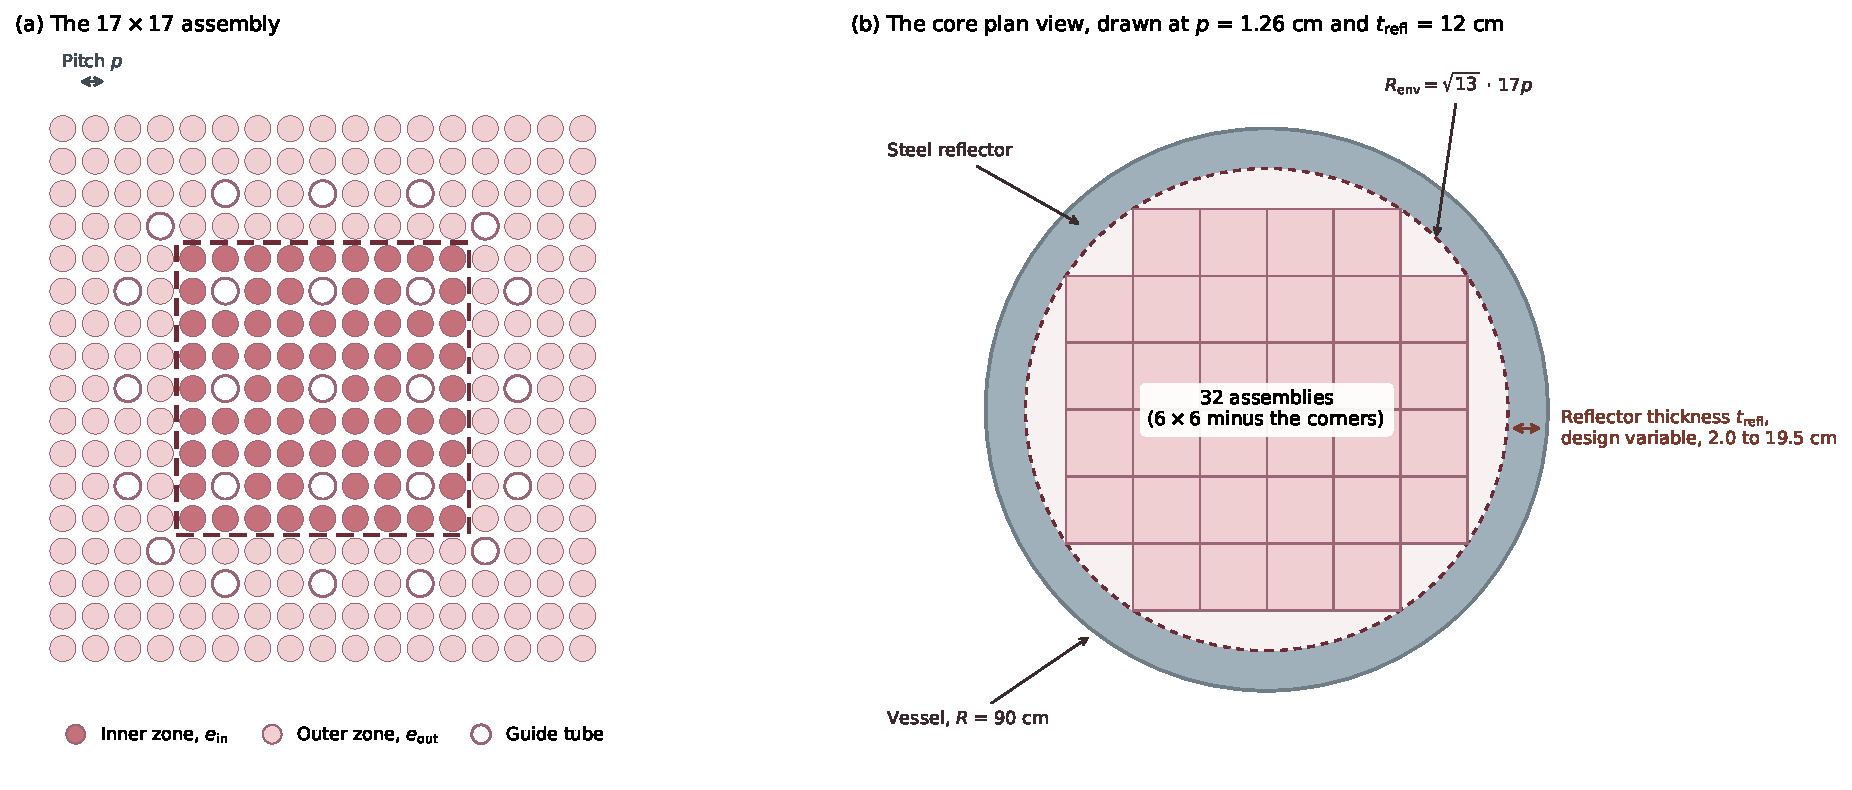
\includegraphics[width=\linewidth]{images/th_model_geometry.pdf}
  \caption{Reference model: assembly and core. (a)~The $17\times17$ assembly. (b)~The core plan view.}
  \label{fig:model-geometry}
\end{figure}

\begin{table}[htbp]
  \centering
  \caption{Geometry of the reference model.}
  \label{tab:model-geometry}
  \begin{tabular}{llc}
    \toprule
    Item & Value & Unit \\
    \midrule
    Fuel pellet outer radius & 0.406 & cm \\
    Cladding inner / outer radius & 0.414 / 0.475 & cm \\
    Guide-tube inner / outer radius & 0.572 / 0.612 & cm \\
    Lattice & $17\times17$: 264 rods, 24 GT, 1 IT & -- \\
    Inner enrichment zone & centred $9\times9$: 72 fuel rods (27\%) & -- \\
    Outer enrichment zone & 192 fuel rods (73\%) & -- \\
    Gd$_2$O$_3$ rods & 12 (C1--C4), discrete 12--40 (C5 on) & -- \\
    Active fuel height & 120 (heavy-metal mass only) & cm \\
    Core map & $6\times6$ minus corners = 32 assemblies & -- \\
    Reflector & stainless steel annulus, thickness $t_\mathrm{refl}$ & -- \\
    Vessel internal radius & 90 & cm \\
    \bottomrule
  \end{tabular}
\end{table}

The vessel internal radius is the 900\,mm inner radius of the simplified
vessel model dimensioned according to CTMSP~\cite{maruyama_2013}, as
detailed in Figure~\ref{fig:vessel-dimensioned}. The pin
and guide-tube dimensions are those of NuScale-class
practice~\cite{nuscale_htp2_2017}. The core thermal power is the
48\,MW of thermal power that the Navy gives for the LABGENE
reactor~\cite{demartini_nuclep_2022}, within the 48 to 50\,MWth of the
academic literature~\cite{dinizcosta_2017}. The active height, the
enrichment zoning, the poisoned-pin pattern, the core map, the
reflector, the temperatures, the soluble boron concentration and the
nuclear data are modelling choices of this thesis.

\begin{table}[htbp]
  \centering
  \caption{Operating and material basis of the reference model.}
  \label{tab:model-operating}
  \begin{tabular}{llc}
    \toprule
    Item & Value & Unit \\
    \midrule
    Core thermal power & 48 & MW \\
    Specific power $P_\mathrm{spec}$ & 9.9834 & W/gHM \\
    Fuel / clad / moderator temperature & 900 / 600 / 580 & K \\
    Soluble boron (fixed, Sec.~\ref{sec:meth-boron}) & 1000 & ppm \\
    Nuclear data & ENDF/B-VII.1 + PWR chain & -- \\
    \bottomrule
  \end{tabular}
\end{table}

In three quantities, the campaign model states its own value instead of
the one given by the reference specification. Each value is kept fixed across the campaigns, so
that every design is evaluated on the same basis and the comparison
between designs is unaffected.

\begin{enumerate}
  \item The heavy reflector is homogenised at \SI{90}{\%} steel by
        volume, a deliberately moderator-rich engineering estimate,
        against \SI{95.6}{\%} in the reference specification.

  \item The control rod absorber radius is \SI{0.433}{cm} for both
        absorbers, against \SI{0.423}{cm} for boron carbide and
        \SI{0.427}{cm} for silver-indium-cadmium in the reference specification.
        The clad radii, \num{0.4369} and \SI{0.484}{cm}, and the
        absorber number densities are those of the reference specification.

  \item The coolant density is \SI{0.72}{g/cm^3} at \SI{580}{K},
        against \SI{0.752}{g/cm^3} implied by the reference-specification number
        densities at its stated \SI{600}{K}. The boron mass fraction
        of \SI{1000}{ppm} is the same in both.
\end{enumerate}

\begin{figure}[htbp]
  \centering
  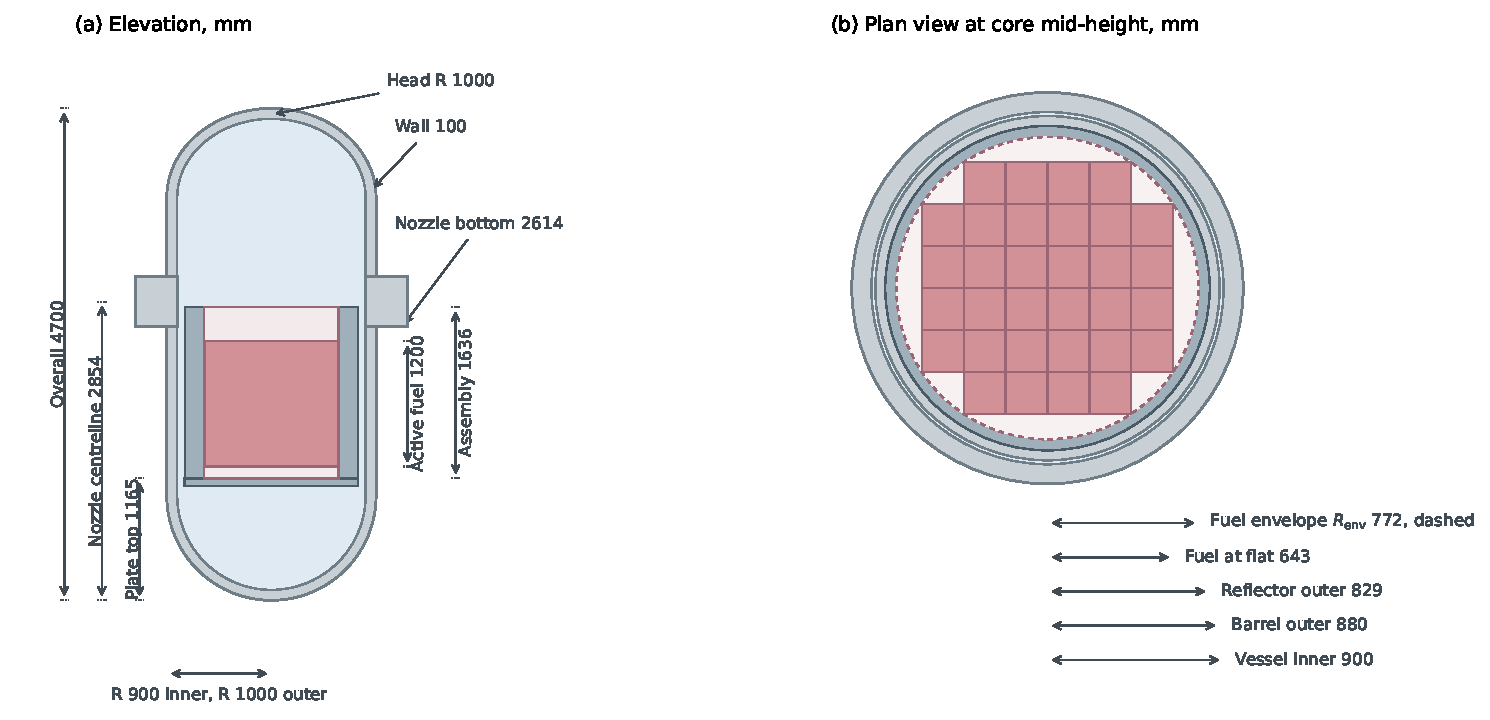
\includegraphics[width=\textwidth]{images/th_vessel_dimensioned}
  \caption{Vessel and core layout: elevation and plan view, in millimetres.}
  \label{fig:vessel-dimensioned}
\end{figure}

The dimensions of Figure~\ref{fig:vessel-dimensioned} come from three
sources, coded as in Table~\ref{tab:in-key}. The vessel envelope, with an overall height of 4700\,mm, a
cylindrical inner radius of 900\,mm, a wall thickness of 100\,mm and a
closure-head inner radius of 1000\,mm, is that of the simplified vessel
model dimensioned according to CTMSP~\cite{maruyama_2013}. The internal
elevations, the lower core plate and the coolant nozzle penetration,
were measured on that same drawing, which carries no dimension for
them, with the overall height as the scale reference, so they carry the
unquantified error of a graphical measurement. The structural components of the fuel assembly,
the nozzles, the end caps, the plenum spring and the spacer grids, keep
the sizes of the NuScale-like reference
specification~\cite{ez_aldeen_2025} without change.

The axial layout combines those two sources. The fixed components are
stacked above the lower core plate at their standard sizes, which
accounts for \SI{435.6}{mm} of the assembly, and the active fuel length
is the remainder up to the coolant nozzle penetration. That remainder is
\SI{1200}{mm}, against the \SI{2000}{mm} of the reference specification,
so the active length is set by the LABGENE-class envelope and not
inherited. The layout is therefore a standard fuel assembly, at
unchanged component sizes, fitted to the space this vessel leaves.

The active height of 120\,cm and the stainless steel reflector annulus
are modelling choices of this thesis, since no open source specifies the
reflector or the core barrel of LABGENE. The plan view of
Figure~\ref{fig:vessel-dimensioned} is constructed for a pin pitch of
1.26\,cm and a reflector thickness of 5.66\,cm, the upper bound of the
design space of Campaigns 8 and 9, at which the downcomer has its
minimum width of 2.0\,cm.

\begin{figure}[htbp]
  \centering
  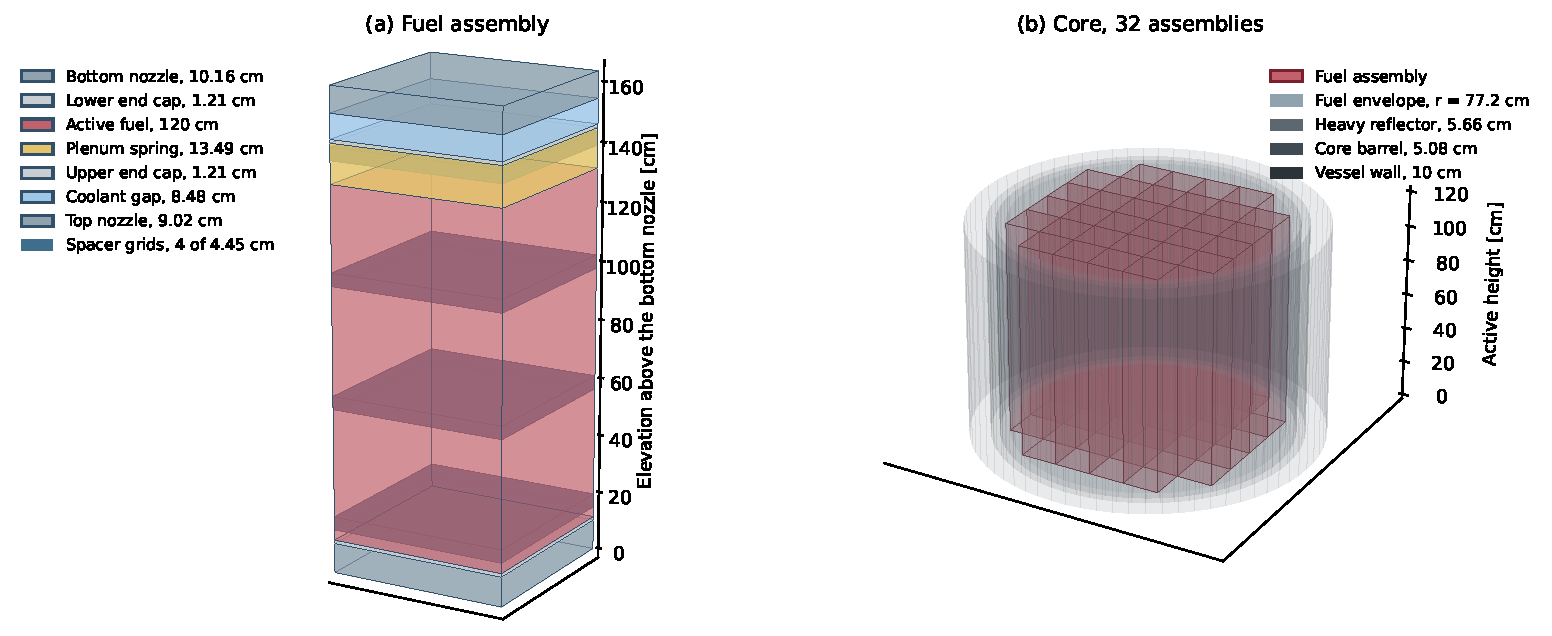
\includegraphics[width=\linewidth]{images/th_model_3d.pdf}
  \caption{Three-dimensional core model: fuel assembly and core.}
  \label{fig:model-3d}
\end{figure}

Figure~\ref{fig:model-3d} shows the assembly and the core in three
dimensions, and Table~\ref{tab:axial-layout} of
Appendix~\ref{app:model-inputs} gives the axial layout adopted for the
three-dimensional core model, with elevations measured from the outer
bottom of the lower head and the assembly resting on the lower core
plate.

The spacer grids take their materials and their height from the
reference specification, one of Inconel followed by three of Zircaloy.
Their number and their spacing are not taken from it. The NuScale-like
reference specification carries five grids at a span of \SI{510.5}{mm} over \SI{2000}{mm} of
active fuel, whereas the shorter active length adopted here carries
four at an equal span of \SI{414}{mm}, of which three are inside the
active fuel and the fourth inside the plenum. The assembly is
\SI{1635.6}{mm} long.

\subsection{Treatment of the barrel and the downcomer in the campaign model}
\label{sec:meth-barrel}

The campaign transport model terminates in a vacuum boundary at the
outer surface of the heavy reflector, so the core barrel, the downcomer
water and the vessel wall of Figure~\ref{fig:vessel-dimensioned} carry
no transport solution. The radial space they occupy is still reserved
in the geometry, from Campaign 8 onward, by the vessel-fit constraint
of Equation~\eqref{eq:ggeom}, which holds the envelope of the core and
its reflector inside the \SI{90}{cm} vessel inner radius. No design is
therefore accepted that would leave those structures with insufficient
radial clearance.

What the omission removes is the albedo of the region behind the
reflector, the fraction of the neutrons leaking from the reflector that
scatter back into the core. That albedo is set by materials and
thicknesses that are the same in every design, and it responds only
weakly to the design variables, so it raises every multiplication factor by nearly
the same amount, shifts every cycle length together and leaves the
ordering of the front unchanged.

\section{Soluble boron treatment}
\label{sec:meth-boron}

The coolant carries a constant concentration of \SI{1000}{ppm} of
natural boron in every campaign of this work. The value is taken from
the operating conditions of the NuScale-like neutronics reference specification
defined by Fridman, Bilodid and
Valtavirta~\cite{fridman_nuscale_benchmark_2023}, together with the
uniform fuel temperature of \SI{900}{\kelvin} adopted in
Table~\ref{tab:model-operating}. The cladding and the steel structures
of that table are at \SI{600}{\kelvin}, and the coolant, which is also
the moderator, at \SI{580}{\kelvin}.

The concentration is a fixed modelling parameter, and no campaign of
this work exposes it to the optimiser as a design variable. Campaign 9 does carry a boron
quantity in its formulation, the critical concentration at the
operating maximum. That quantity is an objective, computed from each
evaluated design and minimised (Section~\ref{sec:meth-c9}), while the
depletion of that campaign is still executed at the fixed \SI{1000}{ppm}.

The specification is static, at Beginning of Life (BOL), and does not
specify a depletion history. The extension of those
conditions to a depleted core is an assumption of the present work and
is discussed as such in Section~\ref{sec:meth-boron-limits}.

\subsection{Basis for the choice}
\label{sec:meth-boron-basis}

Soluble boron is one of the reactivity-control methods of the boron-controlled
PWR lineage from which the present core
inherits its assembly geometry, and it is retained by the majority of
land-based light-water Small Modular Reactor (SMR) concepts now under
development. This work retains it for four reasons:

\begin{enumerate}
  \item \textbf{Traceability of the reference conditions:} the
        NuScale-like reference specification provides a published
        input set, a
        Monte Carlo reference solution obtained with
        Serpent~\cite{fridman_nuscale_benchmark_2023}, and an
        independent reproduction with the same transport code and
        nuclear data library used in this work, namely OpenMC with
        ENDF/B-VII.1~\cite{ez_aldeen_2025}. That
        reproduction reports agreement within 16 to \SI{31}{pcm} in the
        effective multiplication factor and a root mean square relative
        difference below \SI{0.11}{\percent} in assembly radial power.
        No soluble boron specification for the LABGENE-class core that
        motivates the study is available in the open literature.
  \item \textbf{Containment of the design space:} soluble boron and the
        two absorber-related design variables, the gadolinium oxide
        (\ce{Gd2O3}) weight fraction and the gadolinium-bearing pin
        count, act on the same physical quantity, the excess
        reactivity available at the beginning of life. Allowing boron to
        vary would make the study partly a study of boron rather than
        of the fuel and lattice variables under investigation.
  \item \textbf{Scope of the safety demonstration:} a
        Soluble-Boron-Free (SBF) core transfers the entire
        excess-reactivity budget to the burnable absorbers and the
        control rods, so its reactivity control depends on the control rod bank configuration. Three statements bound what this work
        establishes about that configuration.

        \begin{enumerate}[label=\theenumi.\arabic*, ref=\theenumi.\arabic*]
          \item \textbf{The configuration of LABGENE is not available:} no open source gives the number of control
                rod banks of LABGENE, the assemblies each bank occupies,
                the absorber materials or the drive arrangement. The
                layout of Section~\ref{sec:meth-ctrl} is therefore an
                assumption of this work, taken from commercial PWR
                practice at the $17\times17$ guide-tube pattern.

          \item \textbf{The layout supports a first-order
                controllability check:} the constraint applied from
                Campaign 7 measures whether the reactivity worth that
                the regulating banks remove is large enough to keep the
                core subcritical. It establishes
                the order of magnitude of the control requirement and
                rejects designs whose excess reactivity no credible bank
                could compensate. It is not a shutdown margin.

          \item \textbf{A design configuration would need its own
                study:} fixing the banks would require a layout that
                satisfies the reactivity requirement at every state of the
                cycle and is mechanically achievable within the vessel
                head and the guide-tube pattern, together with a Cold
                Shutdown Margin (CSDM) demonstration under the
                single-failure assumption. That demonstration is not
                among the active constraints of any campaign.
        \end{enumerate}

        An SBF core adopted without that study would claim more than
        the present constraints support, so soluble boron is
        carried in every campaign of this work.
  \item \textbf{Known sign of the bias on the objective:} soluble
        boron absorbs part of the excess reactivity of the core, so a
        design evaluated with \SI{1000}{ppm} in the coolant reaches the
        end-of-cycle criterion of Equation~\eqref{eq:eoc} earlier than
        the same design would without boron. Every cycle length
        reported in this work is therefore a lower bound with respect
        to boron-free operation, and the sign of that bias is known
        without further calculation.
\end{enumerate}

Soluble-boron-free operation recurs in the compact and civil marine
light-water designs of the open literature, and its reported
motivations are reviewed in
Section~\ref{subsec:comparison}~\cite{kusunoki_mrx_2000,alam_partI_2019,alzaben_boronfree_2019,ismr_sbf_2024,rr_smr_atf_2025,song_sanchez_2026}.
Reactivity-control practice in operating naval propulsion reactors is
not documented in publicly available sources, and no claim about it is
made here.

\subsection{Declared limitations}
\label{sec:meth-boron-limits}

\begin{enumerate}
  \item The specification from which the concentration is taken is static
        Beginning of Life (BOL) specification. Its extension to a
        depleted core is an assumption of the present work and is not
        supported by the specification itself.
  \item The concentration is kept constant throughout the depletion,
        which is not coupled to a critical boron search. Campaign 9 does search
        for the critical concentration, at beginning of life only, over
        the measured boron points of Section~\ref{sec:meth-c9}, and the
        concentration at the operating maximum is inferred from the
        gadolinium hump through Equation~\eqref{eq:c9-cmax} rather than
        searched. No search is performed at any later burnup step, so
        the depletion trajectory represents a reactivity-tracking model
        and not an operating history. Neither the boron depletion nor
        the burnout of \isotope[10]{B} is modelled.
  \item The MTC is not evaluated inside the optimisation loop, so no
        design is rejected on it. Its boron limit
        (Section~\ref{sec:meth-mtc}) is evaluated in the post-analyses of
        Campaigns 8 and 9, and the values are reported in
        Sections~\ref{sec:res-c8-mtc} and~\ref{sec:res-c9-ceiling}.
\end{enumerate}

\section{Optimisation problem}
\label{sec:meth-problem}

\subsection{Problem statement}

The core design is formulated as a constrained two-objective
optimisation problem over a design space of 4 to 6 decision variables, depending on the campaign (Tables~\ref{tab:design-space}
and~\ref{tab:c89-spec}). The constraints are summarised in
Table~\ref{tab:constraints}.

The first objective maximises the cycle length.

\begin{equation}
\max_{\mathbf{x}\,\in\,\mathcal{X}} \, \mathrm{EFPD}(\mathbf{x})
\label{eq:obj_efpd}
\end{equation}

The second objective minimises the radial peaking factor.

\begin{equation}
\min_{\mathbf{x}\,\in\,\mathcal{X}} \, F_{\Delta H}(\mathbf{x})
\label{eq:obj_fdh}
\end{equation}

This pair of objectives is the one of Campaigns 1 to 8. Campaign 9 keeps
the peaking objective and the evaluator of Campaign 8, and changes the
other half of the problem:

\begin{itemize}
  \item The cycle length leaves the objectives and becomes a constraint
        at the required 5 years.

  \item The critical boron concentration at the most reactive state of
        the cycle becomes the second objective, so both objectives are
        minimised.
\end{itemize}

Equation~\eqref{eq:c9-problem} in Section~\ref{sec:meth-c9} states that
formulation. From Campaign 8 the pitch is fixed at \SI{1.26}{cm} and the
design vector has 4 components against the 6 of the earlier campaigns
(Section~\ref{sec:meth-c8-space}).

Both are subject to the feasibility condition below.

\begin{equation}
g_j(\mathbf{x}) \le 0,
\qquad j = 1,\dots,n_g
\label{eq:constraint_form}
\end{equation}

\noindent where the symbols have the following meaning.

\begin{itemize}
  \item $\mathbf{x}$ is the design vector, whose components and their
        units are listed in Tables~\ref{tab:design-space}
        and~\ref{tab:c89-spec}. It has 5 components in Campaigns 1 to 4, 6 in Campaigns 5 to 7, and 4 in Campaigns 8 and 9.

  \item $\mathcal{X}$ is the box-constrained design space defined by those
        same bounds.

  \item $\mathrm{EFPD}(\mathbf{x})$ is the cycle length of design
        $\mathbf{x}$ in effective full-power days, obtained from
        Equation~\eqref{eq:efpd} with the end-of-cycle criterion of
        Section~\ref{sec:objective_functions}.

  \item $F_{\Delta H}(\mathbf{x})$ is the radial peaking factor of
        design $\mathbf{x}$, dimensionless, defined in
        Equation~\eqref{eq:fdh_definition}.

  \item $g_j(\mathbf{x})$ is the $j$-th inequality constraint of
        Table~\ref{tab:constraints}, expressed in its own native unit
        and feasible when non-positive. The normalisation applied
        before the constraints are aggregated to rank infeasible
        populations is introduced in Campaign 6 and defined in
        Equation~\eqref{eq:cv-norm}.

  \item $n_g$ is the number of active inequality constraints,
        dimensionless: 4 in Campaign 1, 5 in Campaigns 2 to 6, 6 in Campaigns 7 and 8 and 8 in Campaign 9
        (Table~\ref{tab:constraints}). The two-bank reading
        $g_\mathrm{ctrl,12}$ and the boron reading $g_\mathrm{boron}$ of
        Campaign 9 are computed and stored, not constrained.
\end{itemize}

The transport model on which $F_{\Delta H}$ is evaluated changes between
campaigns and is
fixed in Section~\ref{sec:objective_functions}, with the validation
that motivated the change in Section~\ref{sec:meth-core-objective}.

Table~\ref{tab:design-space} gives the design variables and their bounds in Campaigns 1 to 7.

\begin{itemize}
  \item $e_\mathrm{in}$ and $e_\mathrm{out}$, the enrichments of the
        inner and outer zones of the assembly.

  \item $w_\mathrm{Gd}$, the Gd$_2$O$_3$ weight fraction in the
        poisoned rods.

  \item $p$, the pin pitch.

  \item $t_\mathrm{refl}$, the reflector thickness.

  \item $n_\mathrm{Gd}$, the number of gadolinia rods, added as a sixth
        variable in Campaign 5.
\end{itemize}

The design space of Campaigns 8 and 9 is given in
Table~\ref{tab:c89-spec}.

\begin{table}[htbp]
  \centering
  \small
  \caption{Design variables and bounds, Campaigns 1 to 7.}
  \label{tab:design-space}\label{tab:design-space-c56}\label{tab:design-space-c78}
  \begin{tabular}{@{}llccccc@{}}
    \toprule
    Variable & Unit & C1 & C2--C4 & C5 & C6 & C7 \\
    \midrule
    $e_\mathrm{in}$, $e_\mathrm{out}$ & wt\% $^{235}$U & 2.0--19.75 & 2.0--19.75 & 2.0--19.75 & 2.0--17.174 & 3.0--10.43 \\
    $w_\mathrm{Gd}$ & wt\% & 0--8.0 & 0--8.0 & 0--8.0 & 0--8.0 & 0--8.0 \\
    $p$ & cm & 1.15--1.45 & 1.15--1.43 & 1.15--1.43 & 1.15--1.43 & 1.15--1.43 \\
    $t_\mathrm{refl}$ & cm & 2.0--25.0 & 2.0--19.5 & 2.0--19.5 & 2.0--19.5 & 2.0--19.5 \\
    $n_\mathrm{Gd}$ & rods & 12, fixed & 12, fixed & 12--40 & 12--40 & 12--40 \\
    \bottomrule
  \end{tabular}
\end{table}

Figure~\ref{fig:gd-ladder} illustrates the six nested patterns of
gadolinia-bearing pins of Table~\ref{tab:design-space}, each panel showing the pins inherited
from the next lower rod count and the pins added at that count.

\begin{figure}[htbp]
  \centering
  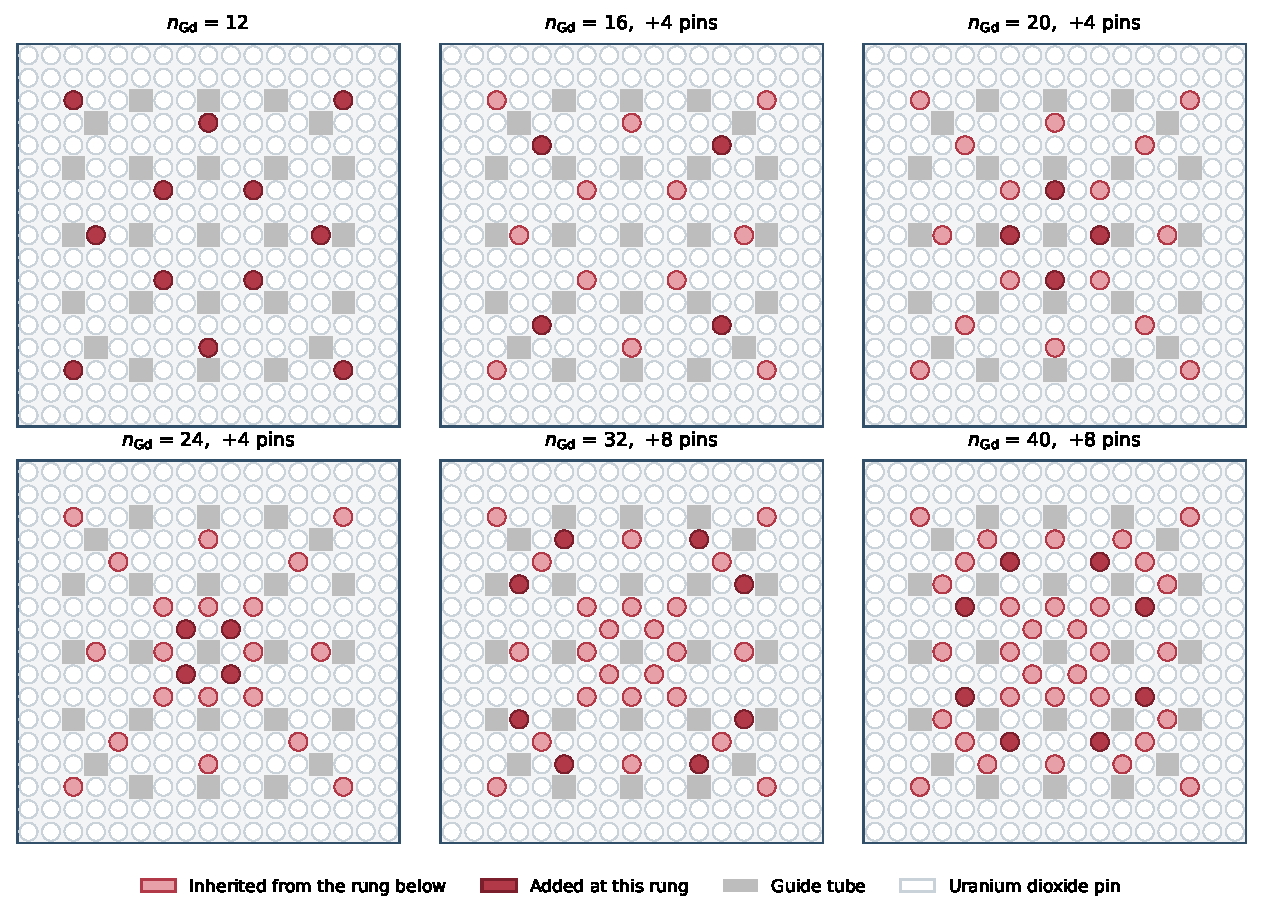
\includegraphics[width=0.92\linewidth]{images/th_gd_ladder.pdf}
  \caption{Gadolinia-bearing pins: the six nested patterns.}
  \label{fig:gd-ladder}
\end{figure}

The gadolinia rod count is a discrete variable, and it reaches the
model in 3 steps:

\begin{enumerate}
  \item NSGA-II represents the rod count as a continuous variable inside
        the bounds, so it proposes values such as 13.845.

  \item The evaluator rounds that value to the nearest admissible
        rod count, one of 12, 16, 20, 24, 32 and 40, before the model
        is built, and an exact midpoint is assigned to the lower count.

  \item The evaluator stores both numbers, the value the optimiser
        proposed and the value that was built.
\end{enumerate}

The positions the added rods take are not free. A gadolinia rod
depresses the thermal flux around itself, so where the rods are placed
changes the assembly peaking factor and the burnout rate of the
absorber at the same rod count. The placement strategy therefore puts
each new rod in the interior of the assembly, around the guide tubes,
following
the optimised 16, 20 and 24 pin maps of Bae, Mertyurek and
Asgari~\cite{bae_gd_2023} and the arrangements of the reference
specification~\cite{nuscale_htp2_2017,epr_fsar_ch4}, under 4 rules.

\begin{enumerate}
  \item The patterns are nested, so each contains the one below it and
        the twelve-rod heritage arrangement of Campaigns 1 to 4 is the
        smallest of them.
  \item Every pattern is octant-symmetric.
  \item The outer 2 rod rows are kept absorber-free.
  \item Every gadolinia rod is face-adjacent or diagonally adjacent to
        a guide tube, and no 2 gadolinia rods are face-adjacent to
        each other, which limits mutual shadowing.
\end{enumerate}

\begin{table}[htbp]
  \centering
  \small
  \caption{Campaigns 1 to 9: constraints and their evaluation.}
  \label{tab:constraints}
\begin{tabularx}{\textwidth}{
    >{\raggedright\arraybackslash}p{0.15\textwidth}
    >{\raggedright\arraybackslash}p{0.40\textwidth}
    >{\raggedright\arraybackslash}X
}
    \toprule
    Constraint & Definition & Evaluated on \\
    \midrule
    $g_{k\min}$ 
        & $1.02 - k_\mathrm{BOL} \le 0$
        & assembly to C5, \textbf{core} from C6 \\

    $g_{k\max}$ 
        & $k_\mathrm{BOL} - k_{\max} \le 0$
        & assembly to C5, \textbf{core} from C6, 
          $k_{\max}$ of Table~\ref{tab:ctrl-bounds} \\

    $g_\mathrm{enr}$ 
        & $e_\mathrm{zoned,max} - e_\mathrm{lim} \le 0$
        & algebraic, $e_\mathrm{lim}$ per campaign \\

    $g_\mathrm{peak}$ 
        & $F_{\Delta H} - 2.0 \le 0$, 1.65 in C9
        & assembly in C1 to C3, \textbf{core} from C4 \\

    $g_\mathrm{geom}$ 
        & $R_\mathrm{env}(p) + \delta + t_\mathrm{refl} + c_\mathrm{v} - 90 \le 0$
        & core, analytic, radial tolerance $\delta$ of
          Equation~\eqref{eq:ggeom}, clearance $c_\mathrm{v}$ of 
          Section~\ref{sec:meth-c8-space} \\

    $g_\mathrm{ctrl}$ 
        & $k_\mathrm{RE} - 0.99 \le 0$
        & \textbf{core}, the sixteen regulating-bank assemblies in,
          from C7 \\

    $g_\mathrm{ctrl,peak}$
        & $k_\mathrm{RE,peak} - 0.99 \le 0$
        & \textbf{core}, as $g_\mathrm{ctrl}$ at the operating maximum of
          the cycle, C9 \\

    $g_\mathrm{efpd}$
        & $1826 - \mathrm{EFPD} \le 0$
        & assembly depletion, C9 \\

    $g_\mathrm{ctrl,12}$ 
        & $k_\mathrm{RE12} - 0.99$
        & core, first two banks in, from C8, 
          \emph{computed and stored, not constrained} \\

    $g_\mathrm{boron}$
        & $c_\mathrm{max} - c_\mathrm{MTC}$
        & core, C9, $c_\mathrm{MTC} = \SI{2763}{ppm}$,
          \emph{computed and stored, not constrained} \\
    \bottomrule
\end{tabularx}
\end{table}

The bound of $g_\mathrm{peak}$ takes 2 values. Campaigns 1 to 8 use
2.0, a deliberately generous adopted value that keeps the exploratory
search free~\cite{epr_fsar_ch4}, and Campaign 9 uses 1.65, the
Technical Specification limit of a licensed pressurised water
reactor~\cite{robinson_gd10}, for the reason given in
Section~\ref{sec:meth-c9}. Satisfying either value is a necessary
condition on a candidate design and not a demonstration of compliance.

\subsection{Geometric feasibility}
\label{sec:meth-geom}

The vessel-fit constraint $g_\mathrm{geom}$ uses the circumscribed
envelope of the intact core footprint.

\begin{equation}
R_\mathrm{env}(p) = \sqrt{13}\,\cdot\,17\,p
\label{eq:renv}
\end{equation}

\noindent where the symbols have the following meaning.

\begin{itemize}
  \item $R_\mathrm{env}$ is the circumscribed radius of the fuel
        region, in cm.

  \item $p$ is the pin pitch, in cm.

  \item $17$ is the number of pin cells per assembly side,
        dimensionless, so that $17p$ is the assembly pitch in cm.

  \item $\sqrt{13} \approx 3.606$ is the dimensionless distance from
        the core centre to the outermost fuel corner of the
        $6\times6$-minus-corners map, in assembly pitches. The extreme
        corner is 3 assembly pitches along one axis and 2 along
        the other, so its distance is $\sqrt{3^2 + 2^2} = \sqrt{13}$.
\end{itemize}

The sensitivity of the envelope to the pitch is obtained directly.

\begin{equation}
\frac{\mathrm{d}R_\mathrm{env}}{\mathrm{d}p} = 61.3~\mathrm{cm\,cm^{-1}}
\label{eq:drenv}
\end{equation}

A pitch increase of one millimetre therefore consumes about
\SI{6.1}{cm} of radial budget. Pitch and reflector thickness compete
directly for the fixed allowance of the 90\,cm vessel internal radius
of Table~\ref{tab:model-geometry}, which makes the 2 variables
strongly coupled.

The enforced form of the constraint carries two further terms. The
geometry builder adds a radial tolerance at the lattice corner, and
Campaign 8 reserves a clearance for the core barrel and the downcomer.
\begin{equation}
g_\mathrm{geom} \;=\; R_\mathrm{env}(p) \;+\; \delta \;+\;
t_\mathrm{refl} \;+\; c_\mathrm{v} \;-\; R_\mathrm{v} \;\le\; 0
\label{eq:ggeom}
\end{equation}

\noindent where the symbols have the following meaning.

\begin{itemize}
  \item $R_\mathrm{env}(p)$ is the circumscribed radius of
        Equation~\eqref{eq:renv}, in cm.

  \item $\delta$ is the radial tolerance of the geometry builder at the
        lattice corner, \SI{0.02}{cm}, a single constant shared by the
        builder and the constraint.

  \item $t_\mathrm{refl}$ is the reflector thickness, in cm.

  \item $c_\mathrm{v}$ is the reserved barrel and downcomer clearance,
        in cm. It is zero in Campaigns 1 to 7 and \SI{7.08}{cm} in
        Campaigns 8 and 9, as derived in
        Section~\ref{sec:meth-c8-space}.

  \item $R_\mathrm{v}$ is the vessel internal radius, \SI{90}{cm}.
\end{itemize}

The tolerance $\delta$ is part of the constraint because in Campaign 4 the
design at $p = \SI{1.150}{cm}$ and $t_\mathrm{refl} = \SI{19.49}{cm}$
satisfied $g_\mathrm{geom}$ by \SI{0.020}{cm}, while the outer radius of its
reflector, built with $\delta$, reached the \SI{90.00}{cm} vessel radius
and the model could not be built.

The constraint is tested analytically inside the optimiser, before any
geometry is built, so a design that cannot fit the vessel is rejected
without spending a transport evaluation on it.

\subsection{Multiplication factor of the reactivity window}
\label{sec:meth-kbasis}

Campaigns 1 to 5 applied the reactivity window to the infinite
multiplication factor of the assembly, $k_\infty$. From Campaign 6 both
bounds act on the effective multiplication factor of the core at
beginning of life, $k_\mathrm{eff}^\mathrm{core}$, which the core solve of the
peaking objective already computes.

\begin{equation}
1.02 \;\le\; k_\mathrm{eff}^\mathrm{core}(\mathbf{x}) \;\le\; k_{\max}
\label{eq:k-window-core}
\end{equation}

\noindent where the symbols have the following meaning.

\begin{itemize}
  \item $k_\mathrm{eff}^\mathrm{core}$ is the effective multiplication
        factor of the 32-assembly core at the beginning of life,
        dimensionless, from the same core solve on which the peaking
        objective is tallied.

  \item $\mathbf{x}$ is the design vector of
        Table~\ref{tab:design-space}.

  \item $k_{\max}$ is the upper reactivity bound of the campaign,
        dimensionless, an adopted 1.35 in Campaigns 1 to 6 and derived
        from the measured bank worth in Campaigns 7 to 9, 1.126 in
        Campaign 7 and 1.166 in Campaigns 8 and 9
        (Table~\ref{tab:ctrl-bounds}).
\end{itemize}

The change of basis acts differently on the two bounds:

\begin{itemize}
  \item \textbf{Upper bound:} with 1.35 on $k_\infty$ the designs of
        Campaigns 4 and 5 include no feasible one, while on
        $k_\mathrm{eff}^\mathrm{core}$ 1.35 is the smallest bound at which
        they do (Section~\ref{sec:res-c5-kbasis}).
  \item \textbf{Lower bound:} the reflective assembly has no leakage, so
        1.02 on $k_\infty$ rejects almost no design. The core factor
        $k_\mathrm{eff}^\mathrm{core}$ includes the radial leakage and is
        several thousand pcm lower for the same design, so 1.02 on it
        rejects the designs that cannot reach criticality.
\end{itemize}

\subsection{Controllability constraint and the upper reactivity bound}
\label{sec:meth-ctrl}

In Campaigns 1 to 6 the adopted bound of 1.35 limits the excess
reactivity the search may accumulate while the objective is the cycle
length, and the transport model carries no control rods. The five-bank scheme
of Figure~\ref{fig:cr-banks} and the constraint below were defined in
the post-analysis of the designs evaluated in Campaign 6 and entered the
active constraints in Campaign 7.

The constraint replaces the adopted value with a measurement. Every
evaluation of Campaign 7 solves the beginning-of-life core twice, and
every evaluation of Campaigns 8 and 9 three times, one per rod
configuration:

\begin{enumerate}
  \item With every bank withdrawn, which gives the peaking objective
        and the unrodded effective multiplication factor $k_\mathrm{eff}^\mathrm{core}$.

  \item With the four regulating banks inserted, which gives
        $k_\mathrm{RE}$, the rodded multiplication factor on which the constraint acts.

  \item From Campaign 8, with the first two regulating banks inserted,
        which gives $k_\mathrm{RE12}$.
\end{enumerate}

The regulating banks RE1 to RE4 occupy the 16 central assemblies and
carry B$_4$C absorbers, and the shutdown bank occupies the outer 16 and
stays withdrawn throughout. The control rod assembly is that of the NuScale-like reference
specification~\cite{fridman_nuscale_benchmark_2023}, with the absorber
materials, boron carbide and silver-indium-cadmium, their number
densities, the cladding, the end plug and the guide tube taken from it
and the absorber radius as the one exception listed in
Section~\ref{sec:reactor-model}. Only the axial dimensions differ,
because the active height of this core is \SI{120}{cm} against
\SI{200}{cm} in the reference specification:

\begin{itemize}
  \item \textbf{Two-dimensional evaluator:} every guide tube of a rodded
        assembly contains B$_4$C over the whole fuel height.

  \item \textbf{Three-dimensional core model:} the rod keeps the axial
        stack of the reference specification with the B$_4$C section
        shortened to the active height, so the bottom \SI{12.04}{cm} of
        the fuel is unrodded, \SI{30.48}{cm} of Ag-In-Cd are above it and
        B$_4$C covers the remaining \SI{77.48}{cm}.
\end{itemize}

\begin{figure}[htbp]
  \centering
  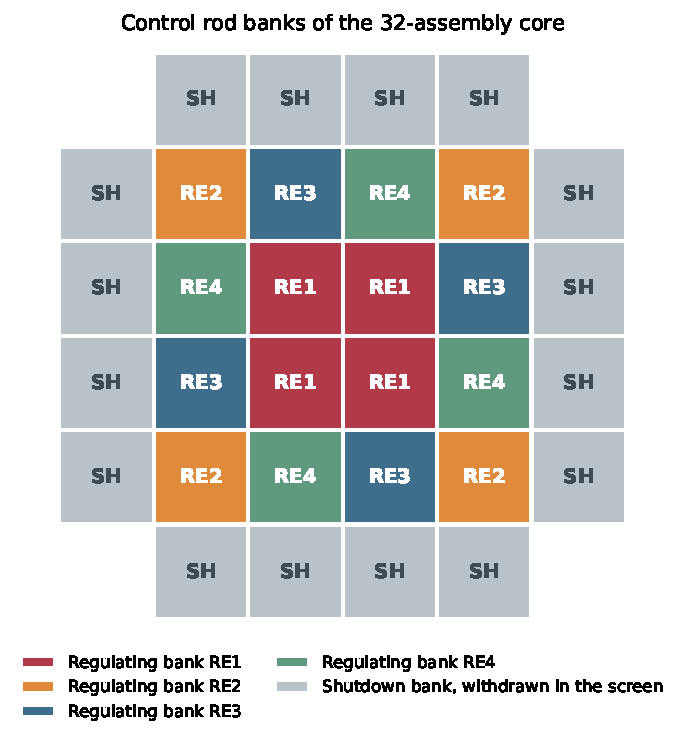
\includegraphics[width=0.52\linewidth]{images/th_cr_banks.pdf}
  \caption{32-assembly core: control rod banks.}
  \label{fig:cr-banks}
\end{figure}

\begin{equation}
k_\mathrm{RE}(\mathbf{x}) = k_\mathrm{eff}^\mathrm{core}\big(\mathbf{x},\ \mathrm{RE1\ to\ RE4\ inserted}\big)
\label{eq:k-re}
\end{equation}

\noindent where the symbols have the following meaning.

\begin{itemize}
  \item $k_\mathrm{RE}$ is the core effective multiplication factor at
        beginning of life with the four regulating banks inserted,
        16 control rod assemblies, and the shutdown bank
        withdrawn, dimensionless.

  \item $\mathbf{x}$ is the design vector.
\end{itemize}

The constraint requires an operating subcriticality margin.

\begin{equation}
g_\mathrm{ctrl}(\mathbf{x}) = k_\mathrm{RE}(\mathbf{x}) - (1 - \Delta\rho_\mathrm{op}) \le 0
\label{eq:g-ctrl-meth}
\end{equation}

\noindent where the symbols have the following meaning.

\begin{itemize}
  \item $g_\mathrm{ctrl}$ is the constraint value, dimensionless,
        negative when satisfied.

  \item $\Delta\rho_\mathrm{op}$ is the operating margin, \num{0.01} in
        units of $k$, that is \SI{1000}{pcm}.
\end{itemize}

The worth of the regulating banks is read from the same pair of solves,
as the difference of the reactivities of the unrodded and the rodded
core.

\begin{equation}
\rho_\mathrm{bank}(\mathbf{x}) = \frac{1}{k_\mathrm{RE}(\mathbf{x})} - \frac{1}{k_\mathrm{eff}^\mathrm{core}(\mathbf{x})}
\label{eq:bank-worth}
\end{equation}

\noindent where the symbols have the following meaning.

\begin{itemize}
  \item $\rho_\mathrm{bank}$ is the reactivity worth of the four
        regulating banks, dimensionless, reported in pcm after
        multiplication by $10^5$.

  \item $k_\mathrm{eff}^\mathrm{core}$ is the unrodded core effective
        multiplication factor at beginning of life, dimensionless.
\end{itemize}

The margin of \SI{1000}{pcm} is an assumption of this work. Its value
is within the standard range of shutdown-margin requirements, at least
\SI{1000}{pcm} under the KTA safety criteria
\cite{alzaben_boronfree_2019,song_sanchez_2026} and at least
\SI{1.0}{\%}~$\Delta k/k$ for the MRX design \cite{kusunoki_mrx_2000},
but those requirements apply to the cold zero-power state with every
rod inserted except the one of highest worth. Here the margin is applied
at hot conditions with the regulating banks alone, so it is not a
licensing shutdown margin. The constraint
therefore tests whether the regulating system can keep the fresh core subcritical at power conditions.

The configuration of $k_\mathrm{RE12}$ inserts only the 8
assemblies of banks RE1 and RE2, the 4 central assemblies and the
4 diagonal assemblies of the middle ring. It is computed and stored
from Campaign 8 as $g_\mathrm{ctrl,12}$ and not constrained, so that the
post-analysis can divide the front into designs controllable with two
banks and designs that need all four, and the margin $M_{8}$ of
Table~\ref{tab:c8-post-boron} is that of this insertion.

The upper reactivity bound of $g_{k\max}$ can now be derived from the
measured bank worth rather than adopted. A design is controllable by
the regulating banks when its excess reactivity,
$1 - 1/k_\mathrm{eff}^\mathrm{core}$, does not exceed its bank worth
less the operating margin. Assuming for every design the smallest worth
measured on a sample of designs turns that condition into a bound on the unrodded multiplication factor.

\begin{equation}
k_{\max} = \frac{1}{1 - \big(\min_{\mathbf{x} \in \mathcal{S}} \rho_\mathrm{bank}(\mathbf{x}) - \Delta\rho_\mathrm{op}\big)}
\label{eq:k-max-derived}
\end{equation}

\noindent where the symbols have the following meaning.

\begin{itemize}
  \item $k_{\max}$ is the derived bound on the unrodded core effective multiplication factor, dimensionless.

  \item $\rho_\mathrm{bank}$ is the reactivity worth of
        Equation~\eqref{eq:bank-worth}, dimensionless.

  \item $\Delta\rho_\mathrm{op}$ is the operating margin of
        Equation~\eqref{eq:g-ctrl-meth}, \num{0.01}.

  \item $\mathcal{S}$ is the sample of designs on which the worth was
        measured.
\end{itemize}

Table~\ref{tab:ctrl-bounds} lists the bounds used and derived. Its
three-dimensional value comes from the eight designs of
Table~\ref{tab:c6-kmax} solved on the three-dimensional core model, where
the smallest difference, 0.14307, is that of C6-59.

\begin{table}[htbp]
  \centering
  \caption{Campaigns 1 to 9: upper reactivity bounds and their sources.}
  \label{tab:ctrl-bounds}
  \small
  \begin{tabularx}{\textwidth}{@{}>{\raggedright\arraybackslash}p{0.16\textwidth}c>{\raggedright\arraybackslash}p{0.20\textwidth}>{\raggedright\arraybackslash}X@{}}
    \toprule
    Campaigns & $k_{\max}$ & Basis & Source \\
    \midrule
    C1 to C6 & 1.35  & assembly, then core & adopted value \\
    retrospective & 1.368 & core, 2D & all 32 control rod assemblies, \SI{1000}{pcm}, eight C6 designs \\
    C7 & 1.126 & core, 2D & four regulating banks, eight C6 designs (Table~\ref{tab:c6-kmax}) \\
    C7 measured & 1.113 to 1.285 & core, 2D & implied by each design's own worth, 60 designs \\
    C8 and C9 & 1.166 & core, 2D from 3D & 0.99 plus the smallest 3D difference of multiplication factors, 0.14307, times $L_\mathrm{ax}$ \\
    \bottomrule
  \end{tabularx}
\end{table}

A bound derived this way has two weaknesses. The minimum of a small
sample is a biased estimate of the minimum of the population, and the quantity it approximates is measured on every evaluation from Campaign
7.

The bound of Campaigns 8 and 9 was computed from the difference of the multiplication factors $k_\mathrm{eff}^\mathrm{core} - k_\mathrm{RE}$ in place of
the reactivity worth, which gives 1.166 against the 1.169 of
Equation~\eqref{eq:k-max-derived} on the same three-dimensional solves.
The difference changes the feasibility of no design.

\begin{table}[!htb]
  \centering
  \small
  \caption{Campaign 6, eight designs: beginning-of-life multiplication factors and bank worths.}
  \label{tab:c6-kmax}
  \begin{tabular}{lcccccc}
    \toprule
    & \multicolumn{2}{c}{All rods out} & \multicolumn{2}{c}{Regulating banks} & \multicolumn{2}{c}{All rods in} \\
    \cmidrule(lr){2-3}\cmidrule(lr){4-5}\cmidrule(lr){6-7}
    Design & $k_\mathrm{eff}^\mathrm{core}$ & Excess & $k_\mathrm{RE}$ & Worth & $k_\mathrm{eff}$ & Worth \\
    & [--] & [pcm] & [--] & [pcm] & [--] & [pcm] \\
    \midrule
    C6-59  & 1.07098 & \num{6627}  & 0.92319 & \num{14947} & 0.69209 & \num{51118} \\
    C6-110 & 1.13466 & \num{11868} & 0.99559 & \num{12310} & 0.80588 & \num{35956} \\
    C6-107 & 1.17396 & \num{14818} & 1.01485 & \num{13355} & 0.78569 & \num{42094} \\
    C6-26  & 1.19152 & \num{16073} & 1.03985 & \num{12242} & 0.89195 & \num{28187} \\
    C6-7   & 1.24287 & \num{19541} & 1.07953 & \num{12174} & 0.92303 & \num{27880} \\
    C6-101 & 1.24592 & \num{19738} & 1.07673 & \num{12612} & 0.91503 & \num{29024} \\
    C6-85  & 1.26157 & \num{20733} & 1.08714 & \num{12718} & 0.86297 & \num{36613} \\
    C6-86  & 1.27869 & \num{21795} & 1.10044 & \num{12668} & 0.92980 & \num{29346} \\
    \bottomrule
  \end{tabular}
\end{table}

\label{sec:res-c6-kmax}

The worth of the scheme was measured in the post-analysis of
Campaign 6 on 8 designs of that campaign, whose excess reactivity
ranges from \num{6627} to \SI{21795}{pcm}, each solved at beginning of
life with all rods out, with the four regulating banks inserted and with
all 32 control rod assemblies inserted (Table~\ref{tab:c6-kmax}). The
all-rods-in configuration measures the largest reactivity the control
rods of a design can remove from the core, although a rod in every
assembly has not been verified to be mechanically feasible.

For the regulating banks the smallest worth of Table~\ref{tab:c6-kmax}
is \SI{12174}{pcm}, on C6-7, and with the operating margin it gives
$1/[1 - (0.12174 - 0.01)] = 1.126$, the bound of Campaign 7.

Figure~\ref{fig:c6-kmax} shows the construction, in which the curve of
the smallest worth intersects the limit of 0.99 at the bound. Because
the bound assumes the smallest worth for every design, it rejects a
design whose own, larger worth would keep it below 0.99, a false
rejection.

\begin{figure}[htbp]
  \centering
  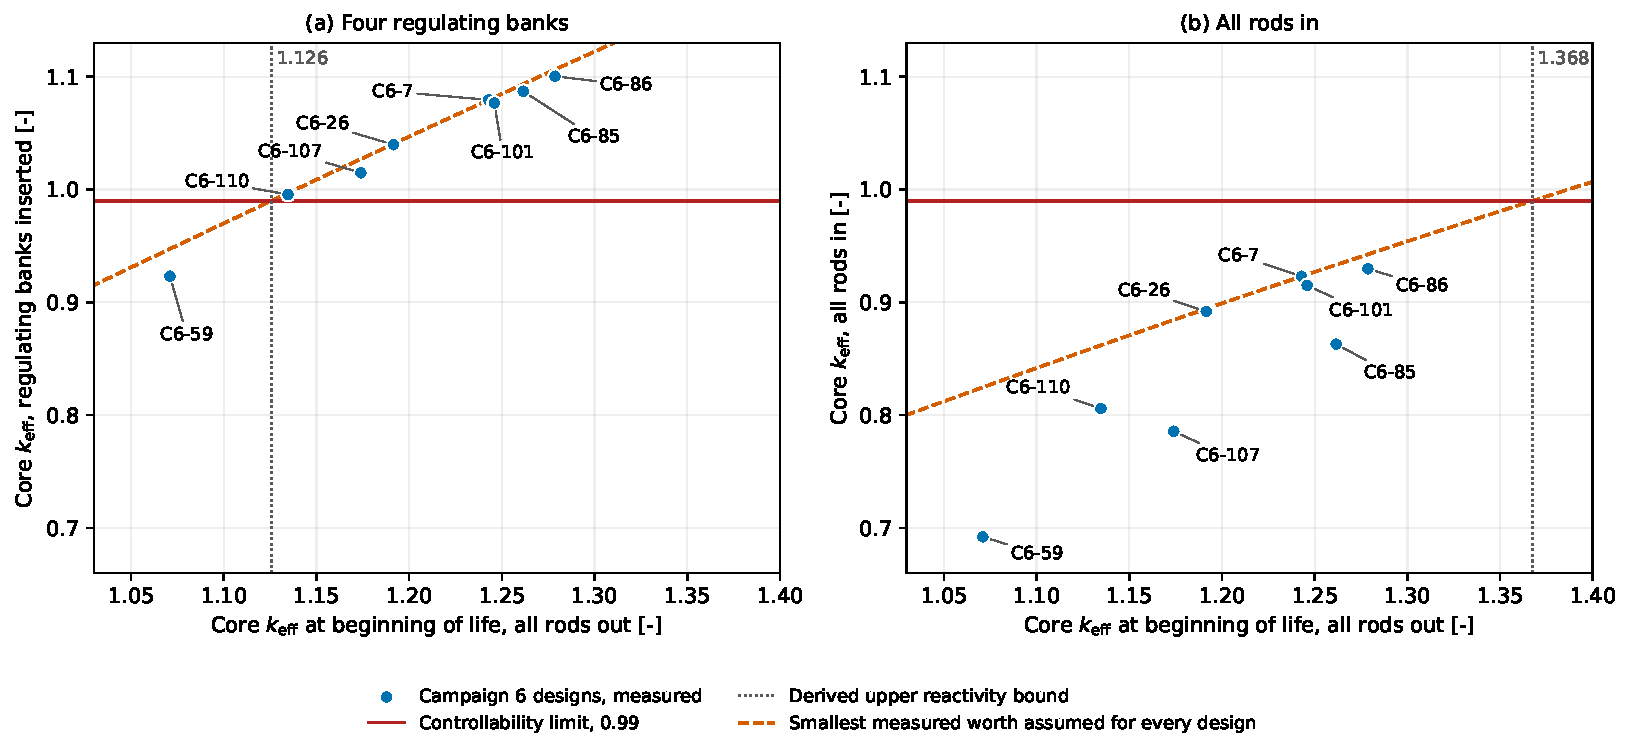
\includegraphics[width=\linewidth]{images/c6_derived_bound}
  \caption{Campaign 6, eight designs: rodded against unrodded core multiplication factor and upper reactivity bound.}
  \label{fig:c6-kmax}
\end{figure}

\label{sec:res-c7-screens}
Campaign 7 then added the measured constraint to the loop and executed
60 evaluations (Figure~\ref{fig:c7-front-screen}). Sixteen designs
satisfy every constraint and their Pareto front has 3 members, and 14 satisfy every constraint except the derived bound of 1.126
while their rodded multiplication factor does not exceed 0.99, so they
are false rejections of the bound. Without the bound 3 of them join the front, which then reaches a core $F_{\Delta H}$ of 1.525 against
1.565 with it, so the bound removed the low-peaking end of the front.
From Campaign 8 the measured constraint is therefore the binding
constraint and the derived value a redundant one.

\begin{figure}[htbp]
  \centering
  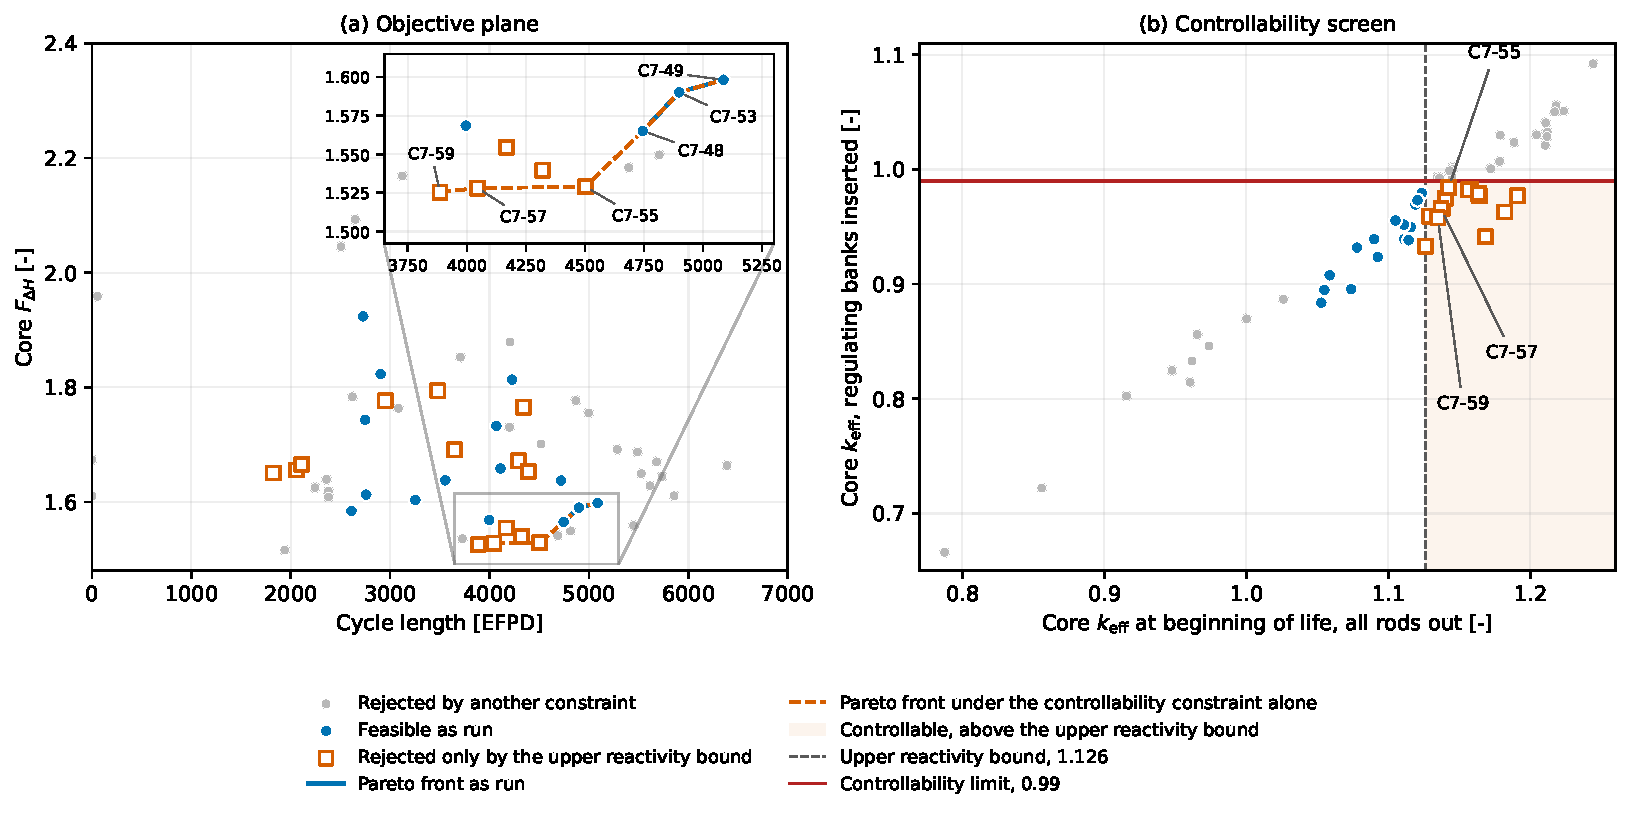
\includegraphics[width=\linewidth]{images/c7_front_screen}
  \caption{Campaign 7: Pareto front and controllability. (a)~Objective plane, with the front as executed and under the controllability constraint alone. (b)~Rodded against unrodded core multiplication factor.}
  \label{fig:c7-front-screen}
\end{figure}

\subsection{Radial zoning and enrichment bounds}
\label{sec:meth-zoning}

From Campaign 6, the beginning-of-life core map is zoned radially inside
the evaluator, so the peaking objective and the peaking constraint act
on the zoned core rather than on a uniform loading.

The 32-assembly map is partitioned into three concentric rings by the
Euclidean distance of each assembly position from the centre of the
map, measured in lattice units.

\begin{enumerate}
  \item Ring C, the centre, 4 assemblies at a distance below 1.0.
  \item Ring M, the middle, 12 assemblies at a distance from 1.0 to
        2.3.
  \item Ring P, the periphery, 16 assemblies at a distance of 2.3 or
        above.
\end{enumerate}

Figure~\ref{fig:zoning-rings} shows the three rings on the core map.

\begin{figure}[htbp]
  \centering
  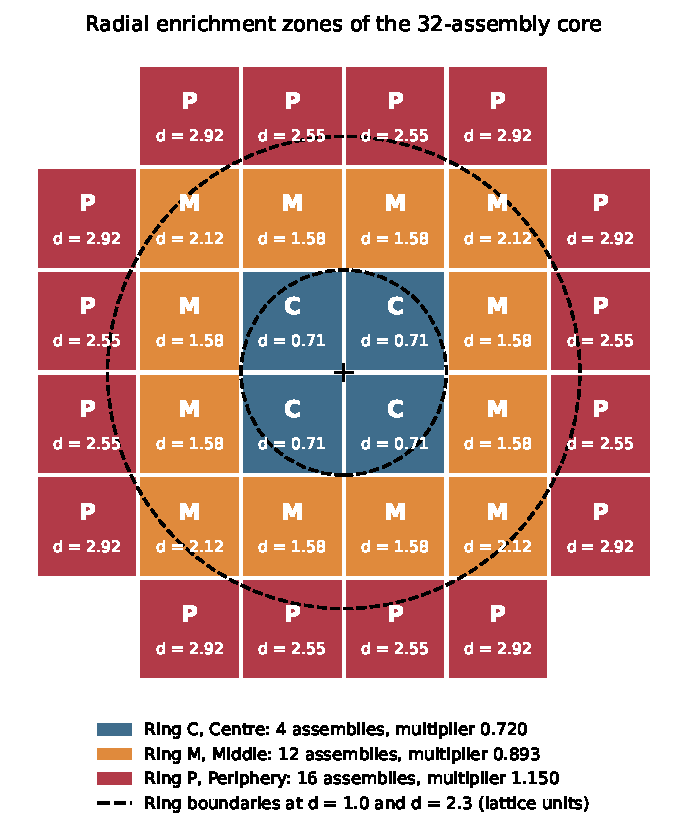
\includegraphics[width=0.5\linewidth]{images/th_zoning_rings.pdf}
  \caption{32-assembly core: radial enrichment rings.}
  \label{fig:zoning-rings}
\end{figure}

The enrichment of each ring is the corresponding design enrichment
scaled by a fixed ring multiplier.

\begin{equation}
e_r \;=\; m_r \, e, \qquad r \in \{C, M, P\}
\label{eq:zoning}
\end{equation}

\noindent where the symbols have the following meaning.

\begin{itemize}
  \item $e_r$ is the as-loaded enrichment of ring $r$, in
        wt\%~$^{235}$U.

  \item $e$ is the design enrichment assigned to that ring, in
        wt\%~$^{235}$U.

  \item $m_r$ is the multiplier of ring $r$, dimensionless, equal to
        $m_C = 0.720$ for the centre, $m_M = 0.893$ for the middle
        ring and $m_P = 1.150$ for the periphery.
\end{itemize}

Only $m_C$ and $m_P$ are set. The middle multiplier is solved from the
fissile balance, which holds the assembly-weighted mean multiplier of
the core at one.

\begin{equation}
n_C\,m_C + n_M\,m_M + n_P\,m_P = n_C + n_M + n_P
\label{eq:zoning-balance}
\end{equation}

\noindent where $n_C$, $n_M$ and $n_P$ are the assembly counts of the
three rings, equal to 4, 12 and 16, dimensionless. With $m_C = 0.720$
and $m_P = 1.150$ the balance returns $m_M = 0.893$, so the zoned core
and an unzoned core built from the same enrichment variables carry the
same fissile inventory.

\subsubsection{How the design enrichments enter the rings}
\label{sec:meth-zoning-map}

The zoning does not assign one design enrichment to one ring. Through
Campaign 7, every assembly of the core keeps the two-zone
intra-assembly structure of Table~\ref{tab:model-geometry}, illustrated in
Figure~\ref{fig:model-geometry}(a), namely the centred $9\times9$ block
of 72 rods at $e_\mathrm{in}$ and the surrounding 192 rods at
$e_\mathrm{out}$. What the ring multiplier does is scale \emph{both}
intra-assembly enrichments of every assembly in that ring by the same
factor. From Campaign 8, the two zones collapse to the single enrichment
variable of Section~\ref{sec:meth-c8-space}, and the multiplier scales
that one value.

\begin{equation}
e_\mathrm{in}^{\,r} = m_r \, e_\mathrm{in},
\qquad
e_\mathrm{out}^{\,r} = m_r \, e_\mathrm{out}
\label{eq:zoning-pair}
\end{equation}

\noindent where the symbols have the following meaning.

\begin{itemize}
  \item $e_\mathrm{in}^{\,r}$ and $e_\mathrm{out}^{\,r}$ are the
        as-loaded inner-zone and outer-zone enrichments of an assembly
        in ring $r$, in wt\%~$^{235}$U.

  \item $e_\mathrm{in}$ and $e_\mathrm{out}$ are the 2 enrichment
        design variables, in wt\%~$^{235}$U.

  \item $m_r$ is the multiplier of ring $r$, dimensionless.
\end{itemize}

Three consequences result, and all three are properties of the
implementation rather than modelling choices imposed a posteriori.

\begin{enumerate}
  \item Zoning is an enrichment redistribution only. Pitch, reflector
        thickness, gadolinia weight fraction and gadolinia rod count
        are copied to every ring unchanged, so the three ring
        assemblies are built by the same builders with the same pin
        layout as the base assembly.

  \item The gadolinia rods of each ring take their \ce{^{235}U}
        enrichment from that ring, reduced by 5 per cent, relative per
        wt\% of \ce{Gd2O3}, with a lower limit of \SI{0.2}{wt\%}
        (Table~\ref{tab:in-materials}), following the practice for
        low-concentration gadolinia fuel~\cite{mildrum_segovia_2001}.
        The reduction lowers the fissile
        content of the urania--gadolinia rods, whose thermal conductivity
        is lower than that of \ce{UO2}~\cite{mildrum_segovia_2001}. At
        \SI{8}{wt\%} of \ce{Gd2O3}, for example, the factor is 0.60, so
        the gadolinia rods of a peripheral ring at \SI{11.5}{wt\%} carry
        \SI{6.9}{wt\%}.

  \item The zoning is applied to core solves only. The beginning-of-life
        core solve of Section~\ref{sec:meth-core-objective} and the 2
        rodded solves of Section~\ref{sec:meth-ctrl} are built from the
        zoned map, while the depletion of
        Section~\ref{sec:objective_functions} is executed on the assembly
        loaded at the design enrichments themselves, with no multiplier
        applied, that is $m = 1$ in
        Equation~\eqref{eq:zoning-pair}. That assembly is none of the
        three rings. It carries the core-average fissile loading, since
        the balance of Equation~\eqref{eq:zoning-balance} holds the
        assembly-weighted mean multiplier at one, and the reflective
        boundary of the depletion model replicates it into an infinite
        lattice of identical assemblies. The burnup history obtained is
        therefore the history of a core of 32 identical assemblies, whose
        fissile inventory equals that of the zoned core.
\end{enumerate}

The gadolinia loading of a design is measured in two ways in the
post-analyses, by the weight fraction $w_\mathrm{Gd}$ and by the
inventory $I_\mathrm{Gd}$, which is proportional to the mass of
gadolinia per assembly.

\begin{equation}
I_\mathrm{Gd} = w_\mathrm{Gd}\, n_\mathrm{Gd}
\label{eq:gd-inventory}
\end{equation}

\noindent where $I_\mathrm{Gd}$ is the gadolinia inventory, in wt\%
times pins, $w_\mathrm{Gd}$ the gadolinia weight fraction, in wt\%, and
$n_\mathrm{Gd}$ the number of poisoned pins.

\subsubsection{The enrichment search range}
\label{sec:meth-zoning-box}

Because the periphery carries the largest multiplier, the LEU
enrichment limit binds through the as-loaded peripheral ring
and not through the design variable directly. From Campaign 6, the
enrichment constraint is therefore written on the zoned map.

\begin{equation}
g_\mathrm{enr} \;=\; \max_r \left( m_r\, e \right) - e_\mathrm{lim} \;\le\; 0
\quad\Longrightarrow\quad
e \;\le\; \frac{e_\mathrm{lim}}{m_P}
\label{eq:leu-box}
\end{equation}

\noindent where the symbols have the following meaning.

\begin{itemize}
  \item $g_\mathrm{enr}$ is the enrichment-limit constraint of
        Table~\ref{tab:constraints}, in wt\%~$^{235}$U, redefined on
        the zoned map from Campaign 6.

  \item $e_\mathrm{lim}$ is the enrichment limit of the campaign, in
        wt\%~$^{235}$U, 19.75 in Campaign 6, 12 in Campaign 7 and 16 in
        Campaigns 8 and 9 (Table~\ref{tab:cv-scales}).

  \item $m_P$ is the peripheral multiplier, dimensionless, equal to
        1.150.

  \item $e_\mathrm{lim}/m_P$ is the resulting upper bound of the
        enrichment design variables, 17.174, 10.43 and 13.913
        wt\%~$^{235}$U in the same campaigns. The limit of 16 of
        Campaigns 8 and 9 places this bound close to the \SI{13.8}{wt\%}
        above which every design of Campaign 6 violated the upper
        reactivity bound (Section~\ref{sec:res-history}), so the
        evaluation budget is not spent on a region that returns
        infeasible designs.
\end{itemize}

The bound and the constraint are consistent by construction, so no
design of experiments point can violate the limit after zoning. This
removes the wasted samples observed under the earlier formulation, and
it is also what gives $m_P$ its upper limit.

The value of $m_P$ is the only decision of this subsection that is not
fixed by a measurement. A larger multiplier lowers the radial peaking
factor further, but it lowers the upper enrichment bound of
Equation~\eqref{eq:leu-box} in the same proportion, and the enrichment
limit was already active in Campaign 5. Campaign 6 therefore adopts
$m_P = 1.150$, keeping the wider enrichment range at the cost of that
peaking reduction, and a later campaign can raise $m_P$ if the
enrichment bound is no longer active.

The zoning is the only change of Campaign 6 that acts on the
beginning-of-life power distribution, so the peaking reduction of
Campaign 6 is attributed to it (Section~\ref{sec:res-c6-compare}).

\subsection{Objective functions}
\label{sec:objective_functions}

\subsubsection{Cycle length}
\label{sec:meth-cycle-length}

The cycle length is an objective in Campaigns 1 to 8 and a constraint in
Campaign 9, where the five-year requirement enters
Equation~\eqref{eq:c9-problem}. It is computed in the same way in both
cases, from the end-of-cycle burnup through the conversion of
Equation~\eqref{eq:efpd}, with the specific power of
Table~\ref{tab:model-operating}. What remains to be fixed here is the
criterion that defines the end of cycle on the model used for the
depletion, the reflective single assembly.

\begin{equation}
B_\mathrm{EOC} = \min\!\left( B_k,\, B_\mathrm{max} \right)
\label{eq:eoc}
\end{equation}

\begin{equation}
B_k = \min\left\{\, B > 0 \,:\, k_\infty(B) \le k_\mathrm{target} \,\right\}
\label{eq:eoc-k}
\end{equation}

\noindent where the symbols have the following meaning.

\begin{itemize}
  \item $B_\mathrm{EOC}$ is the end-of-cycle burnup entering
        Equation~\eqref{eq:efpd}, in MWd/kgHM.

  \item $B_k$ is the reactivity-defined end-of-cycle burnup, in
        MWd/kgHM.

  \item $B_\mathrm{max}$ is the depletion horizon, in MWd/kgHM
        (Section~\ref{sec:meth-atf}). A design that has not reached
        $k_\mathrm{target}$ at $B_\mathrm{max}$ is stored with
        $B_\mathrm{EOC} = B_\mathrm{max}$, a lower bound.

  \item $B$ is the burnup along the depletion history, in MWd/kgHM.

  \item $k_\infty(B)$ is the infinite multiplication factor of the
        reflective assembly at burnup $B$, dimensionless.

  \item $k_\mathrm{target}$ is the leakage-corrected end-of-cycle multiplication factor, dimensionless, defined in
        Section~\ref{sec:meth-ktarget}.
\end{itemize}

The crossing $B_k$ is obtained by linear interpolation between the 2
consecutive depletion steps between which the residual
$k_\infty - k_\mathrm{target}$ changes sign.

The depletion terminates adaptively at the first step below
$k_\mathrm{target}$, so it advances in blocks, each a separate
depletion call that restarts from the results file of the previous one.
\label{sec:restart_defect}%
A restart requires that file to carry the reaction rates, which the
depletion solver of OpenMC~0.15.3 writes only when the
\texttt{write\_rates} option is set, and its default is false.
Campaigns 2 to 5 restarted without the rates:

\begin{itemize}
  \item \textbf{Defect:} the first step of every restarted block advanced
        by radioactive decay alone while the burnup label advanced by the
        full step, so every restarted depletion stored a label ahead of
        the physical burnup by one marching step of
        \SI{4.0}{\mega\watt\day\per\kilo\gram} per restart, and the cycle
        lengths were too long.
  \item \textbf{Identification:} the defect was found in the stored
        histories and confirmed on design C5-7, depleted twice with the
        same seed, as a single block and as 3 blocks of 2 steps, which
        agree within 56 to \SI{132}{pcm} once the labels are corrected
        (Figure~\ref{fig:c5-restart}).
  \item \textbf{Correction:} the histories of Campaigns 3 to 5 were
        corrected without repeating any depletion, by discarding the duplicated first point
        of each restart and subtracting one marching step per restart from
        the label. Those of Campaign 2 were not corrected, so its stored
        cycle lengths remain ahead of the physical burnup.
\end{itemize}

Campaign 1 is unaffected, since its fixed schedule completes in a single
call. From Campaign 6 the evaluator requests the rates at every block and
stops with an error when a restart file carries none.

\subsubsection{Radial peaking factor}
\label{sec:meth-fdh}

The peaking objective of Equation~\eqref{eq:obj_fdh} uses the radial
peaking factor of Equation~\eqref{eq:fdh_definition}, formally defined
in Section~\ref{sec:bg-peaking}. That definition leaves two
methodological choices open, and both are fixed here:

\begin{itemize}
  \item \textbf{Numerical estimator:} the integrals of
        Equation~\eqref{eq:fdh_definition} are replaced by
their Monte Carlo counterparts. A pin-wise fission energy deposition
tally is accumulated over the active fuel region, so each rod
contributes one volume-integrated score.

\begin{equation}
\widehat{F}_{\Delta H}
=
\frac{\displaystyle \max_{i \in \{1,\dots,N\}} \widehat{P}_i}
     {\displaystyle \frac{1}{N} \sum_{j=1}^{N} \widehat{P}_j}
\label{eq:fdh_estimator}
\end{equation}

\noindent where the symbols have the following meaning.

\begin{itemize}
  \item $\widehat{F}_{\Delta H}$ is the Monte Carlo estimate of the
        radial peaking factor, dimensionless.

  \item $\widehat{P}_i$ is the tallied fission energy deposition rate
        of fuel rod $i$ over the full active height, in W.

  \item $N$ is the number of fuel rods in the evaluation domain,
        dimensionless.

  \item $i$ and $j$ are fuel rod indices, dimensionless.
\end{itemize}

Two properties of this estimator govern the selection methodology.

\begin{enumerate}
  \item The estimate carries a statistical uncertainty inherited from
        the finite number of simulated histories. Differences between
        candidate designs smaller than that uncertainty cannot be
        distinguished statistically by a single evaluation.

  \item The estimate is positively biased. The numerator is the
        maximum over the scores of $N$ fuel rods, each carrying its own
        statistical fluctuation, so fluctuation alone raises the sampled
        maximum above the true maximum. The bias decreases as the
        number of simulated histories increases, because the tally
        variance decreases with it.
\end{enumerate}

  \item \textbf{Evaluation domain:} the tally domain of
        Equation~\eqref{eq:fdh_estimator} determines what the objective
        represents. Two levels are used in this work.

\begin{enumerate}
  \item Assembly level, in which $N$ covers the 264 fuel rods of a
        single reflected assembly. This level is inexpensive and was the
        tally domain of the peaking objective in Campaigns 1 to 3.

  \item Core level, in which $N$ covers the fuel rods of the full
        32-assembly core at the beginning of life. This level is the tally
        domain of both the objective and the peaking constraint from
        Campaign 4 onward.
\end{enumerate}
\end{itemize}

Every campaign solve of this work, at assembly and at core level, is
two-dimensional, an axial segment of the lattice with reflective
boundaries above and below. The reflective boundary makes the segment an
axially infinite medium whose flux does not depend on the axial
coordinate~\cite{openmc_docs,duderstadt_hamilton_1976}, so the fission
energy deposition rate of every rod is uniform along the height, the
common factor $H$ cancels between the numerator and the denominator of
Equation~\eqref{eq:fdh_definition}, and the tally of each rod is already
proportional to the height-integrated quantity from which
Equation~\eqref{eq:fdh_estimator} is formed.

The two-dimensional value equals the three-dimensional one only if the
power distribution is separable into a radial factor and an axial shape
common to every rod. A core of finite height is not separable, because
the axial leakage returned by the axial reflector, the flux depression
of each spacer grid and the absorption of a partially inserted bank all
depend on the radial position of the rod, so the height integral of a
rod is no longer a common multiple of its mid-plane rate and the two
estimators differ. The size of that difference on the front designs is
measured in Section~\ref{sec:res-c9-peaking}.

The assembly estimator is in turn a poor predictor of the core value,
which is what moved the tally domain to core level from Campaign 4. The
study that established this is described in
Section~\ref{sec:meth-core-objective} and its measurements are reported
in Section~\ref{sec:res-corevalidation}.

\subsubsection{Normalisation of the constraint violation}
\label{subsubsec:cv-norm}

The constraints of the problem carry five different units:

\begin{itemize}
  \item \textbf{Multiplication factor:} the reactivity window and the
        controllability constraints.
  \item \textbf{Weight percentage:} the enrichment limit.
  \item \textbf{Dimensionless power ratio:} the peaking limit.
  \item \textbf{Centimetre:} the vessel fit.
  \item \textbf{Day:} the minimum cycle length of Campaign 9.
\end{itemize}

When no member of the population is feasible,
NSGA-II ranks the candidates by their total constraint violation, and a
sum of raw violations weights each constraint by its unit. A vessel-fit
violation of \SI{1}{cm} contributes 1.0 to the sum, 10 times the
contribution of a reactivity violation of \SI{10000}{pcm}, which is 0.1
in units of $k$.

From Campaign 6 onward, each constraint is divided by a scale before it
enters the optimiser.

\begin{equation}
  V = \sum_{j=1}^{n_g} \max\!\left(0, \frac{g_j}{s_j}\right)
  \label{eq:cv-norm}
\end{equation}

\noindent where the symbols have the following meaning.

\begin{itemize}
  \item $V$ is the total constraint violation used to rank infeasible
    candidates, dimensionless.
  \item $g_j$ is the raw value of constraint $j$ in its native unit, with
    $g_j \leq 0$ denoting feasibility.
  \item $s_j$ is the normalisation scale of constraint $j$, taken equal to the
    limit of that constraint, in the same unit as $g_j$.
  \item $n_g$ is the number of inequality constraints, dimensionless.
\end{itemize}

Each scale is the limit of its constraint in the campaign concerned,
and Table~\ref{tab:cv-scales} gives the values. The controllability constraints are the exception, since their
limit is 0.99 while the scale is the critical value of 1.0.

\begin{table}[htbp]
  \centering
  \small
  \caption{Normalisation scales $s_j$ of the constraint violation, Campaigns 6 to 9.}
  \label{tab:cv-scales}
  \begin{tabular}{@{}l l r r r r@{}}
    \toprule
    Constraint & Unit of $g_j$ & C6 & C7 & C8 & C9 \\
    \midrule
    $g_{k\min}$            & $\Delta k$ & 1.02  & 1.02  & 1.02  & 1.02  \\
    $g_{k\max}$            & $\Delta k$ & 1.35  & 1.126 & 1.166 & 1.166 \\
    $g_\mathrm{enr}$       & wt\%       & 19.75 & 12    & 16    & 16    \\
    $g_\mathrm{peak}$      & --         & 2.0   & 2.0   & 2.0   & 1.65  \\
    $g_\mathrm{geom}$      & cm         & 90.0  & 90.0  & 82.92 & 82.92 \\
    $g_\mathrm{ctrl}$      & $\Delta k$ & --    & 1.0   & 1.0   & 1.0   \\
    $g_\mathrm{ctrl,peak}$ & $\Delta k$ & --    & --    & --    & 1.0   \\
    $g_\mathrm{efpd}$      & days       & --    & --    & --    & 1826  \\
    \bottomrule
  \end{tabular}
\end{table}

The normalisation preserves the sign of every $g_j$, so the feasible
set is unchanged, and it acts on the constraint matrix only, so the
objectives and the hypervolume history are unchanged. It orders the
infeasible designs only, because NSGA-II ranks every feasible design
above every infeasible one, so the reported Pareto fronts, which contain
feasible designs only, do not depend on it. The scales are stored in the
checkpoint, and the optimisation program does not resume a campaign
whose constraints differ from the stored ones, so every evaluation of a
campaign is ranked with the same scales.

\section{Campaign structure}
\label{sec:meth-campaigns}

Each campaign changes the problem only where the designs of its
predecessor exposed a defect, so that every observed difference is
attributable to those changes, and Table~\ref{tab:campaign-history}
gives the sequence with the defect that motivated each change.

Campaign 6 applies 4 corrections established on the designs evaluated
in Campaigns 4 and 5:

\begin{itemize}
  \item \textbf{Reactivity window:} both bounds act on the core effective
        multiplication factor (Section~\ref{sec:meth-kbasis}).
  \item \textbf{Radial zoning:} three enrichment rings in the core map
        (Section~\ref{sec:meth-zoning}).
  \item \textbf{Depletion horizon:} raised to \SI{100}{MWd/kgHM}
        (Section~\ref{sec:meth-atf}). The previous horizon stopped the
        depletion before some designs reached $k_\mathrm{target}$, so each
        of them was stored with the same right-censored cycle length, a
        lower bound of the value it would have reached, which the
        optimiser could not rank.
  \item \textbf{Constraint violation:} each constraint normalised by its
        limit (Section~\ref{subsubsec:cv-norm}).
\end{itemize}

Each correction acts on a separate output of the evaluator, so its
effect remains attributable, and testing them one campaign at a time
would have required 3 further campaigns of about 60 transport
evaluations each. Inside Campaign 6, each of the first 3 infill blocks
adds one element of the acquisition function (Section~\ref{sec:meth-acq}).
Campaign 9 changes the formulation (Section~\ref{sec:meth-c9}), the lower
enrichment bound and the division of its 60 evaluations
(Table~\ref{tab:c89-spec}).

\section{Design space and formulation of Campaigns 8 and 9}
\label{sec:meth-c8-space}

The Pareto fronts of Campaigns 8 and 9 are the candidate results of
this work. Campaign 8 narrows the design space
with what the earlier campaigns measured, removing from the search the
regions they showed to return infeasible designs, so that the
evaluation budget is spent where feasible designs exist. Campaign 9
changes the formulation of the problem and extends the enrichment range
down to \SI{2.0}{wt\%}.
Table~\ref{tab:c89-spec} compares the two.

\begin{table}[htbp]
  \centering
  \small
  \caption{Campaigns 8 and 9: design space and formulation.}
  \label{tab:c89-spec}
  \begin{tabular}{@{}l l l@{}}
    \toprule
    Item & Campaign 8 & Campaign 9 \\
    \midrule
    Enrichment $e$                 & 3.0 to \SI{13.913}{wt\%} & 2.0 to \SI{13.913}{wt\%} \\
    Gadolinia fraction $w_\mathrm{Gd}$ & 0 to \SI{8.0}{wt\%}  & 0 to \SI{8.0}{wt\%} \\
    Reflector thickness $t_\mathrm{refl}$ & 2.0 to \SI{5.66}{cm} & 2.0 to \SI{5.66}{cm} \\
    Gadolinia rods $n_\mathrm{Gd}$ & discrete, 12 to 40     & discrete, 12 to 40 \\
    Pin pitch                      & fixed, \SI{1.26}{cm}   & fixed, \SI{1.26}{cm} \\
    Clearance $c_\mathrm{v}$       & \SI{7.08}{cm}          & \SI{7.08}{cm} \\
    \midrule
    Objectives                     & max EFPD, min $F_{\Delta H}$ & min $F_{\Delta H}$, min $c_\mathrm{max}$ \\
    Cycle length                   & objective              & constraint, $\ge 1826$ EFPD \\
    Peaking bound                  & 2.0                    & 1.65 \\
    Controllability                & beginning of life      & beginning of life and operating maximum \\
    \midrule
    Evaluations                    & 36 + $4\times6$ = 60   & 24 + $6\times6$ = 60 \\
    \bottomrule
  \end{tabular}
\end{table}

\subsection{Design space}

Four decisions define the design space of Campaign 8, and Campaign 9
changes only the lower enrichment bound:

\begin{enumerate}
  \item The pin pitch is fixed at \SI{1.26}{cm}, the rod pitch of the
        Westinghouse $17\times17$ assembly~\cite{todreas_kazimi_2012}
        and of the NuScale fuel assembly~\cite{nuscale_htp2_2017}, which
        the reference fuel design of Section~\ref{sec:design-basis}
        already adopts. Three findings led to this decision.

        \begin{itemize}
          \item Below \SI{1.224}{cm} the boundary of the lattice cell
                truncates the guide-tube wall without a warning from the
                code. At the lower
                pitch bound of \SI{1.150}{cm} up to \SI{28}{\%} of the
                wall is replaced by moderator
                (Figure~\ref{fig:gt-clip}). Twenty-five of the 60
                Campaign 7 designs, and designs of every earlier
                campaign, are in this range
                (Section~\ref{sec:res-c7-limits}).

\begin{figure}[htbp]
  \centering
  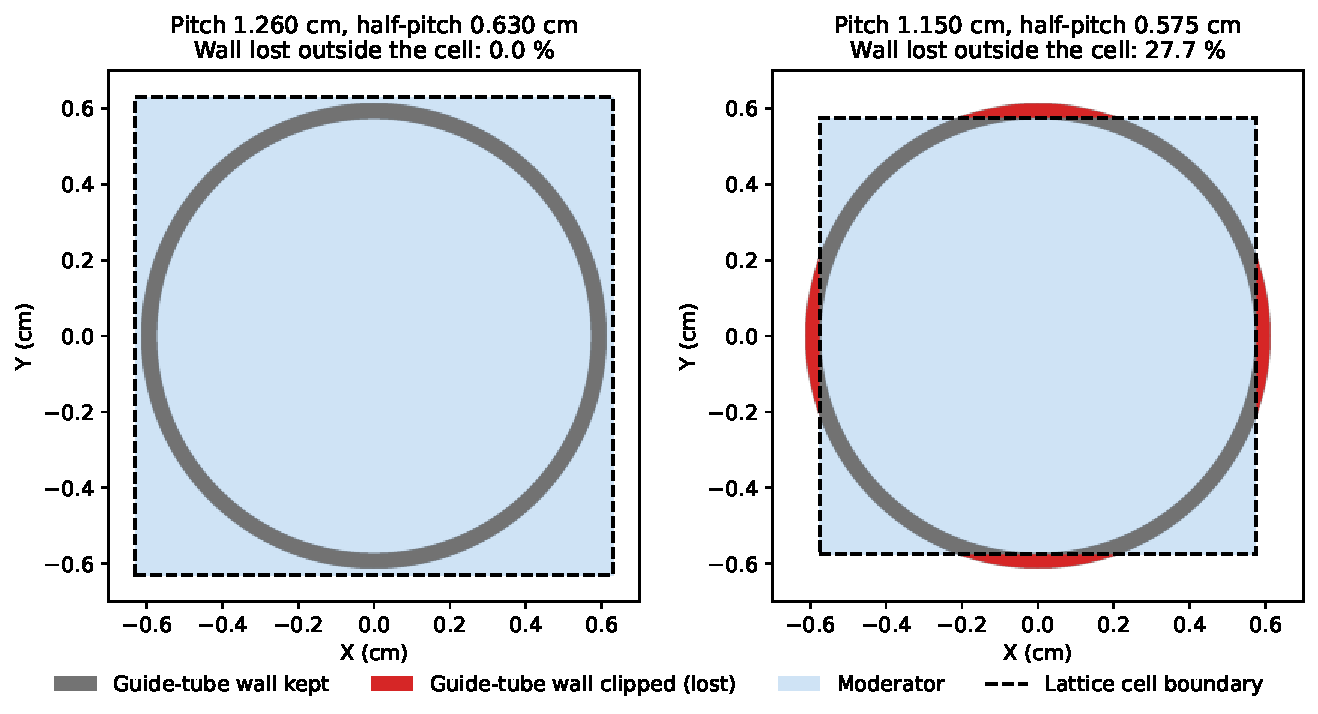
\includegraphics[width=0.75\linewidth]{images/th_gt_clip.pdf}
  \caption{Lattice cell: guide-tube wall at the reference pitch and at the lower pitch bound.}
  \label{fig:gt-clip}
\end{figure}

          \item The pitch is the design variable with the largest
                effect on the regulating-bank worth
                (Section~\ref{sec:res-c7-worth}).

          \item The pitch determines the moderator-to-fuel ratio, on which the
                moderator temperature coefficient
                depends~\cite{duderstadt_hamilton_1976}, and the coolant
                flow area and pressure drop~\cite{todreas_kazimi_2012}.
                The model has no thermal-hydraulic feedback, so it cannot
                itself show whether a given pitch is coolable. The pitch
                is therefore fixed at \SI{1.26}{cm}, whose thermal-hydraulic
                performance over the enrichment range searched here is
                demonstrated by decades of service in commercial
                PWRs and documented in their
                safety analysis
                reports~\cite{epr_fsar_ch4,todreas_kazimi_2012}.
        \end{itemize}

  \item The 2 assembly enrichment zones collapse to one variable,
        since the core-level enrichment variation comes entirely from
        the ring multipliers of Section~\ref{sec:meth-zoning}. Its
        upper bound is \SI{13.913}{wt\%}, the value that holds the
        as-built peripheral ring at its own limit through
        Equation~\eqref{eq:leu-box}, so no proposed design can violate
        $g_\mathrm{enr}$.

  \item The vessel-fit constraint reserves a clearance
        $c_\mathrm{v} = \SI{7.08}{cm}$ for a core barrel and a
        downcomer: the \SI{5.08}{cm} stainless steel barrel of the
        reference specification and a \SI{2.0}{cm} downcomer, adopted
        as a minimum coolant return path. The clearance acts on the
        geometric constraint alone, since the campaign transport model
        keeps a vacuum boundary at the reflector surface
        (Section~\ref{sec:meth-barrel}).

  \item The reflector thickness is limited by the radial budget that
        remains, Equation~\eqref{eq:refl-budget-c8}.
\end{enumerate}

\begin{equation}
t_\mathrm{refl}^{\max} = R_\mathrm{v} - c_\mathrm{v} - R_\mathrm{env}(p) - \delta
\label{eq:refl-budget-c8}
\end{equation}

\noindent where the symbols have the following meaning.

\begin{itemize}
  \item $t_\mathrm{refl}^{\max}$ is the largest reflector thickness that
        fits, \SI{5.669}{cm}, with an upper limit of \SI{5.66}{cm} in the design space so that the edge of the design space is strictly feasible.

  \item $R_\mathrm{v}$ is the vessel internal radius, \SI{90}{cm}.

  \item $c_\mathrm{v}$ is the reserved clearance, \SI{7.08}{cm}.

  \item $R_\mathrm{env}(p)$ is the circumscribed radius of the
        32-assembly fuel envelope at pitch $p$, \SI{77.231}{cm} at
        \SI{1.26}{cm}.

  \item $\delta$ is the radial tolerance, \SI{0.02}{cm}.
\end{itemize}

Fixing the pitch has a cost that was known before the campaign, since
the designs of lowest peaking in Campaign 7 reach it with thick
reflectors that fit only at a narrow pitch and cannot be built at \SI{1.26}{cm} (Section~\ref{sec:res-c8-intent}).

\subsection{Campaign 9 formulation}
\label{sec:meth-c9}

Campaigns 1 to 8 maximise the cycle length. In Campaign 8, every front
design has a cycle length well above the reported refuelling interval,
and the beginning-of-life excess reactivity that this cycle requires
can only be compensated at a large insertion depth of the regulating
banks
(Section~\ref{sec:res-c8-mission}). Campaign 9 therefore imposes the
required cycle length as a constraint and replaces it as an objective
by $c_\mathrm{max}$, the critical soluble boron concentration at the
reactivity maximum of the cycle. Minimising $c_\mathrm{max}$ directs the
search toward designs whose excess reactivity is compensated by the
burnable absorbers rather than by the coolant, so the objective
measures how far each design stands from soluble-boron-free operation.

Campaign 9 takes the five-year refuelling interval reported for LABGENE~\cite{dinizcosta_2017} as the mission requirement, which
gives the minimum cycle length of 1826 effective full power days used below.

\begin{equation}
\begin{aligned}
\min_{\mathbf{x}}\ &\big(F_{\Delta H}(\mathbf{x}),\ c_\mathrm{max}(\mathbf{x})\big) \\
\text{subject to}\ &\mathrm{EFPD}(\mathbf{x}) \ge 1826,\quad
F_{\Delta H}(\mathbf{x}) \le 1.65,\quad g_j(\mathbf{x}) \le 0
\end{aligned}
\label{eq:c9-problem}
\end{equation}

\noindent where the symbols have the following meaning.

\begin{itemize}
  \item $F_{\Delta H}$ is the radial peaking factor of the zoned core
        with all rods out at the beginning of life, the objective of
        Campaign 8, dimensionless.

  \item $c_\mathrm{max}$ is the critical boron concentration at the
        operating maximum of the reactivity history, in ppm, defined in
        Equation~\eqref{eq:c9-cmax}.

  \item $\mathrm{EFPD}$ is the cycle length of
        Section~\ref{sec:objective_functions}.

  \item $1.65$ is the peaking constraint, reduced from the exploratory
        bound of 2.0 of Table~\ref{tab:constraints} to the Technical
        Specification limit of 1.65 of a licensed pressurised water
        reactor~\cite{robinson_gd10}.

  \item $g_j$ are the constraints $g_{k\min}$, $g_{k\max}$,
        $g_\mathrm{enr}$ and $g_\mathrm{geom}$ of
        Table~\ref{tab:constraints} with their Campaign 8 values, the
        controllability constraint $g_\mathrm{ctrl}$ at beginning of life, and the
        same constraint evaluated at the operating maximum,
        $g_\mathrm{ctrl,peak}$.
\end{itemize}

The critical concentration is computed inside the evaluator from
unrodded core solves at \SI{1000}{ppm}, then at 2000 if $\rho(1000) > 0$
or at \SI{0}{ppm} otherwise, and at \SI{3000}{ppm} where the reactivity
has not yet changed sign. The beginning-of-life concentration
$c_\mathrm{BOL}$ is the root of $\rho(c)$, found by interpolation
over the interval between the 2 solves across which $\rho(c)$
changes sign, or by extrapolation above the highest,
and the differential worth is its local slope at that root. The
concentration at the operating maximum adds the part of the gadolinium
hump that the boron has to compensate, measured on the assembly depletion
history as a difference of reactivity.

\begin{equation}
\Delta\rho_\mathrm{hump} = \rho(k_\mathrm{peak}) - \rho(k_{\infty,\mathrm{BOL}}),
\qquad \rho(k) = 10^5\,\frac{k-1}{k}
\label{eq:c7-hump}
\end{equation}

\noindent where the symbols have the following meaning.

\begin{itemize}
  \item $\Delta\rho_\mathrm{hump}$ is the hump, in pcm. It is negative
        when the beginning of life is the most reactive state of the design.

  \item $k_{\infty,\mathrm{BOL}}$ is the assembly $k_\infty$ at zero burnup,
        xenon-free, at \SI{1000}{ppm}, dimensionless.

  \item $k_\mathrm{peak}$ is the largest assembly $k_\infty$ over the
        operating points of the depletion history after the beginning of
        life, dimensionless.

  \item $\rho$ is the reactivity, in pcm.
\end{itemize}

The concentration at the operating maximum is then obtained.

\begin{equation}
c_\mathrm{max} = c_\mathrm{BOL} + \frac{\max\!\big(L\,\Delta\rho_\mathrm{hump},\ 0\big)}{w_\mathrm{B}}
\label{eq:c9-cmax}
\end{equation}

\noindent where the symbols have the following meaning.

\begin{itemize}
  \item $c_\mathrm{BOL}$ is the critical boron concentration at
        beginning of life, in ppm.

  \item $\Delta\rho_\mathrm{hump}$ is the hump of
        Equation~\eqref{eq:c7-hump}, taken from the xenon-free assembly
        depletion history that the evaluator already computes, in pcm.
        A hump below \SI{400}{pcm} is set to zero. That threshold is twice
        the seed-to-seed standard deviation of the hump at the
        Campaign 9 transport setting of $4\,000\times60$, which the
        seed-replicated study of
        Section~\ref{sec:res-c9-dep-boron} measures at \SI{217}{pcm}, so a hump below it is not statistically significant in a single
        evaluation.

  \item $L$ is the ratio of the infinite multiplication factor of the assembly to the effective multiplication factor of the core, both at beginning of life, for the same design, which carries the assembly hump
        to the core, dimensionless.

  \item $w_\mathrm{B}$ is the differential boron worth at the root, in
        pcm per ppm.
\end{itemize}

Two guards bound the objective where the measurement cannot reach it:

\begin{itemize}
  \item \textbf{A design that cannot be made critical without boron
        returns a negative root:} it is clamped at \SI{0}{ppm}, since a
        minimised objective would otherwise rank it best. Such designs
        are infeasible on $g_{k\min}$ in any case.

  \item \textbf{A root above the highest measured concentration is
        extrapolated:} it is truncated at \SI{6000}{ppm}, twice that
        concentration. Boron self-shielding makes the true root higher
        than the linear extrapolation predicts, so a truncated design
        keeps its place at the bottom of the ranking of the evaluated designs.
\end{itemize}

\section{Leakage-corrected end-of-cycle criterion}
\label{sec:meth-ktarget}

The cycle length of every design is obtained from the depletion of a
single fuel assembly under reflective boundaries
(Section~\ref{sec:objective_functions}), which carries no leakage,
while the core of 32 assemblies loses neutrons through its radial
boundary and has a lower effective multiplication factor at the same fuel loading. The
size of that gap across the design space is measured in
Section~\ref{sec:res-kt-burnup}.

Placing the end of cycle where the assembly $k_\infty$ decreases to one
would therefore overestimate every cycle length, since the core would
have become subcritical long before. Depleting the full core in every
evaluation would remove the error at a cost the optimisation loop
cannot afford, so the correction is applied to the end-of-cycle
criterion and not to the depletion model. The core is critical when
$k_\mathrm{eff}^\mathrm{core} = 1$, so if the ratio of the assembly $k_\infty$ to the core $k_\mathrm{eff}^\mathrm{core}$ stays constant during burnup, the core reaches
criticality when the assembly $k_\infty$ has decreased to that ratio. That
ratio is the leakage-corrected $k_\mathrm{target}$ of Section~\ref{sec:bg-k}.

\begin{equation}
k_\mathrm{target}(p, t_\mathrm{refl})
= \frac{k_\infty^\mathrm{assembly}}{k_\mathrm{eff}^\mathrm{core}}
\label{eq:ktarget}
\end{equation}

\noindent where the symbols have the following meaning.

\begin{itemize}
  \item $k_\mathrm{target}$ is the leakage-corrected end-of-cycle multiplication factor entering Equation~\eqref{eq:eoc-k}, dimensionless.

  \item $k_\infty^\mathrm{assembly}$ is the infinite multiplication
        factor of the reflective single assembly, dimensionless.

  \item $k_\mathrm{eff}^\mathrm{core}$ is the effective multiplication
        factor of the two-dimensional 32-assembly core built with the
        same pitch and reflector thickness, dimensionless.

  \item $p$ is the pin pitch, in cm.

  \item $t_\mathrm{refl}$ is the reflector thickness, in cm.
\end{itemize}

One-group diffusion theory relates the two multiplication factors by
$k_\infty / k_\mathrm{eff} = 1 + M^2 B^2$, where $B^2$ is the geometric
buckling, in cm$^{-2}$, and $M^2$ the migration
area, in cm$^2$~\cite{duderstadt_hamilton_1976}. The two factors
depend on different quantities.

\begin{itemize}
  \item $B^2$ is determined by the size and the shape of the core
        alone. In this work, the pitch determines the width of the
        32-assembly array and the reflector thickness the distance over
        which the flux decays outside it, so the two geometric design
        variables act here, and the fuel does not.

  \item $M^2 = \tau + L^2$ is the mean square distance a neutron
        travels from birth to absorption, the Fermi age $\tau$ covering
        the slowing down and the diffusion area
        $L^2 = D / \Sigma_\mathrm{a}$ the thermal flight. This is where the fuel loading enters. A higher enrichment or a gadolinia
        loading raises the absorption cross section
        $\Sigma_\mathrm{a}$, which shortens $L^2$ and with it $M^2$, so the leakage penalty decreases.
\end{itemize}

Two consequences result, and both were tested in
Section~\ref{sec:res-kt-burnup}. Over burnup, the ratio is constant
within the Monte Carlo noise, with no drift being statistically significant at 2 standard
deviations, so one evaluation applies to the whole cycle. Across designs it
is not constant. The residual against the tabulated value is ordered by
enrichment and spans $+174$ to \SI{-329}{pcm}, which the same section
converts into a correction to the reported cycle length. The reference fuel loading has no gadolinia because the criterion is applied at the 
end of the cycle, where the gadolinium of every design has burnt out.

The ratio is therefore computed once, without depletion, at the beginning
of life on a reference assembly of fresh fuel at \SI{4.05}{wt\%} in
the outer zone and \SI{4.55}{wt\%} in the inner zone:

\begin{itemize}
  \item at each pitch, one solve of the reflective assembly gives
        $k_\infty^\mathrm{assembly}$,

  \item at each pair of pitch and reflector thickness, one solve of the
        two-dimensional core gives $k_\mathrm{eff}^\mathrm{core}$.
\end{itemize}

The reference fuel loading was fixed when the table was first
calibrated for Campaign 2, at the point where $k_\mathrm{target}$ first had to exist and before any campaign had returned a front to calibrate it on.
Its 2 enrichments sit inside commercial light water practice, below
the \SI{4.95}{wt\%} of the NuScale fuel design and the \SI{5}{wt\%}
that Section~\ref{subsec:comparison}
tabulates~\cite{nuscale_htp2_2017,iaea_smr_2024}, and it was not revised
once the campaigns began. Its error was measured a posteriori instead, in
Section~\ref{sec:res-kt-burnup}.

The $3\times7$ grid of Campaigns 2 to 7 required 3 assembly solves and
21 core solves. From Campaign 8 the pitch is fixed at \SI{1.26}{cm}, so
the table reduces to the 7 reflector thicknesses at that pitch, which
Campaign 9 reads as well. Inside the loop, $k_\mathrm{target}$ is
interpolated, so each evaluation needs only the depletion of its own
assembly. The constancy of the ratio with burnup was tested on ten
Campaign 8 designs (Section~\ref{sec:res-kt-burnup}), so the test covers
the table of Campaigns 8 and 9 and not the grid of Campaigns 2 to 7.

\subsection{Axial leakage factor and the three-dimensional \texorpdfstring{$k_\mathrm{target}$}{k-target}}
\label{sec:meth-lax}

The leakage-corrected $k_\mathrm{target}$ of Equation~\eqref{eq:ktarget} corrects the
infinite-lattice depletion for the radial leakage of the
two-dimensional core. The transport model has no axial extent, so the
axial leakage of the finite core is absent from every cycle length of
Campaigns 1 to 7, and a dedicated study in the post-analysis of
Campaign 7 measured it.

That study pairs each two-dimensional solve with a three-dimensional
one on the same seed. The three-dimensional model extends the core to a
finite active height of \SI{120}{cm} without structural components, adds
a \SI{15}{cm} slab of borated water above and below the fuel as the
axial reflector, a thickness assumed since no open source gives it for
LABGENE, and places a vacuum boundary beyond the slabs, with the radial reflector spanning the full height. Its
materials and zoned enrichment map are those of the Campaign 6
evaluator, which already uses the ring multipliers of Campaigns 8 and 9,
so the axial
extent is the only difference between the two models, and the ratio of their effective multiplication factors, $k_\mathrm{eff}^\mathrm{core,2D}/k_\mathrm{eff}^\mathrm{core,3D}$, isolates the axial leakage. Each paired
solve was executed at \num{150000} particles and 200 batches with 80 inactive,
in 2 seeds.

The axial leakage factor is the ratio of the two effective multiplication factors.

\begin{equation}
L_\mathrm{ax}(\mathbf{x}) = \frac{k_\mathrm{eff}^\mathrm{core,2D}(\mathbf{x})}{k_\mathrm{eff}^\mathrm{core,3D}(\mathbf{x})}
\label{eq:lax-def}
\end{equation}

\noindent where the symbols have the following meaning.

\begin{itemize}
  \item $L_\mathrm{ax}$ is the axial leakage factor, dimensionless.

  \item $k_\mathrm{eff}^\mathrm{core,2D}$ is the effective
        multiplication factor of the two-dimensional core of
        Equation~\eqref{eq:ktarget}, with the campaign radial reflector,
        dimensionless.

  \item $k_\mathrm{eff}^\mathrm{core,3D}$ is the effective
        multiplication factor of the same core at finite height with the
        axial reflectors, dimensionless.
\end{itemize}

The factor is measured at the end of this section. Its value,
$L_\mathrm{ax} = \num{1.0289}$, is applied to every design with a
systematic uncertainty of $\pm\SI{80}{pcm}$.

Campaigns 1 to 7 use the two-dimensional table. From Campaign 8, the axial factor multiplies $k_\mathrm{target}$, so that the end of cycle is defined on a finite-height core
from the start.

\begin{equation}
k_\mathrm{target}^\mathrm{3D}(t_\mathrm{refl}) = k_\mathrm{target}^\mathrm{2D}(t_\mathrm{refl}) \times L_\mathrm{ax}
\label{eq:ktarget-3d}
\end{equation}

\noindent where the symbols have the following meaning.

\begin{itemize}
  \item $k_\mathrm{target}^\mathrm{3D}$ is the value of $k_\infty$ that the depleting
        assembly must retain at the end of cycle for the finite core to be
        critical, dimensionless.

  \item $k_\mathrm{target}^\mathrm{2D}$ is the leakage-corrected $k_\mathrm{target}$ of
        Equation~\eqref{eq:ktarget} at the fixed pitch, dimensionless.

  \item $L_\mathrm{ax}$ is the axial factor, \num{1.0289}.

  \item $t_\mathrm{refl}$ is the reflector thickness, in cm.
\end{itemize}

Campaigns 8 and 9 fix the pitch at \SI{1.26}{cm}, which is not a grid
point of the table of Campaigns 2 to 7, whose pitches are 1.15, 1.29
and \SI{1.43}{cm}. Every leakage-corrected $k_\mathrm{target}$ read from
that table would therefore be interpolated between two pitches, and the
interpolation error would propagate into every cycle length. The
calibration of Section~\ref{sec:meth-ktarget} was therefore recomputed
at the fixed pitch, with one assembly solve and 7 core solves at
reflector thicknesses from 2.0 to \SI{5.66}{cm}. A weighted straight line
through those grid points replaces the raw values.

\begin{equation}
k_\mathrm{target}^\mathrm{2D}(t_\mathrm{refl}) = 1.054528 - 0.000516\, t_\mathrm{refl}
\label{eq:ktarget-c8-fit}
\end{equation}

The cycle lengths of Campaigns 8 and 9 therefore refer to a
finite-height core, and what the correction costs in cycle length are
reported in Section~\ref{sec:res-c8}.

\label{sec:res-c6-lax}

Table~\ref{tab:c6-lax} gives the factor for 6 designs chosen to span
the excess reactivity of the design space. Although their excess
reactivity ranges from \num{3863} to \SI{19593}{pcm}, a factor of 5, the axial leakage factor varies across them by only
\SI{157}{pcm}, with a standard deviation of \SI{72}{pcm} and no statistically significant correlation with the excess reactivity ($r = -0.55$, $p = 0.26$).
Its mean of \num{1.0289} is therefore applied as a constant from
Campaign 8.

\begin{table}[htbp]
  \centering
  \small
  \caption{Campaign 6, six designs: axial leakage factor.}
  \label{tab:c6-lax}
  \begin{tabular}{@{}lccccc@{}}
    \toprule
    Design & Excess reactivity & $k_\mathrm{eff}$, 2D & $k_\mathrm{eff}$, 3D &
      $\Delta k_\mathrm{axial}$ & $L_\mathrm{ax}$ \\
     & [pcm] & [--] & [--] & [pcm] & [--] \\
    \midrule
    C6-59 & \num{3863}  & 1.07088 & 1.04018 & 3070 & 1.02951 \\
    C6-22 & \num{6225}  & 1.09768 & 1.06638 & 3130 & 1.02935 \\
    C6-31 & \num{6722}  & 1.10226 & 1.07207 & 3020 & 1.02817 \\
    C6-69 & \num{8121}  & 1.12079 & 1.08839 & 3240 & 1.02977 \\
    C6-1  & \num{8163}  & 1.11990 & 1.08888 & 3101 & 1.02848 \\
    C6-86 & \num{19593} & 1.27869 & 1.24367 & 3502 & 1.02816 \\
    \midrule
    Mean  &              &         &         &      & 1.02891 \\
    \bottomrule
  \end{tabular}
\end{table}

\subsection{Axially resolved depletion}
\label{sec:meth-axial-dep}

Both leakage factors of $k_\mathrm{target}$ are measured on fresh fuel,
so the end-of-cycle criterion assumes that the axial power shape of
beginning of life persists over the cycle, which implies an axially
uniform burnup. The assumption is tested in the
post-analysis of Campaign 9 (Section~\ref{sec:res-c9-axial}) by
depleting the three-dimensional core model of
Section~\ref{sec:reactor-model} directly, with the active fuel cut into
$N$ axial layers of equal height, each carrying its own set of the 12 ring materials of the zoned core, so
that each layer burns in its own flux. With $N = 1$ the fuel is one material set over the full
\SI{120}{cm} and the burnup is axially uniform by construction. The end
of cycle of the layered core is defined relative to beginning of life,
so that the core loses the same reactivity as the assembly depleted in
the campaign.

\begin{equation}
k_\mathrm{EOC} = k_\mathrm{BOL}\,\frac{k_\mathrm{target}}{k_{\infty,\mathrm{BOL}}}
\label{eq:axial-eoc}
\end{equation}

\noindent where the symbols have the following meaning.

\begin{itemize}
  \item $k_\mathrm{EOC}$ and $k_\mathrm{BOL}$ are the effective
        multiplication factors of the core model at end of cycle and at
        beginning of life, dimensionless.
  \item $k_\mathrm{target}$ is the campaign value of the design,
        Equation~\eqref{eq:ktarget-3d}, dimensionless.
  \item $k_{\infty,\mathrm{BOL}}$ is the infinite multiplication factor of
        the design at beginning of life computed in the campaign,
        dimensionless.
\end{itemize}

If the leakage of the core
did not change with burnup, the layered core would reach
$k_\mathrm{EOC}$ at the burnup at which the assembly reaches
$k_\mathrm{target}$, and the 2 cycle lengths would coincide.

Because the one-layer and the eight-layer depletions of a design differ
only in the axial resolution of the burnup, the difference between
their histories of the effective multiplication factor quantifies the
axial burnup effect as a burnup-dependent correction to the axial
leakage factor.

\begin{equation}
\rho_A(B) = 10^5 \ln\!\left[\frac{k_1(B)/k_1(0)}{k_8(B)/k_8(0)}\right]
\label{eq:axial-rhoA}
\end{equation}

\noindent where the symbols have the following meaning.

\begin{itemize}
  \item $\rho_A(B)$ is the reactivity the axially resolved core loses
        beyond the uniform one at core-average burnup $B$, in pcm.
  \item $k_1(B)$ and $k_8(B)$ are the effective multiplication factors of
        the one-layer and the eight-layer core at that burnup,
        dimensionless.
  \item $L_\mathrm{ax}\exp(\rho_A/10^5)$ is the effective axial leakage
        factor at burnup $B$, dimensionless.
\end{itemize}

\section{Burnup limits in the simulations}
\label{sec:meth-atf}

Two assembly-average burnup limits act on the depletion of
Section~\ref{sec:bg-depletion}:

\begin{itemize}
  \item the discharge-burnup limit $B_\mathrm{burnup}$, which decides
        whether a design is acceptable,

  \item the depletion horizon $B_\mathrm{max}$, the burnup at which the
        depletion calculation is stopped.
\end{itemize}

The limit is $B_\mathrm{burnup} = \SI{55}{MWd/kgHM}$, the
assembly-average exposure limit of uranium dioxide in zirconium
cladding, set by cladding oxidation~\cite{song_sanchez_2026,alam_2019_hotchannel}.
The corresponding rod-average limit is \SI{62}{MWd/kgHM}. The limit is
applied at candidate selection to
the end-of-cycle burnups computed in the campaign, so it needs no new transport
calculation.

The horizon has changed with the campaigns:

\begin{itemize}
  \item \textbf{Campaign 1:} \SI{35.5}{MWd/kgHM}, the end of the fixed
        depletion schedule (Section~\ref{sec:res-hist-c1c2}).

  \item \textbf{Campaign 2:} \SI{100}{MWd/kgHM}, raised to test whether
        the censoring was an artefact of the stopping value
        (Section~\ref{sec:res-hist-c1c2}).

  \item \textbf{Campaigns 3 to 5:} \SI{75}{MWd/kgHM}, the value then
        adopted as the discharge limit
        (Sections~\ref{sec:res-hist-c3} and~\ref{sec:res-hist-c4c5}).

  \item \textbf{Campaigns 6 to 9:} $B_\mathrm{max} =
        \SI{100}{MWd/kgHM}$, well above the limit, so that designs reach
        the end-of-cycle multiplication factor $k_\mathrm{target}$
        before the depletion stops (Section~\ref{sec:res-hist-c6}).
\end{itemize}

\noindent With the horizon above the limit, right-censoring becomes
rare, and the objective surrogate is not trained on censored cycle
lengths. Its prediction is truncated at the horizon by
Equation~\eqref{eq:efpd-clip}.

\section{Moderator temperature coefficient and the MTC boron limit}
\label{sec:meth-mtc}

Because the boron concentration is fixed (Section~\ref{sec:meth-boron}),
the campaigns do not test whether a candidate can be kept critical by soluble boron at an
acceptable concentration. That concentration has an upper limit. A rise
in moderator temperature lowers the moderator density, and with it the
boron number density in the core, which inserts positive reactivity.
This contribution grows with the boron concentration, and above a
certain concentration the moderator temperature coefficient becomes
positive. A positive coefficient removes the negative temperature
feedback that stabilises the core against a power excursion, and it is
not acceptable at power. The concentration at which the coefficient is
zero is therefore the upper limit of the soluble boron, called here the
MTC boron limit, and it depends on the lattice.

\subsection{Definition and evaluation}
\label{sec:meth-mtc-def}

The coefficient is evaluated as a two-point difference at constant
pressure, with the moderator density taken consistently with the
temperature from the IAPWS-IF97 formulation~\cite{wagner_iapws_if97_2000}.

\begin{equation}
\alpha_\mathrm{M}(c) = \frac{\rho\!\left(T + \Delta T,\ c\right)
- \rho\!\left(T,\ c\right)}{\Delta T}
\label{eq:mtc}
\end{equation}

\noindent where the symbols have the following meaning.

\begin{itemize}
  \item $\alpha_\mathrm{M}$ is the moderator temperature coefficient, in
        pcm per K.
  \item $\rho$ is the core reactivity at the stated moderator temperature
        and soluble boron concentration, in pcm.
  \item $T$ is the moderator temperature, in K, with the density set from
        the steam tables at the operating pressure.
  \item $\Delta T$ is the temperature perturbation, in K.
  \item $c$ is the soluble boron concentration, in ppm.
\end{itemize}

The zero-coefficient concentration $c_\mathrm{MTC}$ is the root of
Equation~\eqref{eq:mtc} in concentration. It is obtained by a weighted
straight-line fit of the coefficient against concentration over the
3 scan points nearest the sign change, with the uncertainty
propagated from the fit covariance.

\begin{equation}
\alpha_\mathrm{M}\!\left(c_\mathrm{MTC}\right) = 0
\label{eq:ceiling}
\end{equation}

\noindent where $c_\mathrm{MTC}$ is the MTC boron limit, in ppm.

A design is acceptable on this criterion when its critical concentration
at the beginning of life, the root of the measured reactivity $\rho(c)$, or
its cycle maximum of Equation~\eqref{eq:c9-cmax} where a positive hump is statistically significant, does not exceed $c_\mathrm{MTC}$.

The limit is evaluated outside the optimisation loop, stored by the evaluator as $g_\mathrm{boron}$ and not imposed as a constraint. Each
scan solves the zoned core at 2 moderator temperatures and 4 boron
concentrations, with 2 seeds per point at $100\,000$ particles and 170
batches, on the three-dimensional core model of
Section~\ref{sec:reactor-model} with the control rods fully withdrawn
above the active core, so the limit and the three-dimensional
confirmation use the same geometry.

Two further rules apply to the limit:

\begin{itemize}
  \item \textbf{Extrapolation:} when the coefficient is still negative at
        \SI{3000}{ppm}, the highest concentration scanned, the limit is
        extrapolated from the fit.
  \item \textbf{Screen of Campaign 9:} one value, \SI{2763}{ppm}, applies
        to every design of the campaign. It is a two-point estimate of the
        three-dimensional limit of C8-47 at \SI{12.8}{MPa}, made before
        any lattice limit was measured.
\end{itemize}

Two temperature intervals were scanned, each centred on the average
coolant temperature of a reference plant:

\begin{itemize}
  \item 570 to \SI{590}{K} at \SI{15.5}{MPa}, centred on the moderator
        temperature of \SI{580}{K} of Table~\ref{tab:model-operating},
        with moderator densities of 0.733 and \SI{0.688}{g/cm^3}
        and saturation at \SI{617.9}{K}.
        These are the primary pressure and the average coolant
        temperature of a large pressurised water
        reactor~\cite{todreas_kazimi_2012,epr_fsar_ch4},

  \item 547 to \SI{567}{K} at \SI{12.8}{MPa}, centred on \SI{557}{K},
        with moderator densities of 0.771 and \SI{0.734}{g/cm^3}
        and saturation at \SI{602.8}{K}.
        These are the system pressure, \SI{12.76}{MPa}, and the core
        average temperature, \SI{557}{K}, of the NuScale
        module~\cite{nuscale_htp2_2017}.
\end{itemize}

The limit depends on the pressure through the moderator density. No
open source gives the primary conditions of LABGENE or of any naval
propulsion reactor, so the 2 intervals are reference points and carry
no claim about LABGENE.

The two-dimensional core omits the axial component of the moderator
feedback. When the moderator heats and expands, the axial leakage grows
and adds negative reactivity, so a limit evaluated in two dimensions
underestimates the three-dimensional one. The omitted term is the difference between the three- and
the two-dimensional coefficients at the same state, measured by a scan
of the same lattice on the two-dimensional core.

\begin{equation}
\alpha_\mathrm{ax} = \alpha_\mathrm{M}^\mathrm{3D} - \alpha_\mathrm{M}^\mathrm{2D}
\label{eq:axial-feedback}
\end{equation}

\noindent where $\alpha_\mathrm{ax}$ is the axial leakage contribution
and $\alpha_\mathrm{M}^\mathrm{3D}$ and $\alpha_\mathrm{M}^\mathrm{2D}$
are the moderator temperature coefficients in three and in two
dimensions, all in pcm per K. The two-dimensional limit is therefore
reported as a conservative bound and the three-dimensional limit as
the physical result.

\section{Transport fidelity and seeding}
\label{sec:meth-fidelity}

Every quantity returned by the evaluator is a Monte Carlo estimate,
and every one of them carries a statistical uncertainty set by the
number of neutron histories. The multiplication factor and the cycle length
are unbiased estimates, with an error symmetric about the true value
(Section~\ref{sec:bg-mc-stats})~\cite{lux_koblinger_1991}. The peaking
factor $F_{\Delta H}$ carries a positive bias on top of it, for the
reason given in Section~\ref{sec:meth-fdh}. Both the bias and the
variance decrease as the number of active histories grows, and the cost of
the solve grows with them.

Two settings of the transport solve therefore control the quality of
every result of this work.

\begin{itemize}
  \item \textbf{Fidelity:} the number of particles per batch and the
        number of active and inactive batches. It determines the relative standard error of every tally and the bias of the peaking
        estimator.

  \item \textbf{Seed policy:} the rule that assigns the initial seed of
        the pseudo-random number generator. It decides whether 2
        evaluations use the same random-number sequence, and
        with it whether their statistical noise is correlated.
\end{itemize}

The need to control both was established in Campaign 2
(Section~\ref{sec:res-c1c2}). In that campaign, at $4\,000\times60$ with
one shared seed, the error of the stored peaking values exceeded the
spread of the front, so the high-fidelity re-evaluation changed the order
of the candidates.

\subsection{Fidelity study}
\label{sec:meth-fid-ladder}

The fidelity of the high-fidelity search was chosen from a
seed-replicated study of the assembly estimator.
\label{sec:res-c3-fidelity}
The Campaign 2 front and the Campaign 3 candidates were repeated at
$4\,000$, $16\,000$, $64\,000$ and $256\,000$ particles with
independent seeds, so that the seed-to-seed standard deviation measures
the noise and the difference to the highest setting measures the bias.
Figure~\ref{fig:fid-ladder} and Table~\ref{tab:fid-ladder} give both at
each setting.

\begin{figure}[htbp]
  \centering
  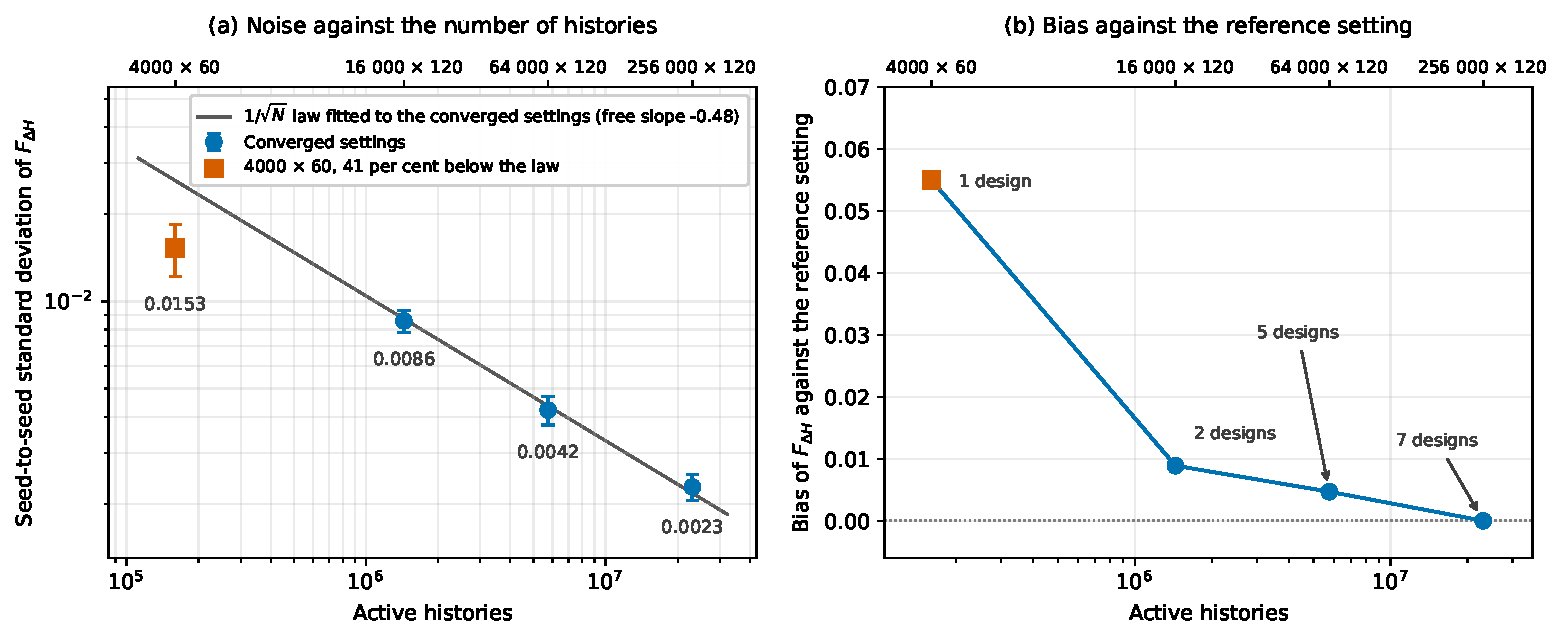
\includegraphics[width=\textwidth]{images/th_fid_ladder}
  \caption{Single assembly at beginning of life: noise and bias of the peaking estimator.}
  \label{fig:fid-ladder}
\end{figure}

Between $16\,000$ and $256\,000$ particles the noise decreases as the
$1/\sqrt{N}$ law of independent histories, at a fitted exponent of
$-0.48$, while the $4\,000$-particle setting is \SI{41}{\%} below
that law, because at that count the estimator is biased rather than
merely noisy. The step to $16\,000\times120$ multiplies the active
histories by nine, from \num{160000} to \num{1440000}, and removes most
of that bias, and each further factor of 4 halves the noise at 2.5
to 3.7 times the wall time, which is why $16\,000\times120$ was adopted
for the high-fidelity search of Campaigns 3 and 5.
The reference setting itself retains a residual bias of about
$+0.005$, so the bias of the table is relative to it and not to the
true value.

\begin{table}[htbp]
  \centering
  \begin{threeparttable}
  \caption{Single assembly at beginning of life: fidelity study of the peaking estimator.}
  \label{tab:fid-ladder}
  \small
  \setlength{\tabcolsep}{4pt}
  \begin{tabular}{@{}lcccccc@{}}
    \toprule
    Particles $\times$ batches & Active histories & Designs & $s_F$\tnote{a} & $\varepsilon_\mathrm{hot}$\tnote{b} & Bias\tnote{c} & Wall time (s) \\
    \midrule
    $4\,000\times60$ (20)    & $1.6\times10^{5}$  & 3  & 0.0153 & 3.6\%  & $+0.055$ (1)  & not stored \\
    $16\,000\times120$ (30)  & $1.44\times10^{6}$ & 17 & 0.0086 & 1.10\% & $+0.0089$ (2) & 19.3 \\
    $64\,000\times120$ (30)  & $5.76\times10^{6}$ & 10 & 0.0042 & 0.57\% & $+0.0047$ (5) & 48.3 \\
    $256\,000\times120$ (30) & $2.30\times10^{7}$ & 7  & 0.0023 & 0.29\% & reference     & 177.5 \\
    \bottomrule
  \end{tabular}
  \begin{tablenotes}[flushleft]\footnotesize
    \item Inactive batches in parentheses.
    \item[a] Seed-to-seed standard deviation of $F_{\Delta H}$, pooled
      over the designs of the setting.
    \item[b] Relative standard error of the hottest-pin tally, mean over
      the calculations of the setting.
    \item[c] Mean over designs of the difference between the setting mean
      and the $256\,000\times120$ mean of the same design. The number of
      designs with a reference solve is in parentheses.
  \end{tablenotes}
  \end{threeparttable}
\end{table}

A second study measures the core estimator. The study of
Table~\ref{tab:fid-ladder} covers the assembly estimator, which is the
peaking objective of Campaigns 1 to 3, while from Campaign 4 the
objective is the core estimator at $100\,000\times170$ (60 inactive),
whose maximum is taken over the pins of the zoned 32-assembly core. Its
bias is taken against the extrapolation of each design to an infinite
number of histories.

\begin{equation}
F_{\Delta H}(N) = F_\infty + \frac{a}{\sqrt{N}}
\label{eq:fdh-extrap}
\end{equation}

\noindent where $F_{\Delta H}(N)$ is the mean over the seeds of the core
peaking factor at $N$ active histories, the particles per batch
multiplied by the 110 active batches, $F_\infty$ is the extrapolated
value, and $a$ is the fitted bias coefficient, all dimensionless. The
extrapolation assumes that the bias decreases as $1/\sqrt{N}$. The study
that applies it is reported in Section~\ref{sec:res-c9-peaking}.

A third study measures the depletion that gives the cycle length. The
assembly depletion of the five Campaign 9 front designs was repeated
with independent seeds at the setting of the search, 4 to 8
replicates per design, and once at $16\,000\times120$. The replicates
measure the seed-to-seed error of the cycle length, and the
high-fidelity depletion measures the shift between the 2 settings, which
the two-tier strategy of Section~\ref{sec:meth-fid-settings} assumes to
be zero. The study is reported in Section~\ref{sec:res-c9-dep-check}.

All three studies repeat each solve with independent seeds, and the
replicates also define how two estimates are compared. Wherever 2 designs, or one design at 2
settings, are compared in Chapter~\ref{ch:results}, the comparison is
the two-sample statistic of Section~\ref{sec:bg-mc}, $t$, computed from
the seed-replicated means and their standard errors, with
$|t| \approx 2$ as the separation threshold.

\subsection{Transport settings per campaign}
\label{sec:meth-fid-settings}

Table~\ref{tab:fidelity} lists the transport settings of every campaign.
A campaign row gives the assembly depletion of each evaluation, and the
other rows give the calculations executed in addition to it. The settings
are stored in each campaign checkpoint and cannot change during a
campaign.

\begin{table}[htbp]
  \centering
  \begin{threeparttable}
  \caption{Campaigns 1 to 9: transport settings per campaign and per evaluation stage.}
  \label{tab:fidelity}
  \footnotesize
  \begin{tabularx}{\textwidth}{@{}>{\raggedright\arraybackslash}p{0.21\textwidth}c>{\raggedright\arraybackslash}p{0.17\textwidth}>{\raggedright\arraybackslash}X@{}}
    \toprule
    Stage & Particles $\times$ batches\tnote{a} & Seed policy & Role \\
    \midrule
    Campaign 1     & $4\,000\times60$ (20)    & shared              & verification \\
    Campaign 2     & $4\,000\times60$ (20)    & shared              & low-fidelity search \\
    Campaign 3     & $16\,000\times120$ (30)  & per-design          & high-fidelity search \\
    C4 core solve  & $100\,000\times170$ (60) & per-design, salted  & core solve: $F_{\Delta H}$ \\
    Campaign 5     & $16\,000\times120$ (30)  & per-design          & high-fidelity search \\
    C5 core solve  & $100\,000\times170$ (60) & per-design, salted  & core solve: $F_{\Delta H}$ \\
    Campaign 6     & $4\,000\times60$ (20)    & per-design          & low-fidelity search \\
    C6 core solve  & $100\,000\times170$ (60) & per-design, salted  & core solve: $F_{\Delta H}$, $k$ window \\
    Campaign 7     & $4\,000\times60$ (20)    & per-design          & low-fidelity search \\
    C7 core solves & $100\,000\times170$ (60) & per-design, salted  & core solves: $F_{\Delta H}$, $k$ window, one rodded solve \\
    Campaign 8     & $4\,000\times60$ (20)    & per-design          & low-fidelity search \\
    C8 core solves & $100\,000\times170$ (60) & per-design, salted  & core solves: $F_{\Delta H}$, $k$ window, 2 rodded solves \\
    Campaign 9     & $4\,000\times60$ (20)    & per-design          & low-fidelity search \\
    C9 core solves & $100\,000\times170$ (60) & per-design, salted  & core solves: as C8, and unrodded at 0, 2000 or 3000\,ppm for $c_\mathrm{max}$ \\
    Preselection   & $64\,000\times120$ (30)  & replicated          & selection, first stage \\
    Confirmation   & $256\,000\times120$ (30) & replicated, 8 seeds & selection, second stage \\
    \bottomrule
  \end{tabularx}
  \begin{tablenotes}[flushleft]\footnotesize
    \item[a] Inactive batches in parentheses.
  \end{tablenotes}
  \end{threeparttable}
\end{table}

From Campaign 6, the assembly depletion returns to $4\,000\times60$,
the setting of Campaigns 1 and 2, after the $16\,000\times120$ of
Campaigns 3 and 5. The change is part of a two-tier fidelity strategy:

\begin{itemize}
  \item \textbf{Search:} executed at low fidelity, where it needs many
        evaluations.
  \item \textbf{Core solves:} inside each evaluation, they evaluate
        $F_{\Delta H}$, the reactivity window and the controllability
        constraints, and stay at $100\,000\times170$.
\end{itemize}

The fidelity is kept constant across all blocks of a campaign, because
a surrogate trained on mixed-fidelity data has a bias that changes with
the evaluation date and cannot be corrected a posteriori.

The post-analysis of Campaigns 8 and 9 is executed outside the loop, on
the designs the 2 campaigns evaluated, and Table~\ref{tab:fidelity-post}
lists its stages.

\begin{table}[!htb]
  \centering
  \begin{threeparttable}
  \caption{Post-analysis of Campaigns 8 and 9: transport settings per stage.}
  \label{tab:fidelity-post}
  \footnotesize
  \begin{tabularx}{\textwidth}{@{}>{\raggedright\arraybackslash}p{0.21\textwidth}c>{\raggedright\arraybackslash}p{0.17\textwidth}>{\raggedright\arraybackslash}X@{}}
    \toprule
    Stage & Particles $\times$ batches\tnote{a} & Seed policy & Role \\
    \midrule
    Paired 2D and 3D core solves & $150\,000\times200$ (80) & replicated, 2 seeds & three-dimensional confirmation of the C8 candidates, the C9 front and the continuation front \\
    C8 boron solves & $150\,000\times200$\tnote{b} & one seed & boron worth and critical concentration \\
    C8 leakage-factor study & $60\,000\times170$\tnote{b} & one seed & leakage factor against enrichment and reflector thickness \\
    MTC scans & $100\,000\times170$ (60) & replicated, 2 seeds & MTC boron limit of C8-47 and of 11 C9 lattices \\
    C9 core fidelity study & $25\,000$ to $400\,000\times170$ (60) & replicated, 8 seeds & bias of the core peaking estimator \\
    C9 depletion replicates & $4\,000\times60$ (20) & salted, 4 to 8 per design & seed-to-seed error of the cycle length \\
    C9 high-fidelity depletion & $16\,000\times120$ (30) & campaign seed & fidelity shift of the cycle length \\
        C9 core depletions & $20\,000\times160$ (60) & salted & zoned 2D and axially layered 3D depletion, 4 further seeds on 3 designs \\
    C9 rod-count study & $4\,000\times60$ (20), $20\,000\times160$ (60) & per-design, salted & 5 lattices at one gadolinia inventory, evaluated and depleted in 8 layers \\
    C9 predicted front & $4\,000\times60$ (20) & per-design & transport evaluation of the 6 designs of the surrogate front \\
    \bottomrule
  \end{tabularx}
  \begin{tablenotes}[flushleft]\footnotesize
    \item[a] Inactive batches in parentheses.
    \item[b] Number of inactive batches not stored with the results.
  \end{tablenotes}
  \end{threeparttable}
\end{table}

Two stages of Table~\ref{tab:fidelity-post} give most of the results of
the post-analysis: the paired two- and three-dimensional core solves at
$150\,000\times200$, which confirm the candidates of Campaign 8 and the
front of Campaign 9 (Sections~\ref{sec:res-c8-split}
and~\ref{sec:res-c9-ctrl3d}), and the core depletions of Campaign 9 at
$20\,000\times160$, in two dimensions with the zoning and in three with
axial layers (Section~\ref{sec:res-c9-axial}).


\subsection{Seed policy}
\label{sec:meth-fid-seed}

OpenMC initialises its pseudo-random number generator with the same
default seed in every calculation unless another seed is set. With that
default, every design is computed on the same random-number sequence.
Two similar problems computed on one sequence consume the same random
numbers at the same points of each history, so the source sites and
the interaction outcomes they sample coincide until the two models
differ. Their tally errors then share a common component and the noise
of different designs is positively correlated, which is the mechanism
of correlated sampling~\cite{lux_koblinger_1991}.

The coupling is partial
here, because 2 designs differ in geometry and fuel loading and their
histories diverge as soon as that difference changes a sampled
interaction. Campaigns 1 and 2 were executed on that default seed, so every
design of both campaigns shared one sequence. The effect was detected
in Campaign 2, where evaluating the finalists again at high fidelity with independent seeds did not preserve their ranking
(Section~\ref{sec:res-c1c2}).

From Campaign 3, each design receives its own seed, a CRC32 hash of its
design vector. Each core solve adds a fixed string to the hash, the
salt, so that the assembly and core solves of one design are also executed on
different sequences. The policy has two properties.

\begin{itemize}
  \item \textbf{Reproducibility:} the seed depends only on the design,
        so repeating an evaluation reproduces its beginning-of-life
        solves.

  \item \textbf{Independent noise:} the noise of 2 designs is
        uncorrelated, which is the independent and identically
        distributed noise assumed by the white-noise term of the
        Gaussian-process kernel of Section~\ref{sec:bg-gp}.
\end{itemize}

The seed fixes the beginning-of-life solves of a design, and it does
not fix its depletion. Whether the depletion is reproduced was tested
by repeating the assembly depletion of the five Campaign 9 front
designs with the campaign seed. The cycle lengths differ from the
campaign values by $-76$ to \SI{+5}{d}, within 2.6 times the
seed-to-seed standard deviation of \SI{29.1}{d}
(Section~\ref{sec:res-c9-dep-error}), so the repetition reproduces the
depletion only within its statistical error. A thread test on C9-47 gives
the cause. On one thread two executions with the same seed are
bit-identical, while on 64 threads they differ by \SI{669}{pcm} at the
second depletion step, because the threads accumulate the tallies in a
different order and round the reaction rates passed to the depletion
solver differently.

Each replicate and each core depletion of the post-analysis takes its
seed from the same hash with a salt of its own, so every replicate is
computed on an independent random-number sequence and counts as an
independent sample together with the campaign evaluation.

%% labels of the removed section, kept so that the cross-references still resolve
\label{sec:meth-cycle-error}\label{sec:meth-stats}\label{eq:noise-margin-set}

\section{Surrogate-assisted active-learning loop}
\label{sec:meth-loop}

The loop is described in Section~\ref{sec:bg-al} and
Figure~\ref{fig:bg-al}. It starts from a Latin-hypercube design of
experiments, and each iteration then has 3 steps.

\begin{enumerate}
  \item Gaussian-process surrogates of the objectives and the
        constraints (Section~\ref{sec:bg-gp}).

  \item An NSGA-II search on the surrogates
        (Section~\ref{sec:bg-nsga2}).

  \item An infill batch evaluated with OpenMC.
\end{enumerate}

The design of experiments holds 6 to 9 points per design variable, 24
to 42 points in all. The literature gives three recommendations for its
size, with $n_x$ the number of design variables:

\begin{itemize}
  \item \textbf{Lower limit:} a benchmark of Bayesian optimisation finds
        no drawback in initial designs as small as $n_x + 4$ points, with
        $7.5\,n_x$ as its default~\cite{leriche_picheny_2021}.
  \item \textbf{Upper limit:} the rule of thumb for the initial design of a
        Gaussian-process surrogate is 10 points per
        variable~\cite{whyte_2020}.
  \item \textbf{Budget share:} surrogate-based optimisation places $1/3$
        of the evaluation budget in the sampling plan and $2/3$ in
        infill~\cite{forrester_book_2008}.
\end{itemize}

The size was chosen as a compromise between the computation time, at 10
to 25 minutes per transport evaluation, and the range of these
recommendations, with no fewer than 6 points per variable.

The design of experiments is sampled over the bounds of the design
space before any design is evaluated. Two constraints act on it, the
enrichment limit, written into the bounds
(Section~\ref{sec:meth-zoning-box}), and the vessel fit
$g_\mathrm{geom}$, which is analytic, so the sampler keeps only the
points that satisfy it. Every other constraint enters the loop through
its surrogate and acts on the infill selection alone.

This section fixes what Chapter~\ref{ch:background} leaves open.

\begin{enumerate}
  \item The stopping rule.

  \item The settings with which the loop was executed.

  \item The acquisition function, with the 3 revisions that
        Campaign 6 made necessary.
\end{enumerate}

Figure~\ref{fig:meth-loop-flow} summarises one iteration as
implemented.

\begin{figure}[htbp]
  \centering
  \resizebox{\textwidth}{!}{%
  \begin{tikzpicture}[
      box/.style={draw, rounded corners=2pt, align=center, font=\small,
                  text width=2.35cm, minimum height=1.35cm, fill=blue!6},
      outbox/.style={box, fill=green!10},
      arr/.style={-{Stealth[length=2.2mm]}, thick},
      node distance=0.45cm]
    \node[box] (a) {Designs evaluated with OpenMC};
    \node[box, right=of a] (b) {Fit one GP per objective and constraint};
    \node[box, right=of b] (c) {NSGA-II on the surrogates, $300\times400$};
    \node[box, right=of c] (d) {Rank-1 candidate set};
    \node[box, right=of d] (e) {Acquisition: infill batch of 6};
    \node[box, right=of e] (f) {OpenMC evaluation and checkpoint};
    \node[outbox, right=1.7cm of f] (g) {Pareto front of the evaluated designs};
    \draw[arr] (a) -- (b);
    \draw[arr] (b) -- (c);
    \draw[arr] (c) -- (d);
    \draw[arr] (d) -- (e);
    \draw[arr] (e) -- (f);
    \draw[arr] (f) -- node[above, font=\footnotesize, align=center] {Rule\\satisfied} (g);
    \draw[arr] (f.south) -- ++(0,-0.55) -| node[pos=0.25, below, font=\footnotesize]
      {Stopping rule not satisfied: next iteration} (a.south);
  \end{tikzpicture}}
  \caption{Surrogate-assisted loop: one iteration.}
  \label{fig:meth-loop-flow}
\end{figure}

\subsection{Stopping rule}
\label{sec:meth-loop-stop}

The loop stops when two conditions hold together. The first uses the
relative gain of the hypervolume of Section~\ref{sec:bg-hv} in each
iteration.

\begin{equation}
\Delta_t = \frac{H_t - H_{t-1}}{H_{t-1}}
\label{eq:hv-stop}
\end{equation}

\noindent where $\Delta_t$ is the relative gain of iteration $t$,
dimensionless, and $H_t$ and $H_{t-1}$ are the hypervolumes of the evaluated designs after iterations $t$ and $t-1$, Equation~\eqref{eq:hv}, against
the fixed reference point. The condition is that the gain stays below
one per cent in each of the last 3 iterations:

\begin{equation}
\Delta_{T-2} < 0.01, \qquad \Delta_{T-1} < 0.01, \qquad \Delta_{T} < 0.01
\label{eq:hv-stop-cond}
\end{equation}

\noindent where $T$ is the last iteration completed.

The second condition is that no censored design remains on the Pareto
front, since a censored cycle length is only a lower bound. A three-iteration window is
used because the gains are not monotonic.

The rule is necessary and not sufficient, because the hypervolume also
stops growing when the acquisition selects designs almost identical to
those already evaluated, or infeasible ones
(Section~\ref{sec:res-c6-margin}). Two health indicators are therefore computed at every iteration and
checked before the rule is accepted:

\begin{itemize}
  \item the number of candidates that pass the feasibility margin of
        Equation~\eqref{eq:feas-margin}, which shows whether the
        constraint surrogate is still changing,

  \item the depth of the separation relaxation of
        Section~\ref{sec:meth-acq}, which shows whether the surrogate
        front still contains new designs.
\end{itemize}

\subsection{Surrogate and loop settings}
\label{sec:meth-loop-settings}

The inputs and outputs of every Gaussian process are standardised, so
that one dimensionless length-scale per variable of
Equation~\eqref{eq:kernel-r} is meaningful.

\begin{equation}
z_d = \frac{x_d - \bar{x}_d}{s_d}
\label{eq:standardise}
\end{equation}

\noindent where $z_d$ is the standardised value of variable $d$,
dimensionless, and $\bar{x}_d$ and $s_d$ are the mean and the standard
deviation of that variable over the training data, in its native unit. The
outputs are standardised in the same way.

One independent Gaussian process with the kernel of
Equation~\eqref{eq:kernel} is fitted to each output, the two objectives
and every constraint that is not computed analytically. Its
hyperparameters are refitted on all the training data by maximising the log
marginal likelihood~\cite{rasmussen_gp_2006}. The refit is performed
once per iteration of the active-learning loop, that is once the
OpenMC evaluations of an infill batch have entered the training data. The
generations of the NSGA-II search are executed on surrogates whose
hyperparameters are kept fixed and are not refitted.

\begin{equation}
\log p(\mathbf{y} \mid \boldsymbol{\theta})
= -\tfrac{1}{2}\,\mathbf{y}^{\mathsf T}
\left( \mathbf{K} + \sigma_n^{2}\mathbf{I} \right)^{-1} \mathbf{y}
- \tfrac{1}{2} \log \left| \mathbf{K} + \sigma_n^{2}\mathbf{I} \right|
- \tfrac{n}{2} \log 2\pi
\label{eq:gp-lml}
\end{equation}

\noindent where $\boldsymbol{\theta} = (\ell_1, \dots, \ell_D,
\sigma_f, \sigma_n)$ is the vector of hyperparameters, and the other
symbols are those of Equations~\eqref{eq:kernel} to~\eqref{eq:gp-var}.
The maximisation is restarted from 4 random starting points to avoid
a local maximum. The first term rewards the fit to the training data and the
second penalises model complexity, so the fitted length-scales do not
simply interpolate the noise.

Table~\ref{tab:loop-settings} gives the loop settings of Campaigns 3
to 9. Campaign 3 is the first campaign in which per-design seeding made the evaluated designs statistically consistent.

\begin{table}[htbp]
  \centering
  \small
  \caption{Loop settings per campaign.}
  \label{tab:loop-settings}
  \begin{tabular}{@{}lccccl@{}}
    \toprule
    Campaign & Initial designs & Batch & Iterations & Total & End \\
    \midrule
    C3 & 36 & 6 & 6  & 72  & stopping rule satisfied \\
    C4 & 36 & 6 & 3  & 54  & -- \\
    C5 & 42 & 6 & 3  & 60  & -- \\
    C6 & 42 & 6 & 12 & 114 & stopping rule satisfied \\
    C7 & 42 & 6 & 3  & 60  & -- \\
    C8 & 36 & 6 & 4  & 60  & -- \\
    C9 & 24 & 6 & 6  & 60  & -- \\
    \bottomrule
  \end{tabular}
\end{table}

\subsection{Acquisition function}
\label{sec:meth-acq}

The infill batch is selected from the rank-1 set of the final NSGA-II
population on the surrogates. The base criterion, whose steps are
listed in Section~\ref{sec:bg-al}, ranks the candidates by their
aggregated predictive uncertainty.

\begin{equation}
a_i \;=\; \sum_{m=1}^{2} \frac{\sigma_{im}}{\max_{l}\,\sigma_{lm}}
\label{eq:acq-score}
\end{equation}

\noindent where the symbols have the following meaning.

\begin{itemize}
  \item $a_i$ is the acquisition score of candidate $i$, dimensionless.
  \item $\sigma_{im}$ is the posterior standard deviation of objective
        $m$ at candidate $i$, Equation~\eqref{eq:gp-var}.
  \item $\max_l \sigma_{lm}$ is the largest posterior standard deviation
        of objective $m$ over the same rank-1 candidate set, so each term
        of the sum is between zero and one.
\end{itemize}

The normalisation is per objective, since the two are measured
in different units and the larger of them would otherwise set the
ranking on its own. This is a pure exploration criterion in the sense
of~\cite{forrester_book_2008}.

Campaign 6 exposed three failures of the base criterion, and each was
corrected by one revision, introduced one per block so that each effect
is attributable, as the test at the end of this section shows.
Figure~\ref{fig:meth-acq-flow} shows the resulting selection.

\begin{itemize}
  \item \textbf{Horizon-aware surrogate objective:} the problem is
        extrapolation beyond the depletion horizon. The OpenMC
        evaluator stops every depletion at $B_\mathrm{max}$, so a
        design that has not reached $k_\mathrm{target}$ is stored with the
        cycle length it had at the horizon. That value is a lower bound
        on the cycle length the design would have reached, since its
        depletion was stopped before $k_\mathrm{target}$. The Gaussian
        process, trained on these lower bounds, predicts cycle lengths
        above the horizon, and the search concentrates on designs whose
        predicted value the evaluator cannot return. The surrogate objective is truncated at the horizon
        before it enters the search.

        \begin{equation}
        \tilde{f}_1(\mathbf{x}) \;=\;
        \max\!\left( f_1(\mathbf{x}),\; -E_\mathrm{max} \right),
        \qquad
        E_\mathrm{max} \;=\; \frac{1000\, B_\mathrm{max}}{P_\mathrm{spec}}
        \label{eq:efpd-clip}
        \end{equation}

        \noindent where the symbols have the following meaning.

        \begin{itemize}
          \item $\tilde{f}_1$ and $f_1$ are the truncated and the raw
                predictions of the first objective in minimisation form,
                the negative cycle length, in days.
          \item $E_\mathrm{max}$ is the horizon expressed as a cycle
                length, \num{10016.7} days at
                $B_\mathrm{max} = \SI{100}{MWd/kgHM}$.
          \item $P_\mathrm{spec}$ is the specific power of
                Table~\ref{tab:model-operating}.
        \end{itemize}

        The designs predicted beyond the horizon share one truncated
        value, so non-dominated sorting ranks them by peaking alone, as
        the constrained-domination principle ranks censored
        designs~\cite{deb_nsga2_2002}.

  \item \textbf{Feasibility margin:} the base criterion of
        Equation~\eqref{eq:acq-score} uses only the objective
        surrogates, so it ignores the constraints. Far from the training
        designs, beyond the kernel length-scales $\ell_d$, the posterior
        mean of Equation~\eqref{eq:gp-mean} returns to the prior mean,
        the average of the training data, so a constraint surrogate
        predicts a value typical of the evaluated designs even where the
        constraint is violated, and the mean alone would admit such
        designs as feasible. The posterior standard deviation is large in
        those regions, so every candidate is scored on
        the constraint surrogates with an uncertainty margin.

        \begin{equation}
        s_i \;=\; \max_{j \,\in\, \mathcal{G}_\mathrm{GP}}
        \left( \mu_{ij} + \kappa\,\sigma_{ij} \right)
        \label{eq:feas-margin}
        \end{equation}

        \noindent where the symbols have the following meaning.

        \begin{itemize}
          \item $s_i$ is the margin score of candidate $i$, in the
                normalised constraint units of
                Equation~\eqref{eq:cv-norm}.
          \item $\mathcal{G}_\mathrm{GP}$ is the set of constraints
                predicted by a surrogate.
          \item $\mu_{ij}$ and $\sigma_{ij}$ are the posterior mean and
                standard deviation of constraint $j$.
          \item $\kappa$ is the margin factor, 1.5, the value stored for
                the last Campaign 6 session and used in Campaigns 8 and 9.
        \end{itemize}

        The candidates are then ordered in two tiers:
        \begin{enumerate}
          \item \textbf{Margin-feasible candidates:} those with
                $s_i \le 0$, ranked first by descending exploration
                score $a_i$ of Equation~\eqref{eq:acq-score}.
          \item \textbf{Fallback ordering:} the remaining candidates,
                with $s_i > 0$, ordered by ascending $s_i$, the least
                likely to violate a constraint first. It is the ordering
                the selection falls back on when too few candidates are
                margin-feasible to fill the batch.
        \end{enumerate}
        The batch is therefore always filled with the least risky
        designs. The margin applies the rule of safe Bayesian
        optimisation, which admits a point only where the confidence
        bound of every constraint is satisfied~\cite{sui_safeopt_2015},
        and it is the deterministic counterpart of the
        probability-of-feasibility weighting~\cite{forrester_book_2008}.
        Its effect on Campaign 6 is reported at the end of this section.

  \item \textbf{Batch diversity:} batch collapse is an infill batch
        whose designs are almost identical, so several transport
        evaluations are spent on one region of the design space. It
        occurs because the posterior standard deviation is a continuous
        function of the design, so the candidates with the largest $a_i$
        cluster around the same local maximum of
        Equation~\eqref{eq:gp-var}. It can also occur at a separation
        that appears satisfied, because the distance is a mean over all
        variables, so 2 variables can account for it while the others
        repeat their values. The batch is therefore built by sequential
        selection in ranking order under a minimum-distance constraint.
        A candidate is accepted only if its normalised distance to every
        evaluated design and to every design already in the batch is at
        least $\delta_\mathrm{min}$.
        \begin{equation}
        d(\mathbf{a},\mathbf{b}) \;=\;
        \frac{1}{\sqrt{n_x}}
        \left\lVert \frac{\mathbf{a}-\mathbf{b}}
        {\mathbf{x}_u-\mathbf{x}_l} \right\rVert_2
        \;\ge\; \delta_\mathrm{min}
        \label{eq:batch-div}
        \end{equation}

        \noindent where the symbols have the following meaning.

        \begin{itemize}
          \item $\mathbf{a}$ and $\mathbf{b}$ are 2 design vectors.
          \item $\mathbf{x}_l$ and $\mathbf{x}_u$ are the bounds of the
                design space, so that each variable is divided by its own
                range.
          \item $n_x$ is the number of design variables, so that
                $\delta_\mathrm{min}$ reads as a mean fraction of range per
                variable.
        \end{itemize}

        The threshold is a lower bound on the separation. A larger
        $\delta_\mathrm{min}$ forces the selected designs further apart,
        and a smaller one admits selected designs that are closer
        together.

        If the rank-1 set cannot fill the batch at the configured
        value, $\delta_\mathrm{min}$ is halved and the selection is
        repeated. When no admissible candidate is left, the batch is
        completed with random space-filling designs. The configured
        value therefore matters, because from 0.14 the first relaxation
        still requires 0.07, above the 0.05 at which Campaign 7 began.
        The value differed between campaigns:

        \begin{itemize}
          \item \textbf{Campaign 6:} 0.14 in its last session, passed
                explicitly because the default of the code was 0.05.
          \item \textbf{Campaign 7:} 0.05, and 2 of its 3 blocks
                collapsed (Section~\ref{sec:res-c7-blocks}).
          \item \textbf{Campaigns 8 and 9:} 0.14, now the default of the
                code.
        \end{itemize}

        The checkpoint of every campaign stores the value of its last
        session.
\end{itemize}

The margin separates the candidates only while they are strictly
inside the feasible region. When a constraint is active at the optimum,
the search places its candidates on the predicted boundary of that
constraint, where $\mu_{ij} \approx 0$, so no candidate satisfies the
margin. Every batch then comes from the fallback ordering, and the count
of margin-feasible candidates is zero whether the constraint surrogate
is still learning or not. Campaign 9 is in this situation
(Section~\ref{sec:res-c9-acq}).

\begin{figure}[htbp]
  \centering
  \resizebox{\textwidth}{!}{%
  \begin{tikzpicture}[
      box/.style={draw, rounded corners=2pt, align=center, font=\small,
                  text width=2.45cm, minimum height=1.45cm, fill=blue!6},
      outbox/.style={box, fill=green!10},
      arr/.style={-{Stealth[length=2.2mm]}, thick},
      node distance=0.45cm]
    \node[box] (a) {Surrogate objective truncated at the horizon, Eq.~\eqref{eq:efpd-clip}};
    \node[box, right=of a] (b) {NSGA-II rank-1 candidates};
    \node[box, right=of b] (c) {Margin score $s_i$, Eq.~\eqref{eq:feas-margin}};
    \node[box, right=of c] (d) {Order: $s_i \le 0$ by $a_i$, then ascending $s_i$};
    \node[box, right=of d] (e) {Sequential selection with $d \ge \delta_\mathrm{min}$, Eq.~\eqref{eq:batch-div}};
    \node[outbox, right=of e] (f) {Infill batch of 6 designs};
    \draw[arr] (a) -- (b);
    \draw[arr] (b) -- (c);
    \draw[arr] (c) -- (d);
    \draw[arr] (d) -- (e);
    \draw[arr] (e) -- (f);
    \draw[arr] (e.south) -- ++(0,-0.5) -| node[pos=0.25, below, font=\footnotesize]
      {batch not full: halve $\delta_\mathrm{min}$} (d.south);
  \end{tikzpicture}}
  \caption{Surrogate search: selection of the infill batch.}
  \label{fig:meth-acq-flow}
\end{figure}

\label{sec:res-c6-defects}\label{sec:res-c6-margin}
\label{sec:res-c6-acq}

The 3 revisions were tested on the infill of Campaign 6, whose 114
evaluations divide into the design of experiments and 4 infill blocks:

\begin{enumerate}
  \item \textbf{Evaluations 1 to 42:} the design of experiments.
  \item \textbf{Evaluations 43 to 60:} the base criterion of
        Equation~\eqref{eq:acq-score} with the truncation at the horizon.
  \item \textbf{Evaluations 61 to 66:} the minimum separation added.
  \item \textbf{Evaluations 67 to 84:} the feasibility margin added.
  \item \textbf{Evaluations 85 to 114:} a convergence block with all
        three in force, in which the stopping rule of
        Section~\ref{sec:meth-loop-stop} was satisfied.
\end{enumerate}

Each block executed without a revision measured the
failure that the next block corrected:

\begin{itemize}
  \item \textbf{Extrapolation beyond the horizon:} on the surrogates
        fitted to the design of experiments, every candidate selected
        for infill had a predicted cycle length of \num{10448} to
        \SI{10810}{EFPD}, above the \SI{10016.7}{EFPD} that the
        evaluator can return, so the truncation of
        Equation~\eqref{eq:efpd-clip} was in force from the first block.

  \item \textbf{Batch collapse:} the first infill block returned 18
        designs at a minimum normalised separation of \num{0.0007} from
        the designs already evaluated, 14 of them below 0.035
        (Figure~\ref{fig:c6-collapse}), as Campaigns 4 and 5 had, where
        the closest pair of every infill batch was below 0.01, and the
        minimum-distance constraint of Equation~\eqref{eq:batch-div}
        entered the next block.

\begin{figure}[htbp]
  \centering
  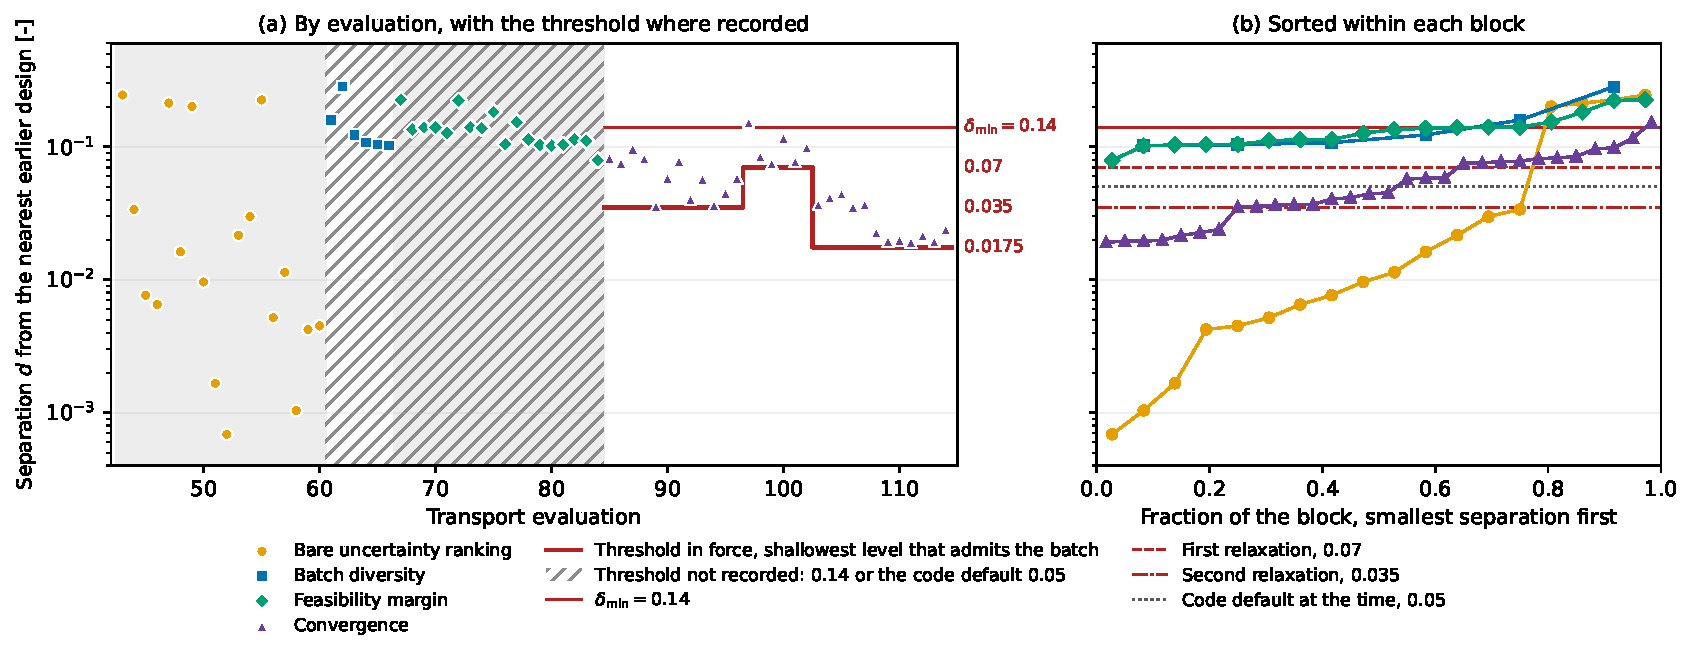
\includegraphics[width=0.95\linewidth]{images/c6_collapse}
  \caption{Campaign 6: separation of each infill design from the nearest earlier design. (a)~By evaluation. (b)~Sorted within each block.}
  \label{fig:c6-collapse}
\end{figure}

  \item \textbf{Unconstrained acquisition:} with the separation
        restored to 0.102, the second block returned one feasible design of 6, 5 exceeding the upper reactivity bound of 1.35 by
        1530 to \SI{7750}{pcm} while the constraint surrogate predicted all 6 feasible (Figure~\ref{fig:c6-margin}), and the
        feasibility margin of Equation~\eqref{eq:feas-margin} entered
        the third block.
\end{itemize}

\begin{figure}[htbp]
  \centering
  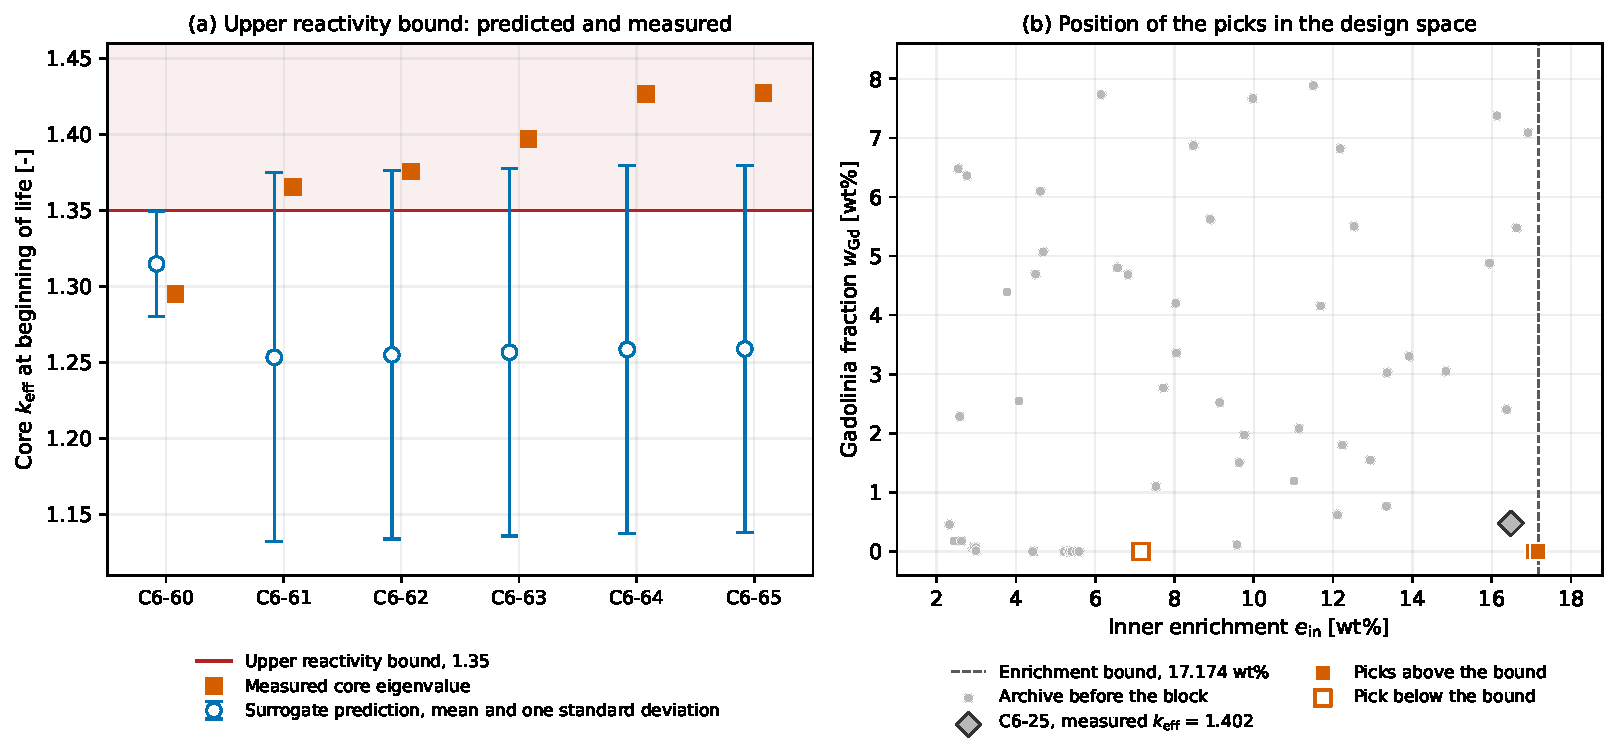
\includegraphics[width=0.85\linewidth]{images/c6_margin}
  \caption{Campaign 6, batch-diversity block: predicted and measured core multiplication factor and design-space position.}
  \label{fig:c6-margin}
\end{figure}

The effect of the feasibility margin is measured in two quantities:

\begin{itemize}
  \item \textbf{Hypervolume} (Figure~\ref{fig:c6-blocks}): no design of the
        2 blocks without the margin entered the Pareto front, so it stayed
        at its design-of-experiments value of 1287.99 over evaluations 43
        to 66. It increased by \SI{22.7}{\%} over the feasibility-margin
        block, to 1580.11, and the convergence block added \SI{1.4}{\%},
        to 1601.50.
  \item \textbf{Feasible fraction of the batches:} 0.72 and 0.17 in the 2
        blocks without the margin, 0.94 and 0.97 in the 2 with it.
\end{itemize}

Because
the hypervolume gain was zero in 2 blocks in which the search was not
converged, the stopping rule is necessary and not sufficient, which is
why the two health indicators of Section~\ref{sec:meth-loop-stop} are
computed at every iteration.

\begin{figure}[htbp]
  \centering
  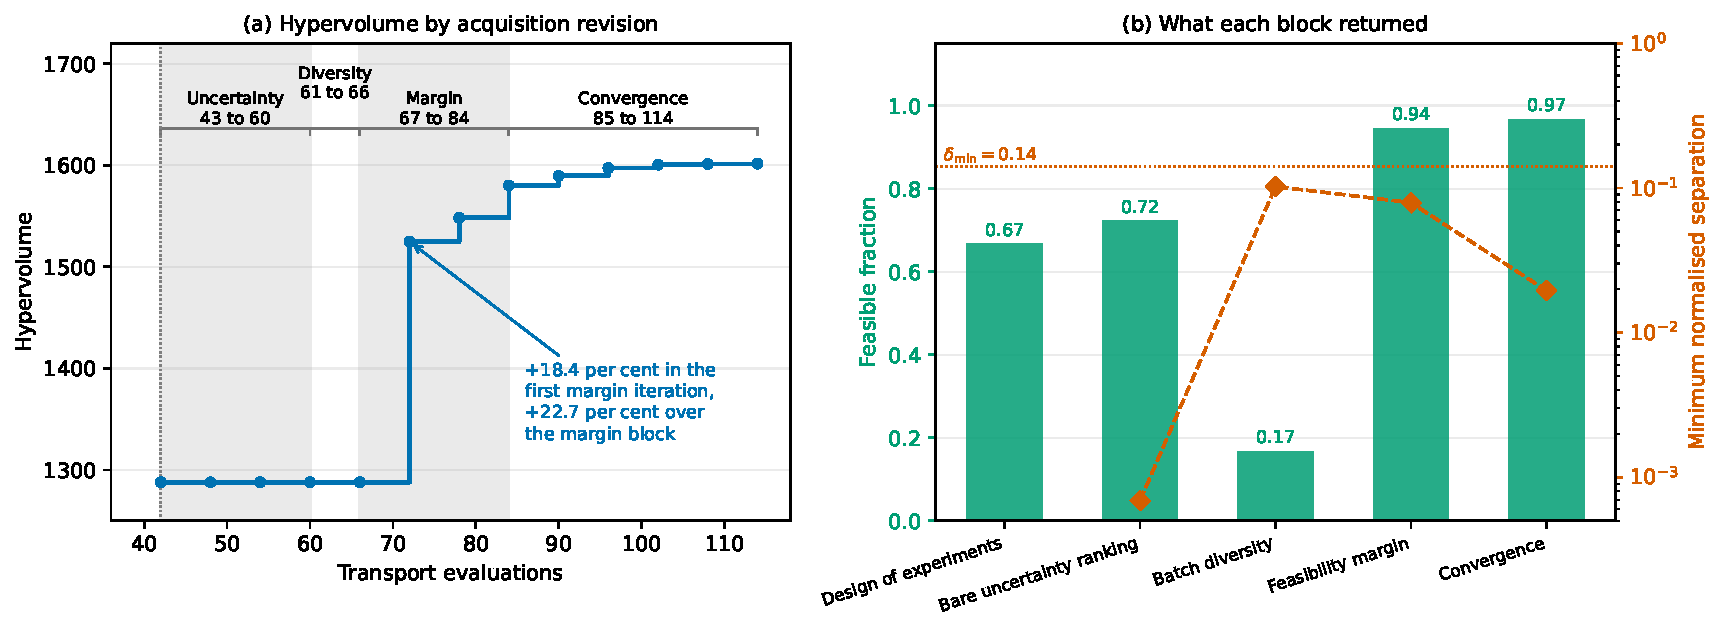
\includegraphics[width=\textwidth]{images/c6_blocks}
  \caption{Campaign 6: hypervolume by acquisition revision.}
  \label{fig:c6-blocks}
\end{figure}

\subsection{Search setting on the surrogate}
\label{sec:meth-nsga-setting}

From Campaign 6 the NSGA-II search on the surrogates uses a population
of 300 over 400 generations, in place of the $60\times80$ with which
Campaigns 1 to 5 started the loop. This setting was fixed by a
sensitivity study on fixed surrogates.
\label{sec:res-c6-search}
In that study the Gaussian processes were fitted once on the 42 designs
of the Campaign 6 design of experiments, and the search was repeated for
6 combinations of population size and number of generations, with 8
seeds each (Table~\ref{tab:nsga-sens}).

\begin{table}[htbp]
  \centering
  \caption{Campaign 6 design of experiments: sensitivity of the surrogate search.}
  \label{tab:nsga-sens}
  \begin{tabular}{lcccc}
    \toprule
    Setting & Hypervolume & Seed std & Distance & Time (s) \\
    \midrule
    $60\times80$   & 1903 & 12.72 & 0.000 & 0.45 \\
    $80\times120$  & 1913 & 20.41 & 0.073 & 0.82 \\
    $120\times160$ & 1932 &  5.95 & 0.097 & 1.47 \\
    $200\times200$ & 1940 &  1.67 & 0.088 & 2.82 \\
    $200\times400$ & 1943 &  1.36 & 0.095 & 5.63 \\
    $300\times400$ & 1945 &  0.59 & 0.102 & 8.22 \\
    \bottomrule
  \end{tabular}
\end{table}

Because the surrogates are the same in every search, any difference
between the seeds of one setting comes from the search alone, and the
criterion of the study is the seed-to-seed standard deviation of the
hypervolume of the surrogate front. If that standard deviation is
comparable to the differences between settings, two searches on the
same surrogate return different fronts, so the infill batch sent to
OpenMC depends on the random seed. If it is negligible, the search
returns the same front for every seed, so the batch is determined by
the surrogate. The adopted setting, $300\times400$, has a negligible
standard deviation in Table~\ref{tab:nsga-sens}, and its search takes
seconds against minutes for one transport evaluation, so the largest
setting tested adds no significant computing time.

\section{Core-level validation of the assembly proxy}
\label{sec:meth-core-objective}

Campaigns 1 to 3 minimised the radial peaking factor of the reflective
assembly (Section~\ref{sec:meth-fdh}). That value is a proxy of the core
value. It contains no radial power gradient between assemblies, so it
can rank designs differently from the core. Three instruments tested the
proxy against the core value, and their results are reported at the end
of this section. Campaign 4 then replaced the proxy with a direct core
calculation.

\begin{itemize}
  \item \textbf{Finalist validation:} each Pareto finalist is solved as
        the full core at the beginning of life with a pin-wise fission-power
        tally and replicated seeds. The ratio
        $F_{\Delta H}^\mathrm{core}/F_{\Delta H}^\mathrm{asm}$ is the
        model discrepancy, and the same solve checks the leakage-corrected $k_\mathrm{target}$ of Section~\ref{sec:meth-ktarget}.

  \item \textbf{Rescoring of the evaluated designs:} every feasible design is recomputed
        at core level, with 3 seeds and then eight near the minimum,
        and the Spearman rank correlation between proxy and core values
        measures whether the proxy discarded better designs.

  \item \textbf{Discrepancy model:} the multiplicative discrepancy
        between the 2 levels is fitted following Kennedy and
        O'Hagan~\cite{kennedy_ohagan_2000,forrester_book_2008}.
\end{itemize}

\begin{equation}
\frac{F_{\Delta H}^\mathrm{core}}{F_{\Delta H}^\mathrm{asm}}
\approx a + b\,t_\mathrm{refl} + c\,p
\label{eq:bridge}
\end{equation}

\noindent where the symbols have the following meaning.

\begin{itemize}
  \item $F_{\Delta H}^\mathrm{core}$ and $F_{\Delta H}^\mathrm{asm}$
        are the peaking factors of the same design at the core and assembly
        level, dimensionless.

  \item $a$ is the fitted intercept, dimensionless.

  \item $b$ is the fitted coefficient of the reflector thickness, in
        cm$^{-1}$.

  \item $c$ is the fitted coefficient of the pin pitch, in cm$^{-1}$.

  \item $t_\mathrm{refl}$ is the reflector thickness, in cm.

  \item $p$ is the pin pitch, in cm.
\end{itemize}

\label{sec:res-corevalidation}

Table~\ref{tab:core-finalists} gives the core solves of the finalists,
at $100\,000$ particles and up to 230 batches.

\begin{table}[htbp]
  \centering
  \begin{threeparttable}
  \caption{Campaign 3 finalists: core-level rescoring.}
  \label{tab:core-finalists}
  \small
  \setlength{\tabcolsep}{4pt}
  \begin{tabular}{lccccccc}
    \toprule
    & \multicolumn{3}{c}{Assembly} & \multicolumn{2}{c}{Core} & & \\
    \cmidrule(lr){2-4}\cmidrule(lr){5-6}
    & stored & corrected\tnote{a} & rank & $F_{\Delta H}$ (95\% CI)
      & rank & ratio & EFPD\tnote{b} \\
    \midrule
    C3-46 & 1.1397 & $1.1381$ & 6 & $2.013\pm0.018$ & 1 & 1.77 & 4\,307\tnote{c} \\
    C3-45 & 1.1522 & $1.1319$ & 5 & $2.020\pm0.019$ & 2 & 1.75 & 4\,307\tnote{c} \\
    C3-53 & 1.1445 & $1.1241$ & 3 & $2.114\pm0.018$ & 3 & 1.85 & 3\,396 \\
    C3-18 & 1.1270 & $1.1244$ & 4 & $2.126\pm0.018$ & 4 & 1.89 & 2\,082 \\
    C3-51 & 1.1266 & $1.1213$ & 2 & $2.153\pm0.015$ & 5 & 1.91 & 3\,108 \\
    C3-49 & 1.1336 & $1.1212$ & 1 & $2.159\pm0.032$ & 6 & 1.90 & 3\,189 \\
    \bottomrule
  \end{tabular}
  \begin{tablenotes}[flushleft]\footnotesize
    \item Ranks are among these 6 designs, lowest peaking first. The
      core solves use 8 seeds for the first 3 designs and 3 for the others.
    \item[a] Assembly value corrected for the bias of the search
      setting against $256\,000$ particles, on which the assembly rank
      is built.
    \item[b] Corrected for the restart defect of
      Section~\ref{sec:restart_defect}.
    \item[c] Right-censored at the depletion horizon, a lower bound.
  \end{tablenotes}
  \end{threeparttable}
\end{table}

The core solves establish three facts.

\begin{enumerate}
  \item \textbf{The model discrepancy is large and geometric:} The core
        value exceeds the assembly value by a factor of 1.75 to 1.91,
        anti-correlated with the reflector thickness at $r = -0.96$ over
        the 6 finalists. Thin reflectors leak, depress the periphery
        and raise the core-wide peaking, which an infinite lattice cannot
        see.

  \item \textbf{The ranking inverts:} Over the 6 finalists solved at
        core level the Spearman rank correlation between the
        bias-corrected assembly value and the core value is $-0.94$, and
        the assembly-best design, C3-49 at \num{1.1212}, is core-worst
        at \num{2.159}. The burnup-limited pair, C3-46 and C3-45, both at $|t| = 0.54$, beats the plateau at $|t| \approx 7$ to 8, so
        the front collapses to the burnup-limited strategy.

  \item \textbf{The peaking constraint becomes active:} Inactive
        everywhere at assembly level, it is violated by every design at
        core level, the best sitting at $2.013 \pm 0.018$ against the
        limit of 2.0.
\end{enumerate}

The 6 finalists are too few to establish the finding on their own,
so all 36 feasible designs of the campaign were rebuilt as uniform
cores and rescored (Figure~\ref{fig:asmcore}). Over all of them the
Spearman rank correlation between the assembly and the core value is
$+0.890$, yet 21 of the 36 move by 3 places or more between the
two models and the largest movements are of 10 places, C3-51 from
first on the assembly to eleventh on the core. The designs that move
are the ones near the front, where the optimiser spends its
evaluations, so a global correlation is no defence of a proxy, which is
the mechanism stated in Section~\ref{sec:bg-proxy}.

\begin{figure}[htbp]
  \centering
  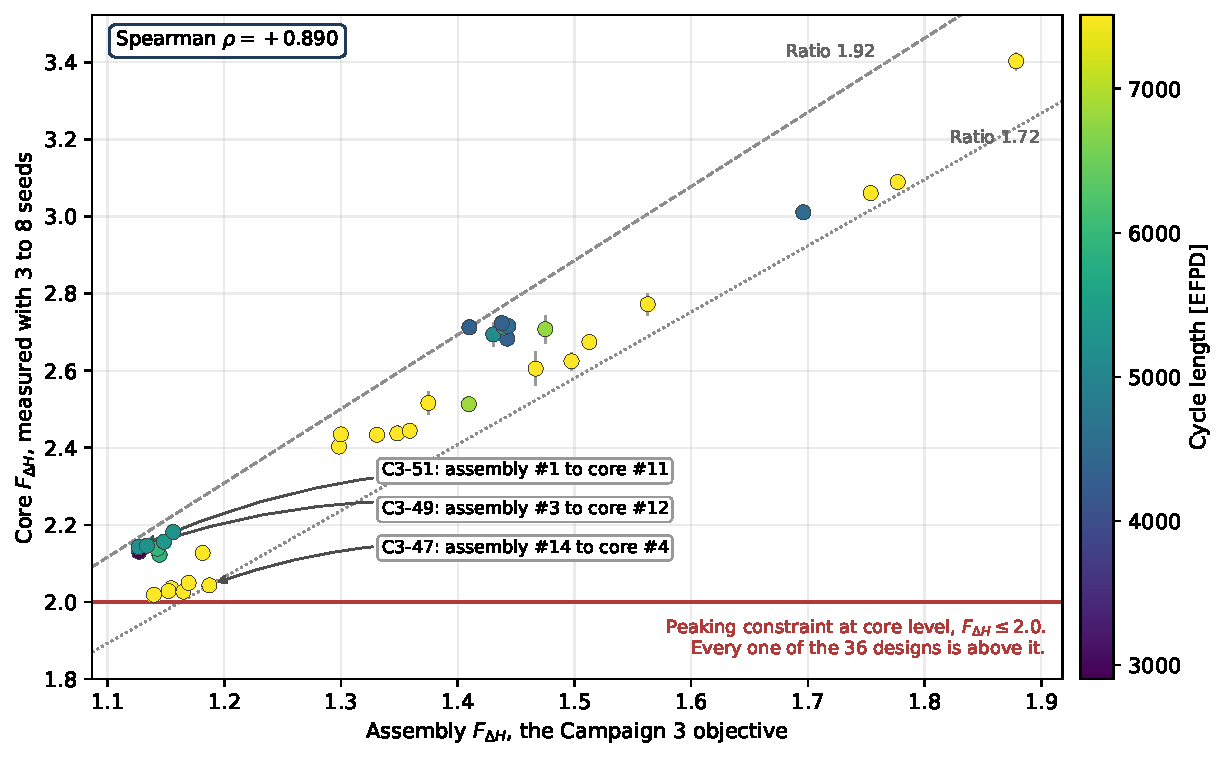
\includegraphics[width=0.78\linewidth]{images/th_asm_vs_core}
  \caption{Campaign 3 feasible designs: peaking factor rescored at core level.}
  \label{fig:asmcore}
\end{figure}

The bridge model of Equation~\eqref{eq:bridge}, fitted on all 36 designs,
\begin{equation}
  \frac{F^\mathrm{core}}{F^\mathrm{asm}}
  = 1.400 \;-\; 0.0045\,t_\mathrm{refl} \;+\; 0.343\,p,
  \qquad R^2 = 0.746,
  \label{eq:bridge-fit}
\end{equation}
confirms the reflector thickness and the pitch as the regressors that
govern the ratio. Its coefficient of determination of 0.746 leaves a
quarter of the variance unexplained, and that residual is the error of
any assembly value corrected with the fit. The core value is
therefore measured on each design rather than predicted, and the fit
holds for the uniform loading alone.

The same core solves compare the $k_\mathrm{target}$ the campaign
used with the core effective multiplication factor of each finalist,
with residuals of $-91$ to \SI{-429}{pcm}, most negative for the thick
reflectors.

These results and the cost of the change determined Campaign 4. The
core solve at beginning of life takes about \SI{104}{s} against an
evaluation of about \SI{110}{min}, and adding it increases the wall time
of one evaluation by about \SI{3}{\%}. From Campaign 4, $F_{\Delta H}$
and $g_\mathrm{peak}$ are therefore evaluated on the core solve of every
evaluation, and the assembly value is stored as a diagnostic quantity.
The cycle length is still obtained from the assembly depletion with the
leakage-corrected $k_\mathrm{target}$, because a full-core depletion in
every evaluation is not affordable, so the cycle-length proxy is kept.

\section{Validation of the optimisation framework}
\label{sec:validation-framework}

Two questions are answered before the fronts of Campaigns 8 and 9 are
interpreted, one in each of the next subsections.

\begin{enumerate}
  \item Whether the surrogate on which the acquisition was computed
        predicts the transport results accurately enough, with
        calibrated uncertainties
        (Section~\ref{sec:validation-surrogate}).

  \item Whether the front is a converged set rather than an artefact of
        the evaluation at which the campaign stopped or of the Monte
        Carlo noise of the transport solves
                (Section~\ref{sec:validation-front}).
\end{enumerate}

Both are answered on the database of every design evaluated by the
transport code with its objectives and constraints, for both
campaigns.

\subsection{Cross-validation of the surrogate on the evaluated designs}
\label{sec:validation-surrogate}

The surrogate under test is the surrogate of the loop
(Section~\ref{sec:meth-loop}), with the kernel of
Equation~\eqref{eq:kernel}, the standardisation of
Equation~\eqref{eq:standardise} and the normalised constraints of
Equation~\eqref{eq:cv-norm}, fitted on all evaluated designs, feasible
and infeasible.

Two validation schemes are applied (Figure~\ref{fig:val-protocols}).
The first is cross-validation of the surrogate against the data it was
fitted on, standard practice in engineering
design~\cite{forrester_book_2008}. The second applies the same idea to
the sequence of the loop, in which each infill batch was decided by the
surrogate fitted before that batch was evaluated.

\begin{itemize}
  \item \textbf{Leave-one-out cross-validation (LOOCV):} each of the $N$
        evaluated designs is held out once, and the surrogate refitted on
        the other $N-1$ designs predicts it. This is the leave-one-out
        predictive check of a Gaussian process~\cite{rasmussen_gp_2006},
        and it measures the predictive accuracy of the surrogate trained
        on all evaluated designs.

  \item \textbf{Walk-forward validation:} for each infill block, the
        surrogate trained only on the evaluations completed before that
        block predicts the designs of the block. It measures the
        predictive accuracy at the time of the acquisition decision, on
        the designs that the acquisition selected. In Campaign 9 the
        front predicted by the last refit was also evaluated by
        transport, which tests the prediction where the search would go
        next (Section~\ref{sec:res-c9-validation}).
\end{itemize}

\begin{figure}[htbp]
  \centering
  \resizebox{\textwidth}{!}{%
  \begin{tikzpicture}[
      box/.style={draw, rounded corners=2pt, align=center, font=\small,
                  text width=2.6cm, minimum height=1.25cm, fill=blue!6},
      lab/.style={font=\small\bfseries, align=right, text width=2.3cm},
      arr/.style={-{Stealth[length=2.2mm]}, thick},
      node distance=0.45cm]
    \node[lab] (l1) {Leave-one-out};
    \node[box, right=of l1] (a1) {$N$ evaluated designs};
    \node[box, right=of a1] (b1) {Remove design $i$};
    \node[box, right=of b1] (c1) {Refit the GPs on $N-1$ designs};
    \node[box, right=of c1] (d1) {Predict design $i$};
    \node[box, right=of d1] (e1) {Compare with the transport value};
    \draw[arr] (a1) -- (b1);
    \draw[arr] (b1) -- (c1);
    \draw[arr] (c1) -- (d1);
    \draw[arr] (d1) -- (e1);
    \draw[arr] (e1.south) -- ++(0,-0.35) -| node[pos=0.25, below, font=\footnotesize]
      {next $i$, until $i = N$} (b1.south);
    \node[lab, below=1.5cm of l1] (l2) {Walk-forward};
    \node[box, right=of l2] (a2) {Evaluations before block $b$};
    \node[box, right=of a2] (b2) {Fit the GPs};
    \node[box, right=of b2] (c2) {Predict the designs of block $b$};
    \node[box, right=of c2] (d2) {Compare with the transport values};
    \node[box, right=of d2] (e2) {Add block $b$ to the training set};
    \draw[arr] (a2) -- (b2);
    \draw[arr] (b2) -- (c2);
    \draw[arr] (c2) -- (d2);
    \draw[arr] (d2) -- (e2);
    \draw[arr] (e2.south) -- ++(0,-0.35) -| node[pos=0.25, below, font=\footnotesize]
      {next block $b+1$} (a2.south);
  \end{tikzpicture}}
  \caption{Surrogate validation: leave-one-out and walk-forward schemes.}
  \label{fig:val-protocols}
\end{figure}

For each output, the held-out predictions give the root mean square
error (RMSE) of the predictive mean against the transport value, the
coefficient of determination $R^2$, and the calibration of the
predictive uncertainty.

\begin{equation}
  s_z = \sqrt{\frac{1}{N}\sum_{i=1}^{N}\left(z_i - \bar{z}\right)^2},
  \qquad z_i = \frac{y_i - \mu_i}{\sigma_i}
  \label{eq:val-sz}
\end{equation}

\noindent where the symbols have the following meaning.

\begin{itemize}
  \item $y_i$ is the transport value of design $i$.
  \item $\mu_i$ and $\sigma_i$ are the predictive mean and standard
        deviation.
  \item $\bar{z}$ is the mean of the $N$ standardised residuals $z_i$,
        dimensionless.
  \item $s_z$ is their standard deviation, dimensionless, equal to 1 for
        a calibrated predictor, above 1 for an over-confident one and
        below 1 for an under-confident one.
\end{itemize}

Three further measures complete the set, the coverage of the one-sigma
and of the two-sigma predictive intervals, with nominal values 0.683 and
0.954 for Gaussian errors, and the Spearman rank correlation between
predicted and true values. The rank correlation is included because the
acquisition ranks the candidates and does not read their absolute
values. The constraint columns are converted back to the multiplication
factors they encode, so their errors are read in reactivity units.

In Campaign 9 the surrogate is also scored on its feasibility
classification, with two rules compared against the feasibility of the
transport solves. The mean rule declares a design feasible when every
predicted constraint mean is at or below zero. The margin rule, which
the acquisition uses, declares it feasible when every predicted
constraint mean plus $\kappa$ predictive standard deviations is at or
below zero, with $\kappa$ the campaign value of
Section~\ref{sec:meth-acq}.

The results are reported in Section~\ref{sec:res-c8-cv} for Campaign 8
and in Section~\ref{sec:res-c9-validation} for Campaign 9.

\subsection{Stability of the campaign front}
\label{sec:validation-front}

The front is the result the campaign delivers, so it must be shown to
be converged and not an artefact of the evaluation at which the
campaign stopped or of the Monte Carlo noise of the transport solves.
One test addresses each of these two possibilities.

\begin{enumerate}
  \item \textbf{Membership through the campaign:} the first test
        tracks the front as the campaign builds it, with the
        hypervolume of the non-dominated set as its convergence
        measure~\cite{coello_2007}. The feasible non-dominated set is
        recomputed after every evaluation, in the order of execution,
        together with its hypervolume at the fixed reference point,
        defined once from the design of experiments of the campaign.
        For each member of the final front, the evaluation at which it
        joined the set is stored. A front whose
        members all joined in the first blocks and were never removed
        is converged. A front that gains a member in its last block is
        not, and its membership depends on where the campaign stopped.

        This is a different question from the stopping rule of
        Section~\ref{sec:meth-loop-stop}. That rule is a decision taken
        during the campaign on one scalar, the relative gain of the
        hypervolume, and it fires when that gain stays below one per
        cent for 3 iterations. A design can join the front at the
        last evaluation while contributing almost nothing to the
        hypervolume, so the rule can be satisfied on a front whose membership
        is still changing. The test reads the membership itself, after
        the campaign.

  \item \textbf{Membership under the transport noise:} the second test
        perturbs the front, which is the treatment of an objective
        carrying a Monte Carlo uncertainty applied to an optimisation
        based on such solves~\cite{erdem_2025_mc_uncertainty}. Each
        objective of every feasible design is perturbed by Gaussian
        noise of its own Monte Carlo standard deviation, the non-dominated set is recomputed, and the
        probability that each design belongs to it is estimated over
        many replicates. Where the cycle length is an objective, its noise results
        from the uncertainty of the multiplication factor through the mean reactivity
        slope of the design.

        \begin{equation}
          \sigma_{\mathrm{cycle}} = \sqrt{2}\,\frac{\sigma_k}{\left(k_{\infty,\mathrm{BOL}} - k_{\mathrm{target}}\right)/T}
          \label{eq:val-sigma-cycle}
        \end{equation}

        \noindent where the symbols have the following meaning.

        \begin{itemize}
          \item $\sigma_\mathrm{cycle}$ is the one-sigma noise on the
                cycle length, in EFPD.
          \item $\sigma_k$ is the one-sigma uncertainty of the infinite
                multiplication factor at one depletion step,
                dimensionless.
          \item $k_{\infty,\mathrm{BOL}}$ is the beginning-of-life
                multiplication factor of the assembly, dimensionless.
          \item $k_\mathrm{target}$ is the leakage-corrected end-of-cycle
                multiplication factor of Section~\ref{sec:meth-ktarget},
                dimensionless.
          \item $T$ is the campaign cycle length, in EFPD.
          \item $\sqrt{2}$ accounts for the interpolation of the
                end-of-cycle crossing between two independently noisy
                multiplication factors.
        \end{itemize}
\end{enumerate}

Two front members whose membership probabilities are well below one are
not statistically distinguishable under the transport noise and are
reported as
equivalent. The results of both tests are reported in
Section~\ref{sec:res-c8-stability} for Campaign 8 and in
Sections~\ref{sec:res-c9-convergence} and~\ref{sec:res-c9-validation}
for Campaign 9.

\section{Source convergence, computing environment and reproducibility}
\label{sec:meth-diagnostics}

Every campaign is documented in three respects:

\begin{itemize}
  \item \textbf{Source convergence:} the Shannon entropy of the fission
        source is monitored in every model and the batch at which each
        calculation becomes stationary is stored by the evaluator, as
        Figure~\ref{fig:entropy} illustrates. Over the 309 assembly and
        238 core solves of the stored campaigns, the reflective
        assembly is stationary from the first batch, while the finite
        core has a transient with a median of 12.5 batches and a maximum
        of 114. This transient is why the core solves use 60 inactive
        batches from Campaign 4 onward. In 27 of the 238 core solves the
        source became stationary only after those 60 batches, 5 of them
        in Campaign 8 and 2 in Campaign 9, none on the front of its
        campaign. Such a solve biases its own beginning-of-life peaking
        factor, but not the ordering used by the design of experiments
        and the infill selection, so the campaigns were completed
        without being executed again. A further campaign should raise
        the number of inactive batches above 60.

        \begin{figure}[htbp]
          \centering
          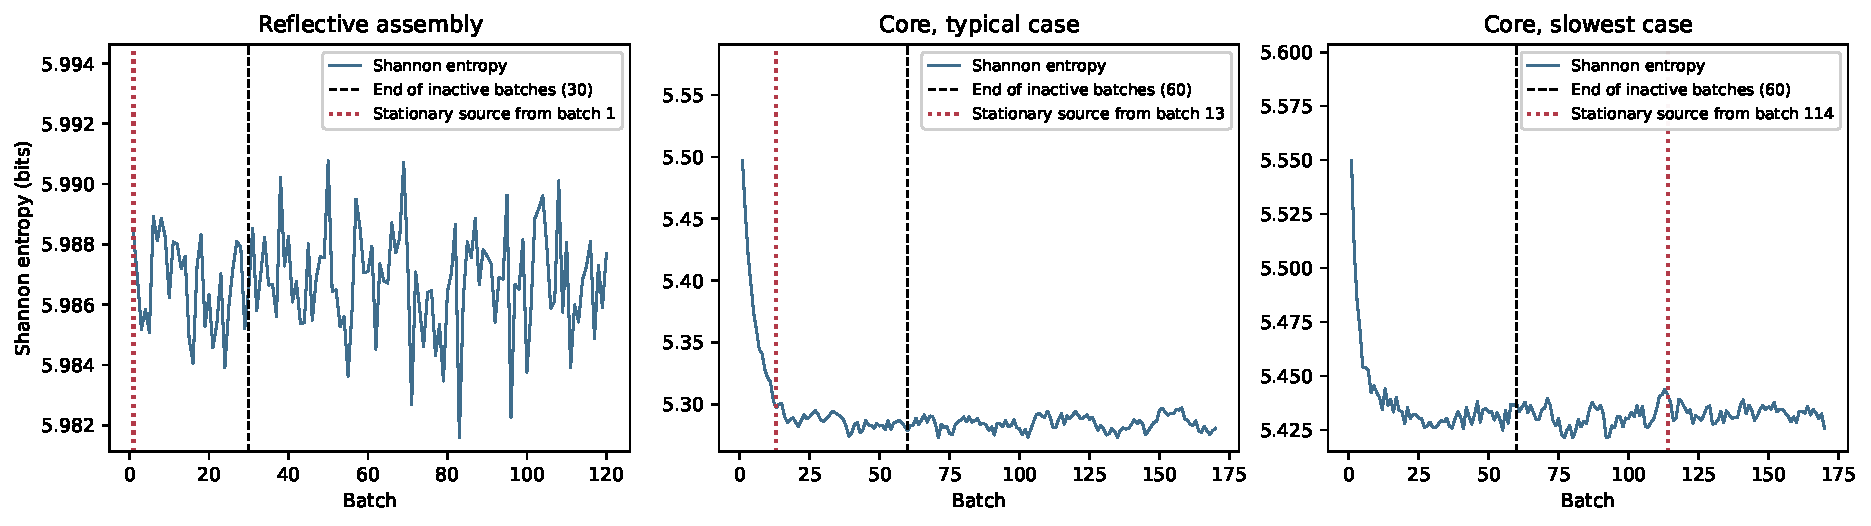
\includegraphics[width=\textwidth]{images/th_entropy.pdf}
          \caption{Source convergence: Shannon entropy per batch of the reflective assembly, a typical core solve and the slowest core solve.}
          \label{fig:entropy}
        \end{figure}

  \item \textbf{Computing environment:} Table~\ref{tab:host-specs}
        gives the processor, memory, operating system and campaigns of
        each host. Both hosts use the same Conda environment, defined in
        the repository, with Python 3.13.13, OpenMC 0.15.3,
        pymoo 0.6.2 and scikit-learn 1.9.0.

\begin{table}[htbp]
  \centering
  \small
  \caption{Computing hosts: configuration and campaigns.}
  \label{tab:host-specs}\label{tab:hosts}
  \begin{tabularx}{\textwidth}{@{}l>{\raggedright\arraybackslash}X>{\raggedright\arraybackslash}X@{}}
    \toprule
    Characteristic & Cloud instance & Workstation \\
    \midrule
    Machine & AWS EC2 c7a.8xlarge, on demand & wks720 \\
    Processor & AMD EPYC 9R14, fourth generation (Genoa) & AMD Ryzen Threadripper 2990WX (Zen+, 12\,nm) \\
    Physical cores & 32 & 32 \\
    Logical processors & 32, simultaneous multithreading disabled & 64, two per core \\
    Clock frequency & Up to \SI{3.7}{GHz} & \SI{3.0}{GHz} base, \SI{4.2}{GHz} boost \\
    Memory & \SI{64}{GiB} & \SI{62}{GiB} available to the operating system \\
    Operating system & Ubuntu Server 24.04, Docker container & Linux Mint 22, kernel 6.8 \\
    Environment & Docker image with the pinned Conda environment & Pinned Conda environment, no administrative privileges \\
    Campaigns & 1, 2, 6 and 7 & 3 to 5, 8 and 9 \\
    \bottomrule
  \end{tabularx}
\end{table}

  \item \textbf{Sources of randomness:} three enter a campaign, and they
        differ in whether they are seeded.

        \begin{enumerate}
          \item Each transport solve is seeded from its own design
                vector (Section~\ref{sec:meth-fidelity}), so every evaluated design reproduces its beginning-of-life solves exactly and its depletion within its statistical error.

          \item The Gaussian-process hyperparameter optimisation and
                the NSGA-II search on the surrogate are seeded.

          \item The Latin-hypercube design of experiments is not
                seeded. The sampling routine of the framework declares a
                seed argument but never forwards it to the pymoo
                Latin-hypercube operator, which is therefore constructed
                without one and samples from the global state of the
                NumPy generator. Three launches with the same configured
                seed returned three different initial design matrices.
                The same routine generates the space-filling designs
                that complete a batch when the sequential selection
                under the minimum-distance constraint
                $\delta_\mathrm{min}$ of the batch-diversity revision
                of Section~\ref{sec:meth-acq} leaves no admissible candidate,
                so those points are not reproducible either.
        \end{enumerate}

        A campaign relaunched from scratch therefore starts from a
        different design of experiments and takes a different
        trajectory. Each campaign is documented by its stored checkpoint, which stores every evaluated design with its inputs,
        outputs and the fixed hypervolume reference point, and every
        result of Chapter~\ref{ch:results} is computed from it. The
        checkpoints are stored in the public code repository of this
        thesis, described in
        Appendix~\ref{app:code-architecture}. The
        surrogate-search study of Section~\ref{sec:meth-nsga-setting} is
        not affected, because it starts from fixed training data and uses
        only the seeded search.
\end{itemize}

